% dissertaion.tex
%
% Based on the example from Paul Vojta.

\documentclass{ucbthesis}
\usepackage{biblatex}

% If the Grad. Division insists that the first paragraph of a section
% be indented (like the others), then include this line:
% \usepackage{indentfirst}

\newtheorem{theorem}{Jibberish}

\bibliography{dissertation}
\usepackage{xspace}
\usepackage{url}
\usepackage{latexsym}
\usepackage{multirow}
\usepackage{graphicx}
\usepackage{amsmath}
\usepackage{subfig}
\usepackage{color}
\usepackage{pstricks}
\usepackage{algorithm}
\usepackage{algpseudocode}
\usepackage{synttree}

% TODO - switch away from syntax tree entirely
% Syntax-tree settings
\branchheight{0.33in}
\trianglebalance{50}
\childsidesep{1em}
\childattachsep{0.5in}
\newcommand{\derivscale}{0.7}
\newcommand{\derivspace}{\vspace{-4mm}}
\newcommand{\derivaftercompress}{\vspace{-2mm}}

\setcounter{totalnumber}{500}
\setcounter{topnumber}{500}
\setcounter{bottomnumber}{500}

\newcommand{\nlp}{\textsc{nlp}\xspace}
\newcommand{\wsj}{\textsc{wsj}\xspace}
\newcommand{\ptb}{\textsc{ptb}\xspace}
\newcommand{\parseval}{\textsc{parseval}\xspace}
\newcommand{\evalb}{\textsc{evalb}\xspace}
\newcommand{\cky}{\textsc{cky}\xspace}
\newcommand{\pos}{\textsc{pos}\xspace}
\newcommand{\dop}{\textsc{dop}\xspace}

\newcommand{\schwa}{\acronym{schwa}}
\newcommand{\schwalab}{\raisebox{.45em}{\rotatebox{180}{e}}-lab}

\newcommand{\eg}{e.g.\@\xspace}
\newcommand{\ie}{i.e.\@\xspace}

\newcommand{\smallsf}{\small\sf}
 
\newcommand{\wrongnode}[1]{\textbf{\fbox{#1}}}

% Example of specifying allowed hyphenation within a word
% \hyphenation{mar-gin-al-ia}

\begin{document}

% Declarations for Front Matter

\title{Eulerian Knowledge Prexy and Lyman Zig on Wiggly}
\author{Jonathan K. Kummerfeld}
\degreesemester{Summer}
\degreeyear{2016}
\degree{Doctor of Philosophy}
\chair{Professor Dan Klein}
\othermembers{Professor Marti A. Hearst \\
  Associate Professor Line Mikkelsen}
\numberofmembers{3}
\field{Computer Science}
\campus{Berkeley}

\maketitle
% TODO: Delete (or comment out) the \approvalpage line for the final version.
\approvalpage
\copyrightpage

\begin{abstract}

Representation of syntactic structure is a core area of research in Computational Linguistics, disambiguating distinctions in meaning that are crucial for correct interpretation of language.
Development of algorithms and statistical models over the past three decades has led to systems that are accurate enough to be deployed in industry, playing a key role in products such as Google Search and Apple Siri.
However, syntactic parsers today are usually constrained to tree representations of language, and performance is interpreted through a single metric that conveys no linguistic information regarding remaining errors.

In this dissertation, we present new algorithms for error analysis and parsing.
The heart of our approach to error analysis is the use of structural transformations to identify more meaningful classes of errors, and to enable comparisons across formalisms.
For parsing, we combine a novel dynamic program with careful choices in syntactic representation to create an efficient parser that produces graph structured output.
In both cases, we are pushing the boundaries of the conventional parsing task, bringing it closer to the linguistic theories it is based on.

First, we present a search algorithm that, given two structures, finds a sequence of modifications leading from one structure to the other.
We applied this algorithm to syntactic error analysis, where one structure is the output of a parser, the other is the correct parse, and each modification corresponds to fixing one error.
We constructed a tool based on the algorithm and analyzed variations in behavior between parsers, types of text, and languages.
Our observations shine light on several assumptions about syntactic errors, showing some to be true and others to be false.
For example, prepositional phrase attachment errors are indeed a major issue, while coordination scope errors do not hurt performance as much as expected.

Next, we describe an algorithm that builds a parse in one syntactic representation based on a parse in another.
Specifically, we build phrase structure parses from Combinatory Categorial Grammar derivations.
Our approach follows the philosophy of \ccg, defining specific phrase structures for each lexical category and generic rules for combinatory steps.
The new parse is built by following the \ccg derivation bottom-up, gradually building the corresponding phrase structure parse.
This produces significantly more accurate parses than past work, and has the advantage that the process decomposes in the same way as the CKY parsing algorithm.
We use the tool to compare performance of parsers across formalisms % TODO

Finally, we present a dynamic programming algorithm, which constructs the graph structure that has the highest score under an edge-factored scoring function.
In the process of defining a parse representation compatible with the algorithm, we found that certain linguistic distinctions could dramatically impact coverage.
We also show various ways to modify the algorithm to improve performance by exploiting properties of observed linguistic structure.
This approach to syntactic parsing is the first to cover virtually all structure encoded in the Penn Treebank.


\end{abstract}


\begin{frontmatter}

%%%\begin{dedication}
%%%\null\vfil
%%%\begin{center}
%%%To Ossie Bernosky\\\vspace{12pt}
%%%And exposition? Of go. No upstairs do fingering. Or obstructive, or purposeful.
%%%In the glitter. For so talented. Which is confines cocoa accomplished.
%%%Masterpiece as devoted. My primal the narcotic. For cine? To by recollection
%%%bleeding. That calf are infant. In clause. Be a popularly. A as midnight
%%%transcript alike. Washable an acre. To canned, silence in foreign.
%%%\end{center}
%%%\vfil\null
%%%\end{dedication}

\tableofcontents
\clearpage
\listoffigures
\clearpage
\listoftables

\begin{acknowledgements}
Acknowledgements!
\end{acknowledgements}

\end{frontmatter}

\pagestyle{headings}

\include{intro}
\chapter{Automatic Error Analysis}

%%% TODO:
%%% - Add 'treebank', 'parser' sideways labels to figures
%%%	Something else to think about - this paper is about 'what',
%%%	not 'why', so we don't use concepts like subcategorisation
%%%	Errors related to temporal structures would be a sensible
%%%	part though

Previously published as "Parser Showdown at the Wall Street Corral: An Empirical Investigation of Error Types in Parser Output", Jonathan K. Kummerfeld, David Hall, James R. Curran and Dan Klein.

\section{Parsers}

Our evaluation is over a wide range of \ptb constituency parsers and their variants from the past fifteen years.
For all parsers we used the publicly available version, with the standard parameter settings.

\begin{description}\itemsep1pt
	\item[ Berkeley] \cite{Petrov-etal:2006,Petrov-Klein:2007}. An
	unlexicalised parser with a grammar constructed with automatic state
	splitting.

	\item[ Bikel] (2004)\nocite{Bikel:2004} implementation of Collins (1997).

	\item[ BUBS]
	\cite{Dunlop-Bodenstab-Roark:2011,Bodenstab-Dunlop-Hall-Roark:2011}. A
	`grammar-agnostic constituent parser,' which uses a Berkeley Parser grammar,
	but parses with various pruning techniques to improve speed, at the cost of
	accuracy.

	\item[ Charniak] (2000)\nocite{Charniak:2000}. A generative parser with a
	maximum entropy-inspired model.  We also use the reranker
	\cite{Charniak-Johnson:2005}, and the self-trained model
	\cite{McClosky-Charniak-Johnson:2006}.

	\item[ Collins] (1997)\nocite{Collins:1997}. A generative lexicalised parser, with
	three models, a base model, a model that uses subcategorisation
	frames for head words, and a model that takes into account traces.

	\item[ SSN] \cite{Henderson:2003,Henderson:2004}. A statistical left-corner
	parser, with probabilities estimated by a neural network.

	\item[ Stanford] \cite{Klein-Manning:2003,Klein-Manning:2003:NIPS}. We
	consider both the unlexicalised PCFG parser (-U) and the factored parser
	(-F), which combines the PCFG parser with a lexicalised dependency parser.
\end{description}

\begin{table}
%%%\small
%%%\renewcommand{\tabcolsep}{1.7mm}
\begin{center}
\begin{tabular}{|lccccr|}
	\hline
		System & F & P & R & Exact & Speed \\
	\hline
	\hline
		\multicolumn{6}{|c|}{enhanced training / systems} \\
		Charniak-SR & 92.07 & 92.44 & 91.70 & 44.87 & 1.8 \\
		Charniak-R & 91.41 & 91.78 & 91.04 & 44.04 & 1.8 \\
		Charniak-S & 91.02 & 91.16 & 90.89 & 40.77 & 1.8 \\
	\hline
		\multicolumn{6}{|c|}{standard parsers} \\
		Berkeley & 90.06 & 90.30 & 89.81 & 36.59 & 4.2 \\
		Charniak & 89.71 & 89.88 & 89.55 & 37.25 & 1.8 \\
		SSN & 89.42 & 89.96 & 88.89 & 32.74 & 1.8 \\
		BUBS & 88.50 & 88.57 & 88.43 & 31.62 & 27.6 \\
		Bikel & 88.16 & 88.23 & 88.10 & 32.33 & 0.8 \\
		Collins-3 & 87.66 & 87.82 & 87.50 & 32.22 & 2.0 \\
		Collins-2 & 87.62 & 87.77 & 87.48 & 32.51 & 2.2 \\
		Collins-1 & 87.09 & 87.29 & 86.90 & 30.35 & 3.3 \\
		Stanford-L & 86.42 & 86.35 & 86.49 & 27.65 & 0.7 \\
		Stanford-U & 85.78 & 86.48 & 85.09 & 28.35 & 2.7 \\
	\hline
\end{tabular}
\caption{
	\label{tab:standard-results} \parseval results on \wsj section 23 for
	the parsers we consider.  The columns are F-score, precision, recall,
	exact sentence match, and speed (sents/sec).  Coverage was left out
	as it was above 99.8\% for all parsers.  In the {enhanced training /
	systems} section we include the Charniak parser with reranking (R), with a
	self-trained model (S), and both (SR).
}
\end{center}
%%%\vspace{-3mm}
\end{table}

Table~\ref{tab:standard-results} shows the standard performance metrics,
measured on section 23 of the \wsj, using all sentences.  Speeds were measured
using a Quad-Core Xeon CPU (2.33GHz 4MB L2 cache) with 16GB of RAM.
These results clearly show the variation in parsing performance, but they do
not show which constructions are the source of those variations.

\begin{figure}
\begin{center}
\scalebox{\derivscale}{
\synttree
[S
	[NP
		[PRP [He]]]
	[VP
		[VBD [was]]
		[VP
			[VBN [named]]
			[\wrongnode{S}
				[\wrongnode{NP}
					[NP [.t chief executive officer]]
					[\wrongnode{PP}
						[IN [of]]
						[\wrongnode{NP}
							[NP
								[NNP [Applied]]]
							[PP [.t in 1986]]]]]]]]]
}

\small
(a) Parser output
\vspace{3mm}

\scalebox{\derivscale}{
\synttree
[S
	[NP
		[PRP [He]]]
	[VP
		[VBD [was]]
		[VP
			[VBN [named]]
			[\wrongnode{S}
				[\wrongnode{NP}
					[NP [.t chief executive officer]]
					[\wrongnode{PP}
						[IN [of]]
						[NP
							[NNP [Applied]]]]]]
			[PP [.t in 1986]]]]]
}

\small
(b) Gold tree
\end{center}
\derivspace
\caption{
	\label{fig:PP-attachment}
	Grouping errors by node type is of limited usefulness.  In this figure and
	those that follow the top tree is the incorrect parse and the bottom tree is
	the correct parse.  Bold, boxed nodes are either extra (marked in the
	incorrect tree) or missing (marked in the correct tree).  This is an example
	of \textbf{PP~Attachment} (\emph{in~1986} is too low), but that is not at all
	clear from the set of incorrect nodes (extra S, NP, PP, and NP, missing S,
	NP, and PP).
}
\derivaftercompress
\end{figure}

\section{Error Classification}

While the statistics in Table~\ref{tab:standard-results} give a sense of
overall parser performance they do not provide linguistically meaningful
intuition for the source of remaining errors.  Breaking down the remaining
errors by node type is not particularly informative, as a single attachment
error can cause multiple node errors, many of which are for unrelated node
types.  For example, in Figure~\ref{fig:PP-attachment} there is a PP attachment
error that causes seven bracket errors (extra S, NP, PP, and NP, missing S,
NP, and PP).  Determining that these correspond to a PP attachment error from
just the labels of the missing and extra nodes is difficult.  In contrast, the
approach we describe below takes into consideration the relations between
errors, grouping them into linguistically meaningful sets.

We classify node errors in two phases.  First, we find a set of tree
transformations that convert the output tree into the gold tree.  Second, the
transformation are classified into error types such as PP attachment and
coordination.  Pseudocode for our method is shown in Algorithm~\ref{alg:code}.
The tree transformation stage corresponds to the main loop, while the second
stage corresponds to the final loop.

\begin{algorithm}[t]
\small
\begin{algorithmic}
\small
\State $U =$ initial set of node errors
\State Sort $U$ by the depth of the error in the tree, deepest first
\State $G = \emptyset$
\Repeat
	\ForAll{errors $e \in U$}
		\If{$e$ fits an environment template $t$}
			\State $g =$ new error group
			\State Correct $e$ as specified by $t$
			\ForAll{errors $f$ that $t$ corrects}
				\State Remove $f$ from $U$
				\State Insert $f$ into $g$
			\EndFor
			\State Add $g$ to $G$
		\EndIf
	\EndFor
\Until{unable to correct any further errors}
\ForAll{remaining errors $e \in U$}
	\State Insert a group into $G$ containing $e$
\EndFor
\ForAll{groups $g \in G$}
	\State Classify $g$ based on properties of the group
\EndFor
\end{algorithmic}
\caption{\small
\label{alg:code}
	Tree transformation error classification
}
\end{algorithm}

\subsection{Tree Transformation}

The core of our transformation process is a set of operations that move
subtrees, create nodes, and delete nodes.  Searching for the shortest path to
transform one tree into another is prohibitively slow.\footnote{We implemented
various search procedures and found similar results on the sentences that could
be processed in a reasonable amount of time.}  We find a path by applying a
greedy bottom--up approach, iterating through the errors in order of tree depth.
%%%in the tree, deepest first.

We match each error with a template based on nearby tree structure and
errors.  For example, in Figure~\ref{fig:PP-attachment} there are four extra
nodes that all cover spans ending at \emph{Applied in 1986}: S, NP, PP, NP.
There are also three missing nodes with spans ending between \emph{Applied} and
\emph{in}: PP, NP, and S.  Figure~\ref{fig:template} depicts these errors as
spans, showing that this case fits three criteria: (1) there are a set of extra
spans all ending at the same point, (2) there are a set of missing spans all
ending at the same point, and (3) the extra spans cross the missing spans,
extending beyond their end-point.  This indicates that the node starting after
\emph{Applied} is attaching too low and should be moved up, outside all of the
extra nodes.  Together, the criteria and transformation form a template.

\begin{figure}
\begin{center}
%%%\begin{pspicture}(-0.07,-0.6)(7.9,0.6)
%%%\psline(1.02,0.16)(1.02,0.75)(7.85,0.75)(7.85,0.16)
%%%\psline(4.52,0.16)(4.52,0.65)(7.75,0.65)(7.75,0.16)
%%%\psline(5.03,0.16)(5.03,0.55)(7.65,0.55)(7.65,0.16)
%%%\psline[linestyle=dashed,dash=4pt 2pt](1.02,0.02)(1.02,-0.51)(6.35,-0.51)(6.35,0.02)
%%%\psline[linestyle=dashed,dash=4pt 2pt](4.52,0.02)(4.52,-0.41)(6.25,-0.41)(6.25,0.02)
%%%\small named$\;$ chief$\;$ executive$\;$ officer$\;$ of$\;$ Applied$\;$ in$\;$ 1986
%%%\end{pspicture}
\end{center}
\vspace{-5mm}
\caption{
	\label{fig:template}
	Templates are defined in terms of extra and missing spans, shown here with
	unbroken lines above and dashed lines below, respectively.  This is an
	example of a set of extra spans that cross a set of missing spans (which in
	both cases all end at the same position).  If the last two words are moved,
	two of the extra spans will match the two missing spans.  The other extra
	span is deleted during the move as it creates an NP$\rightarrow$NP unary
	production.
}
\vspace{-3.5mm}
\end{figure}

Once a suitable template is identified we correct the error by moving subtrees,
adding nodes and removing nodes.  In the example this is done by moving the
node spanning \emph{in 1986} up in the tree until it is outside of all the
extra spans.  Since moving the PP leaves a unary production from an NP to an
NP, we also collapse that level.  In total this corrects seven errors, as there
are three cases in which an extra node is present that matches a missing node
once the PP is moved.  All of these errors are placed in a single group and
information about the nearby tree structure before and after the transformation
is recorded.

We continue to make passes through the list until no errors are corrected on a
pass.  For each remaining node error an individual error group is created.

The templates were constructed by hand based on manual analysis of parser
output.  They cover a range of combinations of extra and missing spans, with
further variation for whether crossing is occurring and if so whether the
crossing bracket starts or ends in the middle of the correct bracket.
Errors that do not match any of our templates are left uncorrected.

\subsection{Transformation Classification}

We began with a large set of node errors, in the first stage they were placed
into groups, one group per tree transformation used to get from the test tree
to the gold tree.  Next we classify each group as one of the error types below.

\begin{description}\itemsep1pt
	\item[ PP Attachment] Any case in which the transformation involved moving
	a Prepositional Phrase, or the incorrect bracket is over a PP, \eg \\ 
	\emph{He was} (VP \emph{named chief executive officer of} \\
	\textcolor{white}{fill}(NP \emph{Applied} (PP \emph{in 1986}))) \\
	where (PP \emph{in 1986}) should modify the entire VP, rather than just \emph{Applied}.

	\item[ NP Attachment] Several cases in which NPs had to be moved,
	particularly for mistakes in appositive constructions and incorrect
	attachments within a verb phrase, \eg \\ \emph{The bonds} (VP \emph{go} (PP
	\emph{on} \emph{sale} (NP \emph{Oct.\@\xspace 19}))) \\
	where \emph{Oct.\@\xspace 19} should be an argument of \emph{go}.
\end{description}


\begin{figure}
\begin{center}
\scalebox{\derivscale}{
\synttree
[VP
	[VBD [wrote]]
		[\wrongnode{NP}
			[NP
				[DT [another]]
				[JJ [new]]
				[NN [ad]]]
			[VBG [appearing]]]
		[NP
			[NN [today]]]]
}

\small
(a) Parser output

\vspace{3mm}

\scalebox{\derivscale}{
\synttree
[VP
	[VBD [wrote]]
		[\wrongnode{NP}
			[NP
				[DT [another]]
				[JJ [new]]
				[NN [ad]]]
			[\wrongnode{VP}
				[VBG [appearing]]
				[NP
					[NN [today]]]]]]
}

\small
(b) Gold tree
\end{center}
\derivspace
\caption{
	\label{fig:NP-attachment}
	\textbf{NP Attachment}: \emph{today} is too high, it should be the argument
	of \emph{appearing}, rather than \emph{wrote}.  This causes three node errors
	(extra NP, missing NP and VP).
}
\derivaftercompress
\end{figure}

\begin{figure}
\begin{center}
\scalebox{\derivscale}{
\synttree
[VP
	[VBD [had]]
	[\wrongnode{S}
		[\wrongnode{VP}
			[TO [to]]
			[\wrongnode{VP}
				[VB [think]]
				[PP [.t about it]]]]]
	[ADVP [.t ahead of time]]]
}

\small
(a) Parser output

\vspace{3mm}

\scalebox{\derivscale}{
\synttree
[VP
	[VBD [had]]
	[\wrongnode{S}
		[\wrongnode{VP}
			[TO [to]]
			[\wrongnode{VP}
				[VB [think]]
				[PP [.t about it]]
				[ADVP [.t ahead of time]]]]]]
}

\small
(b) Gold tree
\end{center}
\derivspace
\caption{
	\label{fig:modifier-attachment}
	\textbf{Modifier Attachment}: \emph{ahead of time} is too high, it should
	modify \emph{think}, not \emph{had}.  This causes six node errors (extra
	S, VP, and VP, missing S, VP, and VP).
}
\derivaftercompress
\end{figure}

\begin{figure}
\begin{center}
\scalebox{\derivscale}{
\synttree
[VP
	[VBZ [intends]]
	[\wrongnode{S}
		[\wrongnode{VP}
			[TO [to]]
			[\wrongnode{VP}
				[VB [restrict]]
				[NP [.t the RTC to \ldots]]
				[SBAR [.t unless the agency \ldots]]]]]]
}

\small
(a) Parser output

\vspace{3mm}

\scalebox{\derivscale}{
\synttree
[VP
	[VBZ [intends]]
	[\wrongnode{S}
		[\wrongnode{VP}
			[TO [to]]
			[\wrongnode{VP}
				[VB [restrict]]
				[NP [.t the RTC to \ldots]]]]]
	[SBAR [.t unless the agency \ldots]]]
}

\small
(b) Gold tree
\end{center}
\derivspace
\caption{
	\label{fig:clause-attachment}
	\textbf{Clause Attachment}: \emph{unless the agency receives specific
	congressional authorization} is attaching too low. This causes six
	node errors (extra S, VP, and VP, missing S, VP and VP).
}
\derivaftercompress
\end{figure}

\begin{figure}
\begin{center}
\scalebox{\derivscale}{
\synttree
[SINV
	[VP
		[VBG [Following]]]
	[VBZ [is]]
	[NP
		[NP [.t a breakdown]]
		[PP [.t of major market activity]]]]
}

\small
(a) Parser output

\vspace{3mm}

\scalebox{\derivscale}{
\synttree
[SINV
	[\wrongnode{S}
		[VP
			[VBG [Following]]]]
	[VBZ [is]]
	[\wrongnode{NP}
		[NP
			[NP [.t a breakdown]]
			[PP [.t of major market activity]]]]]
}

\small
(b) Gold tree

\vspace{3mm}

\scalebox{\derivscale}{
\synttree
[SINV
	[S-ADV
		[NP-SBJ
			[-NONE- [*-1]] ]
		[VP
			[VBG [Following]]]]
	[VBZ [is]]
	[NP-SBJ-1
		[NP
			[NP [.t a breakdown]]
			[PP [.t of major market activity]]]]
	[$\colon$ [$\colon$]]]
}

\small
(c) Gold tree with traces and function tags
\end{center}
\derivspace
\caption{
	\label{fig:unary}
	Two \textbf{Unary} errors, a missing S and a missing NP.  The third tree is
	the \ptb tree before traces and function tags are removed.  Note that the
	missing NP is over another NP, a production that does occur widely in the
	treebank, particularly over the word \emph{it}.
}
\derivaftercompress
\end{figure}


\begin{description}\itemsep1pt

	\item[ Modifier Attachment] Cases involving incorrectly placed adjectives
	and adverbs, including errors corrected by subtree movement and errors
	requiring only creation of a node, \eg \\ (NP (ADVP \emph{even more})
	\emph{severe setbacks}) \\ where there should be an extra ADVP node over
	\emph{even more severe}.
	\item[ Clause Attachment] Any group that involves movement of some form of
	S node.

	\item[ Unary] Mistakes involving unary productions that are not linked to
	a nearby error  such as a matching extra or missing node.  We do not include
	a breakdown by unary type, though we did find that clause labeling (S, SINV,
	etc) accounted for a large proportion of the errors.

	\item[ Coordination] Cases in which a conjunction is an immediate sibling
	of the nodes being moved, or is the leftmost or rightmost node being moved.

	\item[ NP Internal Structure]  While most NP structure is not annotated in
	the \ptb, there is some use of ADJP, NX, NAC and QP nodes.  We form a single
	group for each NP that has one or more errors involving these types of nodes.

	\item[ Different label] In many cases a node is present in the tree that
	spans the correct set of words, but has the wrong label, in which case we
	group the two node errors, (one extra, one missing), as a single error.

	\item[ Single word phrase] A range of node errors that span a single word,
	with checks to ensure this is not linked to another error (\eg one part of a
	set of internal noun phrase errors).

	\item[ Other] There is a long tail of other errors.  Some could be placed
	within the categories above, but would require far more specific rules.
\end{description}

\begin{figure}
\begin{center}
\scalebox{\derivscale}{
\synttree
[NP
	[NP [.t A 16\% drop]]
	[\wrongnode{PP}
		[IN [for]]
		[\wrongnode{NP}
			[NP [.t Mannesmann AG]]
			[CC [and]]
			[NP [.t Dresdner AG's 10\% decline]]]]]
}

\small
(a) Parser output

\vspace{3mm}

\scalebox{\derivscale}{
\synttree
[NP
	[\wrongnode{NP}
		[NP [.t A 16\% drop]]
		[\wrongnode{PP}
			[IN [for]]
			[NP [.t Mannesmann AG]]]]
	[CC [and]]
	[NP [.t Dresdner AG's 10\% decline]]]
}

\small
(b) Gold tree
\end{center}
\derivspace
\caption{
	\label{fig:coordination}
	\textbf{Coordination}: \emph{and Dresdner AG's 10\% decline} is too low.
	This causes four node errors (extra PP and NP, missing NP and PP).
}
\derivaftercompress
\end{figure}

\begin{figure}
\begin{center}
\scalebox{\derivscale}{
\synttree
[NP
	[NNP [Secretary]]
	[\wrongnode{PP}
		[IN [of]]
		[\wrongnode{NP}
			[NNP [State]]
			[NNP [Baker]]]]]
}

\small
(a) Parser output

\vspace{3mm}

\scalebox{\derivscale}{
\synttree
[NP
	[NNP [Secretary]]
	[\wrongnode{PP}
		[IN [of]]
		[\wrongnode{NP}
			[NNP [State]]]]
	[NNP [Baker]]]
}

\small
(b) Gold tree
\end{center}
\derivspace
\caption{
	\label{fig:NP-internal-structure}
	\textbf{NP Internal Structure}: \emph{Baker} is too low, causing four
	errors (extra PP and NP, missing PP and NP).
}
\derivaftercompress
\end{figure}

For many of these error types it would be difficult to extract a meaningful
understanding from only the list of node errors involved.  Even for error types
that can be measured by counting node errors or rule production errors, our
approach has the advantage that we identify groups of errors with a single
cause.  For example, a missing unary production may correspond to an extra
bracket that contains a subtree that attached incorrectly.

%%%\begin{table*}
\setlength\fboxsep{0mm}
\setlength\fboxrule{0.05mm}
\begin{center}
\begin{tabular}{lccccccccccc}
	\hline
		&
		&
		PP &
		Clause &
		Diff &
		Mod &
		NP &
		&
		1-Word &
		&
		NP &
		\\
		Parser &
		F-score &
		Attach &
		Attach &
		Label &
		Attach &
		Attach &
		Co-ord &
		Span &
		Unary &
		\textcolor{white}{a}Int.\textcolor{white}{a} &
		Other \\
	\hline
	\hline
Best &  & 0.60 & 0.38 & 0.31 & 0.25 & 0.25 & 0.23 & 0.20 & 0.14 & 0.14 & 0.50 \\
Charniak-RS & 92.07 & \mybar{0.0} & \mybar{0.0} & \mybar{0.034042} & \mybar{0.0} & \mybar{0.0} & \mybar{0.0} & \mybar{0.0} & \mybar{0.0} & \mybar{0.0} & \mybar{0.0} \\
Charniak-R & 91.41 & \mybar{0.516546} & \mybar{1.397504} & \mybar{0.0} & \mybar{1.389222} & \mybar{0.85421} & \mybar{0.585366} & \mybar{0.69697} & \mybar{0.842106} & \mybar{0.64} & \mybar{1.045992} \\
Charniak-S & 91.02 & \mybar{0.8523} & \mybar{1.68271} & \mybar{0.885106} & \mybar{0.958084} & \mybar{1.330596} & \mybar{1.443902} & \mybar{0.969696} & \mybar{0.842106} & \mybar{2.855384} & \mybar{1.335086} \\
Berkeley & 90.06 & \mybar{2.692494} & \mybar{2.552584} & \mybar{1.361702} & \mybar{3.353294} & \mybar{2.184804} & \mybar{3.531708} & \mybar{1.863636} & \mybar{4.052632} & \mybar{1.624616} & \mybar{2.51774} \\
Charniak & 89.71 & \mybar{2.040356} & \mybar{4.292336} & \mybar{2.417022} & \mybar{4.598802} & \mybar{2.858316} & \mybar{3.570732} & \mybar{3.075758} & \mybar{1.342106} & \mybar{3.224616} & \mybar{2.47569} \\
SSN & 89.42 & \mybar{2.2728} & \mybar{1.868092} & \mybar{4.697872} & \mybar{5.772456} & \mybar{3.318276} & \mybar{3.960976} & \mybar{3.40909} & \mybar{3.31579} & \mybar{4.307692} & \mybar{2.68594} \\
BUBS & 88.63 & \mybar{4.687652} & \mybar{5.918004} & \mybar{4.051064} & \mybar{3.065868} & \mybar{3.12115} & \mybar{4.858536} & \mybar{3.818182} & \mybar{6.81579} & \mybar{2.28923} & \mybar{4.04205} \\
Bikel & 88.16 & \mybar{4.997578} & \mybar{3.522282} & \mybar{2.382978} & \mybar{5.461078} & \mybar{6.324436} & \mybar{7.55122} & \mybar{4.060606} & \mybar{4.789474} & \mybar{5.858462} & \mybar{4.331144} \\
Collins-3 & 87.66 & \mybar{5.294592} & \mybar{2.88057} & \mybar{5.514894} & \mybar{5.772456} & \mybar{6.045174} & \mybar{7.687804} & \mybar{5.19697} & \mybar{5.710526} & \mybar{7.31077} & \mybar{4.830486} \\
Collins-2 & 87.62 & \mybar{5.649718} & \mybar{2.980392} & \mybar{4.561702} & \mybar{5.94012} & \mybar{6.193018} & \mybar{8.0} & \mybar{5.212122} & \mybar{5.710526} & \mybar{7.40923} & \mybar{4.762156} \\
Collins-1 & 87.09 & \mybar{5.778854} & \mybar{4.00713} & \mybar{5.34468} & \mybar{6.754492} & \mybar{8.0} & \mybar{7.570732} & \mybar{6.0} & \mybar{6.0} & \mybar{8.0} & \mybar{5.392904} \\
Stanford-L & 86.42 & \mybar{5.753026} & \mybar{8.0} & \mybar{8.0} & \mybar{7.473054} & \mybar{7.195072} & \mybar{4.546342} & \mybar{8.0} & \mybar{6.236842} & \mybar{7.975384} & \mybar{6.806834} \\
Stanford-U & 85.78 & \mybar{8.0} & \mybar{7.94296} & \mybar{6.331914} & \mybar{8.0} & \mybar{6.899384} & \mybar{7.141464} & \mybar{6.818182} & \mybar{8.0} & \mybar{6.966154} & \mybar{8.0} \\
Worst &  & 1.12 & 0.61 & 0.51 & 0.39 & 0.45 & 0.40 & 0.42 & 0.27 & 0.27 & 1.13 \\
	\hline
\end{tabular}
	\caption[Average number of bracket errors per sentence due to the top ten error types.]{ \label{tab:wsj23-comp}
		Average number of bracket errors per sentence due to the top ten error types.
		For instance, Stanford-U produces output that has, on average,
		1.12 bracket errors per sentence that are due to PP attachment.  The scale
		for each column is indicated by the Best and Worst values.
	}
\end{center}
\end{table*}


\subsection{Methodology}

We used sections 00 and 24 as development data while constructing the tree
transformation and error group classification methods.  All of our examples in
text come from these sections as well, but for all tables of results we ran our
system on section 23.  We chose to run our analysis on section 23 as it is the
only section we are sure was not used in the development of any of the parsers,
either for tuning or feature development.  Our evaluation is entirely focused
on the errors of the parsers, so unless there is a particular construction that
is unusually prevalent in section 23, we are not revealing any information
about the test set that could bias future work.

\section{Results}

\begin{table}
\small
\renewcommand{\tabcolsep}{1.7mm}
\begin{tabular}{|lrrr|}
	\hline
		                        &             & Nodes    &       \\
		Error Type\hspace{-8mm} & Occurrences & Involved & Ratio \\
	\hline
	\hline
		PP Attachment\hspace{-8mm} & 846 & 1455 & 1.7 \\
		Single word phrase\hspace{-8mm} & 490 & 490 & 1.0 \\
		Clause Attachment\hspace{-8mm} & 385 & 913 & 2.4 \\
		Modifier Attachment\hspace{-8mm} & 383 & 599 & 1.6 \\
		Different Label\hspace{-8mm} & 377 & 754 & 2.0 \\
		Unary & 347 & 349 & 1.0 \\
		NP Attachment\hspace{-8mm} & 321 & 597 & 1.9 \\
		NP Internal Structure\hspace{-8mm} & 299 & 352 & 1.2 \\
		Coordination & 209 & 557 & 2.7 \\
		Unary Clause Label\hspace{-8mm} & 185 & 200 & 1.1 \\
		VP Attachment & 64 & 159 & 2.5 \\
		Parenthetical Attachment\hspace{-8mm} & 31 & 74 & 2.4 \\
		Missing Parenthetical\hspace{-8mm} & 12 & 17 & 1.4 \\
		Unclassified & 655 & 734 & 1.1 \\
	\hline
\end{tabular}
\vspace{-2mm}
\caption{\label{tab:charniak-breakdown}
	Breakdown of errors on section 23 for the Charniak parser with self-trained
	model and reranker.  Errors are sorted by the number of times they occur.
	Ratio is the average number of node errors caused by each error we identify
	(\ie Nodes Involved / Occurrences).
}
\vspace{-6mm}
\end{table}

Our system enables us to answer questions about parser behaviour that could
previously only be probed indirectly.  We demonstrate its usefulness by
applying it to a range of parsers (here), to reranked K-best lists of various
lengths, and to output for out-of-domain parsing (following sections).

In Table~\ref{tab:wsj23-comp} we consider the breakdown of parser errors on
\wsj section 23.  The shaded area of each bar indicates the frequency of parse
errors (\ie empty means fewest errors).  The area filled in is determined by
the expected number of node errors per sentence that are attributed to that
type of error.  The average number of node errors per sentence for a completely
full bar is indicated by the Worst row, and the value for a completely empty
bar is indicated by the Best row. Exact error counts are available at
http://code.google.com/p/berkeley-parser-analyser/.

We use counts of node errors to make the contributions of each type of error
more interpretable.  As Table~\ref{tab:charniak-breakdown} shows, some errors
typically cause only a single node error, where as others, such as
coordination, generally cause several.  This means that considering counts of
error groups would over-emphasise some error types, \eg single word phrase
errors are second most important by number of groups (in
Table~\ref{tab:charniak-breakdown}), but seventh by total number of node errors
(in Table~\ref{tab:wsj23-comp}).

%%%\begin{table*}
\small
\renewcommand{\tabcolsep}{1.6mm}
\begin{center}
\begin{tabular}{lrccccccccccc}
	\hline
		&
		&
		&
		PP &
		Clause &
		Diff &
		Mod &
		NP &
		&
		1-Word &
		&
		NP &
		\\
		System &
		K &
		F-score &
		Attach &
		Attach &
		Label &
		Attach &
		Attach &
		Co-ord &
		Span &
		Unary &
		\textcolor{white}{a}Int.\textcolor{white}{a} &
		Other \\
	\hline
	\hline
\multicolumn{3}{l}{Best} & 0.08 & 0.04 & 0.08 & 0.05 & 0.06 & 0.04 & 0.08 & 0.04 & 0.04 & 0.11 \\
	\hline

& 1000 & 98.30 & \scalebox{0.23}{\begin{pspicture}(0,0)(4,1)\psframe(0,0)(4,1)\psframe*[linecolor=black](0,0)(0.000000,1)\end{pspicture}}\hspace{1.5mm}& \scalebox{0.23}{\begin{pspicture}(0,0)(4,1)\psframe(0,0)(4,1)\psframe*[linecolor=black](0,0)(0.000000,1)\end{pspicture}}\hspace{1.5mm}& \scalebox{0.23}{\begin{pspicture}(0,0)(4,1)\psframe(0,0)(4,1)\psframe*[linecolor=black](0,0)(0.000000,1)\end{pspicture}}\hspace{1.5mm}& \scalebox{0.23}{\begin{pspicture}(0,0)(4,1)\psframe(0,0)(4,1)\psframe*[linecolor=black](0,0)(0.000000,1)\end{pspicture}}\hspace{1.5mm}& \scalebox{0.23}{\begin{pspicture}(0,0)(4,1)\psframe(0,0)(4,1)\psframe*[linecolor=black](0,0)(0.000000,1)\end{pspicture}}\hspace{1.5mm}& \scalebox{0.23}{\begin{pspicture}(0,0)(4,1)\psframe(0,0)(4,1)\psframe*[linecolor=black](0,0)(0.000000,1)\end{pspicture}}\hspace{1.5mm}& \scalebox{0.23}{\begin{pspicture}(0,0)(4,1)\psframe(0,0)(4,1)\psframe*[linecolor=black](0,0)(0.000000,1)\end{pspicture}}\hspace{1.5mm}& \scalebox{0.23}{\begin{pspicture}(0,0)(4,1)\psframe(0,0)(4,1)\psframe*[linecolor=black](0,0)(0.000000,1)\end{pspicture}}\hspace{1.5mm}& \scalebox{0.23}{\begin{pspicture}(0,0)(4,1)\psframe(0,0)(4,1)\psframe*[linecolor=black](0,0)(0.000000,1)\end{pspicture}}\hspace{1.5mm}& \scalebox{0.23}{\begin{pspicture}(0,0)(4,1)\psframe(0,0)(4,1)\psframe*[linecolor=black](0,0)(0.000000,1)\end{pspicture}}\hspace{1.5mm}\\
& 100 & 97.54 & \scalebox{0.23}{\begin{pspicture}(0,0)(4,1)\psframe(0,0)(4,1)\psframe*[linecolor=black](0,0)(0.334776,1)\end{pspicture}}\hspace{1.5mm}& \scalebox{0.23}{\begin{pspicture}(0,0)(4,1)\psframe(0,0)(4,1)\psframe*[linecolor=black](0,0)(0.410367,1)\end{pspicture}}\hspace{1.5mm}& \scalebox{0.23}{\begin{pspicture}(0,0)(4,1)\psframe(0,0)(4,1)\psframe*[linecolor=black](0,0)(0.693333,1)\end{pspicture}}\hspace{1.5mm}& \scalebox{0.23}{\begin{pspicture}(0,0)(4,1)\psframe(0,0)(4,1)\psframe*[linecolor=black](0,0)(0.285164,1)\end{pspicture}}\hspace{1.5mm}& \scalebox{0.23}{\begin{pspicture}(0,0)(4,1)\psframe(0,0)(4,1)\psframe*[linecolor=black](0,0)(0.457565,1)\end{pspicture}}\hspace{1.5mm}& \scalebox{0.23}{\begin{pspicture}(0,0)(4,1)\psframe(0,0)(4,1)\psframe*[linecolor=black](0,0)(0.373832,1)\end{pspicture}}\hspace{1.5mm}& \scalebox{0.23}{\begin{pspicture}(0,0)(4,1)\psframe(0,0)(4,1)\psframe*[linecolor=black](0,0)(0.607735,1)\end{pspicture}}\hspace{1.5mm}& \scalebox{0.23}{\begin{pspicture}(0,0)(4,1)\psframe(0,0)(4,1)\psframe*[linecolor=black](0,0)(0.229730,1)\end{pspicture}}\hspace{1.5mm}& \scalebox{0.23}{\begin{pspicture}(0,0)(4,1)\psframe(0,0)(4,1)\psframe*[linecolor=black](0,0)(0.574713,1)\end{pspicture}}\hspace{1.5mm}& \scalebox{0.23}{\begin{pspicture}(0,0)(4,1)\psframe(0,0)(4,1)\psframe*[linecolor=black](0,0)(0.358411,1)\end{pspicture}}\hspace{1.5mm}\\
& 50 & 97.18 & \scalebox{0.23}{\begin{pspicture}(0,0)(4,1)\psframe(0,0)(4,1)\psframe*[linecolor=black](0,0)(0.539683,1)\end{pspicture}}\hspace{1.5mm}& \scalebox{0.23}{\begin{pspicture}(0,0)(4,1)\psframe(0,0)(4,1)\psframe*[linecolor=black](0,0)(0.514039,1)\end{pspicture}}\hspace{1.5mm}& \scalebox{0.23}{\begin{pspicture}(0,0)(4,1)\psframe(0,0)(4,1)\psframe*[linecolor=black](0,0)(0.920000,1)\end{pspicture}}\hspace{1.5mm}& \scalebox{0.23}{\begin{pspicture}(0,0)(4,1)\psframe(0,0)(4,1)\psframe*[linecolor=black](0,0)(0.524085,1)\end{pspicture}}\hspace{1.5mm}& \scalebox{0.23}{\begin{pspicture}(0,0)(4,1)\psframe(0,0)(4,1)\psframe*[linecolor=black](0,0)(0.745387,1)\end{pspicture}}\hspace{1.5mm}& \scalebox{0.23}{\begin{pspicture}(0,0)(4,1)\psframe(0,0)(4,1)\psframe*[linecolor=black](0,0)(0.478505,1)\end{pspicture}}\hspace{1.5mm}& \scalebox{0.23}{\begin{pspicture}(0,0)(4,1)\psframe(0,0)(4,1)\psframe*[linecolor=black](0,0)(0.861878,1)\end{pspicture}}\hspace{1.5mm}& \scalebox{0.23}{\begin{pspicture}(0,0)(4,1)\psframe(0,0)(4,1)\psframe*[linecolor=black](0,0)(0.364865,1)\end{pspicture}}\hspace{1.5mm}& \scalebox{0.23}{\begin{pspicture}(0,0)(4,1)\psframe(0,0)(4,1)\psframe*[linecolor=black](0,0)(0.793103,1)\end{pspicture}}\hspace{1.5mm}& \scalebox{0.23}{\begin{pspicture}(0,0)(4,1)\psframe(0,0)(4,1)\psframe*[linecolor=black](0,0)(0.557904,1)\end{pspicture}}\hspace{1.5mm}\\
Oracle & 20 & 96.40 & \scalebox{0.23}{\begin{pspicture}(0,0)(4,1)\psframe(0,0)(4,1)\psframe*[linecolor=black](0,0)(0.989899,1)\end{pspicture}}\hspace{1.5mm}& \scalebox{0.23}{\begin{pspicture}(0,0)(4,1)\psframe(0,0)(4,1)\psframe*[linecolor=black](0,0)(1.028078,1)\end{pspicture}}\hspace{1.5mm}& \scalebox{0.23}{\begin{pspicture}(0,0)(4,1)\psframe(0,0)(4,1)\psframe*[linecolor=black](0,0)(1.360000,1)\end{pspicture}}\hspace{1.5mm}& \scalebox{0.23}{\begin{pspicture}(0,0)(4,1)\psframe(0,0)(4,1)\psframe*[linecolor=black](0,0)(1.009634,1)\end{pspicture}}\hspace{1.5mm}& \scalebox{0.23}{\begin{pspicture}(0,0)(4,1)\psframe(0,0)(4,1)\psframe*[linecolor=black](0,0)(1.284133,1)\end{pspicture}}\hspace{1.5mm}& \scalebox{0.23}{\begin{pspicture}(0,0)(4,1)\psframe(0,0)(4,1)\psframe*[linecolor=black](0,0)(0.964486,1)\end{pspicture}}\hspace{1.5mm}& \scalebox{0.23}{\begin{pspicture}(0,0)(4,1)\psframe(0,0)(4,1)\psframe*[linecolor=black](0,0)(1.259669,1)\end{pspicture}}\hspace{1.5mm}& \scalebox{0.23}{\begin{pspicture}(0,0)(4,1)\psframe(0,0)(4,1)\psframe*[linecolor=black](0,0)(0.635135,1)\end{pspicture}}\hspace{1.5mm}& \scalebox{0.23}{\begin{pspicture}(0,0)(4,1)\psframe(0,0)(4,1)\psframe*[linecolor=black](0,0)(1.080460,1)\end{pspicture}}\hspace{1.5mm}& \scalebox{0.23}{\begin{pspicture}(0,0)(4,1)\psframe(0,0)(4,1)\psframe*[linecolor=black](0,0)(0.852071,1)\end{pspicture}}\hspace{1.5mm}\\
& 10 & 95.66 & \scalebox{0.23}{\begin{pspicture}(0,0)(4,1)\psframe(0,0)(4,1)\psframe*[linecolor=black](0,0)(1.281385,1)\end{pspicture}}\hspace{1.5mm}& \scalebox{0.23}{\begin{pspicture}(0,0)(4,1)\psframe(0,0)(4,1)\psframe*[linecolor=black](0,0)(1.451404,1)\end{pspicture}}\hspace{1.5mm}& \scalebox{0.23}{\begin{pspicture}(0,0)(4,1)\psframe(0,0)(4,1)\psframe*[linecolor=black](0,0)(1.853333,1)\end{pspicture}}\hspace{1.5mm}& \scalebox{0.23}{\begin{pspicture}(0,0)(4,1)\psframe(0,0)(4,1)\psframe*[linecolor=black](0,0)(1.364162,1)\end{pspicture}}\hspace{1.5mm}& \scalebox{0.23}{\begin{pspicture}(0,0)(4,1)\psframe(0,0)(4,1)\psframe*[linecolor=black](0,0)(1.756458,1)\end{pspicture}}\hspace{1.5mm}& \scalebox{0.23}{\begin{pspicture}(0,0)(4,1)\psframe(0,0)(4,1)\psframe*[linecolor=black](0,0)(1.375701,1)\end{pspicture}}\hspace{1.5mm}& \scalebox{0.23}{\begin{pspicture}(0,0)(4,1)\psframe(0,0)(4,1)\psframe*[linecolor=black](0,0)(1.756906,1)\end{pspicture}}\hspace{1.5mm}& \scalebox{0.23}{\begin{pspicture}(0,0)(4,1)\psframe(0,0)(4,1)\psframe*[linecolor=black](0,0)(1.094595,1)\end{pspicture}}\hspace{1.5mm}& \scalebox{0.23}{\begin{pspicture}(0,0)(4,1)\psframe(0,0)(4,1)\psframe*[linecolor=black](0,0)(1.586207,1)\end{pspicture}}\hspace{1.5mm}& \scalebox{0.23}{\begin{pspicture}(0,0)(4,1)\psframe(0,0)(4,1)\psframe*[linecolor=black](0,0)(1.247675,1)\end{pspicture}}\hspace{1.5mm}\\
& 5 & 94.61 & \scalebox{0.23}{\begin{pspicture}(0,0)(4,1)\psframe(0,0)(4,1)\psframe*[linecolor=black](0,0)(1.812410,1)\end{pspicture}}\hspace{1.5mm}& \scalebox{0.23}{\begin{pspicture}(0,0)(4,1)\psframe(0,0)(4,1)\psframe*[linecolor=black](0,0)(2.237581,1)\end{pspicture}}\hspace{1.5mm}& \scalebox{0.23}{\begin{pspicture}(0,0)(4,1)\psframe(0,0)(4,1)\psframe*[linecolor=black](0,0)(2.386667,1)\end{pspicture}}\hspace{1.5mm}& \scalebox{0.23}{\begin{pspicture}(0,0)(4,1)\psframe(0,0)(4,1)\psframe*[linecolor=black](0,0)(2.042389,1)\end{pspicture}}\hspace{1.5mm}& \scalebox{0.23}{\begin{pspicture}(0,0)(4,1)\psframe(0,0)(4,1)\psframe*[linecolor=black](0,0)(2.354244,1)\end{pspicture}}\hspace{1.5mm}& \scalebox{0.23}{\begin{pspicture}(0,0)(4,1)\psframe(0,0)(4,1)\psframe*[linecolor=black](0,0)(1.697196,1)\end{pspicture}}\hspace{1.5mm}& \scalebox{0.23}{\begin{pspicture}(0,0)(4,1)\psframe(0,0)(4,1)\psframe*[linecolor=black](0,0)(2.342541,1)\end{pspicture}}\hspace{1.5mm}& \scalebox{0.23}{\begin{pspicture}(0,0)(4,1)\psframe(0,0)(4,1)\psframe*[linecolor=black](0,0)(1.500000,1)\end{pspicture}}\hspace{1.5mm}& \scalebox{0.23}{\begin{pspicture}(0,0)(4,1)\psframe(0,0)(4,1)\psframe*[linecolor=black](0,0)(2.264368,1)\end{pspicture}}\hspace{1.5mm}& \scalebox{0.23}{\begin{pspicture}(0,0)(4,1)\psframe(0,0)(4,1)\psframe*[linecolor=black](0,0)(1.792054,1)\end{pspicture}}\hspace{1.5mm}\\
& 2 & 92.59 & \scalebox{0.23}{\begin{pspicture}(0,0)(4,1)\psframe(0,0)(4,1)\psframe*[linecolor=black](0,0)(2.868687,1)\end{pspicture}}\hspace{1.5mm}& \scalebox{0.23}{\begin{pspicture}(0,0)(4,1)\psframe(0,0)(4,1)\psframe*[linecolor=black](0,0)(3.261339,1)\end{pspicture}}\hspace{1.5mm}& \scalebox{0.23}{\begin{pspicture}(0,0)(4,1)\psframe(0,0)(4,1)\psframe*[linecolor=black](0,0)(3.533333,1)\end{pspicture}}\hspace{1.5mm}& \scalebox{0.23}{\begin{pspicture}(0,0)(4,1)\psframe(0,0)(4,1)\psframe*[linecolor=black](0,0)(3.159923,1)\end{pspicture}}\hspace{1.5mm}& \scalebox{0.23}{\begin{pspicture}(0,0)(4,1)\psframe(0,0)(4,1)\psframe*[linecolor=black](0,0)(3.254613,1)\end{pspicture}}\hspace{1.5mm}& \scalebox{0.23}{\begin{pspicture}(0,0)(4,1)\psframe(0,0)(4,1)\psframe*[linecolor=black](0,0)(3.185047,1)\end{pspicture}}\hspace{1.5mm}& \scalebox{0.23}{\begin{pspicture}(0,0)(4,1)\psframe(0,0)(4,1)\psframe*[linecolor=black](0,0)(3.193370,1)\end{pspicture}}\hspace{1.5mm}& \scalebox{0.23}{\begin{pspicture}(0,0)(4,1)\psframe(0,0)(4,1)\psframe*[linecolor=black](0,0)(2.837838,1)\end{pspicture}}\hspace{1.5mm}& \scalebox{0.23}{\begin{pspicture}(0,0)(4,1)\psframe(0,0)(4,1)\psframe*[linecolor=black](0,0)(3.321839,1)\end{pspicture}}\hspace{1.5mm}& \scalebox{0.23}{\begin{pspicture}(0,0)(4,1)\psframe(0,0)(4,1)\psframe*[linecolor=black](0,0)(2.989011,1)\end{pspicture}}\hspace{1.5mm}\\
\hline
& 1000 & 92.07 & \scalebox{0.23}{\begin{pspicture}(0,0)(4,1)\psframe(0,0)(4,1)\psframe*[linecolor=black](0,0)(3.621934,1)\end{pspicture}}\hspace{1.5mm}& \scalebox{0.23}{\begin{pspicture}(0,0)(4,1)\psframe(0,0)(4,1)\psframe*[linecolor=black](0,0)(3.481641,1)\end{pspicture}}\hspace{1.5mm}& \scalebox{0.23}{\begin{pspicture}(0,0)(4,1)\psframe(0,0)(4,1)\psframe*[linecolor=black](0,0)(3.733333,1)\end{pspicture}}\hspace{1.5mm}& \scalebox{0.23}{\begin{pspicture}(0,0)(4,1)\psframe(0,0)(4,1)\psframe*[linecolor=black](0,0)(3.676301,1)\end{pspicture}}\hspace{1.5mm}& \scalebox{0.23}{\begin{pspicture}(0,0)(4,1)\psframe(0,0)(4,1)\psframe*[linecolor=black](0,0)(3.616236,1)\end{pspicture}}\hspace{1.5mm}& \scalebox{0.23}{\begin{pspicture}(0,0)(4,1)\psframe(0,0)(4,1)\psframe*[linecolor=black](0,0)(3.177570,1)\end{pspicture}}\hspace{1.5mm}& \scalebox{0.23}{\begin{pspicture}(0,0)(4,1)\psframe(0,0)(4,1)\psframe*[linecolor=black](0,0)(3.292818,1)\end{pspicture}}\hspace{1.5mm}& \scalebox{0.23}{\begin{pspicture}(0,0)(4,1)\psframe(0,0)(4,1)\psframe*[linecolor=black](0,0)(3.689189,1)\end{pspicture}}\hspace{1.5mm}& \scalebox{0.23}{\begin{pspicture}(0,0)(4,1)\psframe(0,0)(4,1)\psframe*[linecolor=black](0,0)(2.655172,1)\end{pspicture}}\hspace{1.5mm}& \scalebox{0.23}{\begin{pspicture}(0,0)(4,1)\psframe(0,0)(4,1)\psframe*[linecolor=black](0,0)(3.127642,1)\end{pspicture}}\hspace{1.5mm}\\
& 100 & 92.08 & \scalebox{0.23}{\begin{pspicture}(0,0)(4,1)\psframe(0,0)(4,1)\psframe*[linecolor=black](0,0)(3.616162,1)\end{pspicture}}\hspace{1.5mm}& \scalebox{0.23}{\begin{pspicture}(0,0)(4,1)\psframe(0,0)(4,1)\psframe*[linecolor=black](0,0)(3.537797,1)\end{pspicture}}\hspace{1.5mm}& \scalebox{0.23}{\begin{pspicture}(0,0)(4,1)\psframe(0,0)(4,1)\psframe*[linecolor=black](0,0)(3.706667,1)\end{pspicture}}\hspace{1.5mm}& \scalebox{0.23}{\begin{pspicture}(0,0)(4,1)\psframe(0,0)(4,1)\psframe*[linecolor=black](0,0)(3.684008,1)\end{pspicture}}\hspace{1.5mm}& \scalebox{0.23}{\begin{pspicture}(0,0)(4,1)\psframe(0,0)(4,1)\psframe*[linecolor=black](0,0)(3.372694,1)\end{pspicture}}\hspace{1.5mm}& \scalebox{0.23}{\begin{pspicture}(0,0)(4,1)\psframe(0,0)(4,1)\psframe*[linecolor=black](0,0)(3.267290,1)\end{pspicture}}\hspace{1.5mm}& \scalebox{0.23}{\begin{pspicture}(0,0)(4,1)\psframe(0,0)(4,1)\psframe*[linecolor=black](0,0)(3.270718,1)\end{pspicture}}\hspace{1.5mm}& \scalebox{0.23}{\begin{pspicture}(0,0)(4,1)\psframe(0,0)(4,1)\psframe*[linecolor=black](0,0)(3.675676,1)\end{pspicture}}\hspace{1.5mm}& \scalebox{0.23}{\begin{pspicture}(0,0)(4,1)\psframe(0,0)(4,1)\psframe*[linecolor=black](0,0)(2.666667,1)\end{pspicture}}\hspace{1.5mm}& \scalebox{0.23}{\begin{pspicture}(0,0)(4,1)\psframe(0,0)(4,1)\psframe*[linecolor=black](0,0)(3.131023,1)\end{pspicture}}\hspace{1.5mm}\\
& 50 & 92.07 & \scalebox{0.23}{\begin{pspicture}(0,0)(4,1)\psframe(0,0)(4,1)\psframe*[linecolor=black](0,0)(3.619048,1)\end{pspicture}}\hspace{1.5mm}& \scalebox{0.23}{\begin{pspicture}(0,0)(4,1)\psframe(0,0)(4,1)\psframe*[linecolor=black](0,0)(3.490281,1)\end{pspicture}}\hspace{1.5mm}& \scalebox{0.23}{\begin{pspicture}(0,0)(4,1)\psframe(0,0)(4,1)\psframe*[linecolor=black](0,0)(3.666667,1)\end{pspicture}}\hspace{1.5mm}& \scalebox{0.23}{\begin{pspicture}(0,0)(4,1)\psframe(0,0)(4,1)\psframe*[linecolor=black](0,0)(3.691715,1)\end{pspicture}}\hspace{1.5mm}& \scalebox{0.23}{\begin{pspicture}(0,0)(4,1)\psframe(0,0)(4,1)\psframe*[linecolor=black](0,0)(3.402214,1)\end{pspicture}}\hspace{1.5mm}& \scalebox{0.23}{\begin{pspicture}(0,0)(4,1)\psframe(0,0)(4,1)\psframe*[linecolor=black](0,0)(3.446729,1)\end{pspicture}}\hspace{1.5mm}& \scalebox{0.23}{\begin{pspicture}(0,0)(4,1)\psframe(0,0)(4,1)\psframe*[linecolor=black](0,0)(3.292818,1)\end{pspicture}}\hspace{1.5mm}& \scalebox{0.23}{\begin{pspicture}(0,0)(4,1)\psframe(0,0)(4,1)\psframe*[linecolor=black](0,0)(3.567568,1)\end{pspicture}}\hspace{1.5mm}& \scalebox{0.23}{\begin{pspicture}(0,0)(4,1)\psframe(0,0)(4,1)\psframe*[linecolor=black](0,0)(2.666667,1)\end{pspicture}}\hspace{1.5mm}& \scalebox{0.23}{\begin{pspicture}(0,0)(4,1)\psframe(0,0)(4,1)\psframe*[linecolor=black](0,0)(3.141167,1)\end{pspicture}}\hspace{1.5mm}\\
Charniak & 20 & 92.05 & \scalebox{0.23}{\begin{pspicture}(0,0)(4,1)\psframe(0,0)(4,1)\psframe*[linecolor=black](0,0)(3.705628,1)\end{pspicture}}\hspace{1.5mm}& \scalebox{0.23}{\begin{pspicture}(0,0)(4,1)\psframe(0,0)(4,1)\psframe*[linecolor=black](0,0)(3.343413,1)\end{pspicture}}\hspace{1.5mm}& \scalebox{0.23}{\begin{pspicture}(0,0)(4,1)\psframe(0,0)(4,1)\psframe*[linecolor=black](0,0)(3.613333,1)\end{pspicture}}\hspace{1.5mm}& \scalebox{0.23}{\begin{pspicture}(0,0)(4,1)\psframe(0,0)(4,1)\psframe*[linecolor=black](0,0)(3.791908,1)\end{pspicture}}\hspace{1.5mm}& \scalebox{0.23}{\begin{pspicture}(0,0)(4,1)\psframe(0,0)(4,1)\psframe*[linecolor=black](0,0)(3.416974,1)\end{pspicture}}\hspace{1.5mm}& \scalebox{0.23}{\begin{pspicture}(0,0)(4,1)\psframe(0,0)(4,1)\psframe*[linecolor=black](0,0)(3.289720,1)\end{pspicture}}\hspace{1.5mm}& \scalebox{0.23}{\begin{pspicture}(0,0)(4,1)\psframe(0,0)(4,1)\psframe*[linecolor=black](0,0)(3.359116,1)\end{pspicture}}\hspace{1.5mm}& \scalebox{0.23}{\begin{pspicture}(0,0)(4,1)\psframe(0,0)(4,1)\psframe*[linecolor=black](0,0)(3.608108,1)\end{pspicture}}\hspace{1.5mm}& \scalebox{0.23}{\begin{pspicture}(0,0)(4,1)\psframe(0,0)(4,1)\psframe*[linecolor=black](0,0)(2.781609,1)\end{pspicture}}\hspace{1.5mm}& \scalebox{0.23}{\begin{pspicture}(0,0)(4,1)\psframe(0,0)(4,1)\psframe*[linecolor=black](0,0)(3.171598,1)\end{pspicture}}\hspace{1.5mm}\\
& 10 & 92.16 & \scalebox{0.23}{\begin{pspicture}(0,0)(4,1)\psframe(0,0)(4,1)\psframe*[linecolor=black](0,0)(3.555556,1)\end{pspicture}}\hspace{1.5mm}& \scalebox{0.23}{\begin{pspicture}(0,0)(4,1)\psframe(0,0)(4,1)\psframe*[linecolor=black](0,0)(3.377970,1)\end{pspicture}}\hspace{1.5mm}& \scalebox{0.23}{\begin{pspicture}(0,0)(4,1)\psframe(0,0)(4,1)\psframe*[linecolor=black](0,0)(3.733333,1)\end{pspicture}}\hspace{1.5mm}& \scalebox{0.23}{\begin{pspicture}(0,0)(4,1)\psframe(0,0)(4,1)\psframe*[linecolor=black](0,0)(3.491329,1)\end{pspicture}}\hspace{1.5mm}& \scalebox{0.23}{\begin{pspicture}(0,0)(4,1)\psframe(0,0)(4,1)\psframe*[linecolor=black](0,0)(3.402214,1)\end{pspicture}}\hspace{1.5mm}& \scalebox{0.23}{\begin{pspicture}(0,0)(4,1)\psframe(0,0)(4,1)\psframe*[linecolor=black](0,0)(3.327103,1)\end{pspicture}}\hspace{1.5mm}& \scalebox{0.23}{\begin{pspicture}(0,0)(4,1)\psframe(0,0)(4,1)\psframe*[linecolor=black](0,0)(3.303867,1)\end{pspicture}}\hspace{1.5mm}& \scalebox{0.23}{\begin{pspicture}(0,0)(4,1)\psframe(0,0)(4,1)\psframe*[linecolor=black](0,0)(3.391892,1)\end{pspicture}}\hspace{1.5mm}& \scalebox{0.23}{\begin{pspicture}(0,0)(4,1)\psframe(0,0)(4,1)\psframe*[linecolor=black](0,0)(2.965517,1)\end{pspicture}}\hspace{1.5mm}& \scalebox{0.23}{\begin{pspicture}(0,0)(4,1)\psframe(0,0)(4,1)\psframe*[linecolor=black](0,0)(3.039730,1)\end{pspicture}}\hspace{1.5mm}\\
& 5 & 91.94 & \scalebox{0.23}{\begin{pspicture}(0,0)(4,1)\psframe(0,0)(4,1)\psframe*[linecolor=black](0,0)(3.659452,1)\end{pspicture}}\hspace{1.5mm}& \scalebox{0.23}{\begin{pspicture}(0,0)(4,1)\psframe(0,0)(4,1)\psframe*[linecolor=black](0,0)(3.511879,1)\end{pspicture}}\hspace{1.5mm}& \scalebox{0.23}{\begin{pspicture}(0,0)(4,1)\psframe(0,0)(4,1)\psframe*[linecolor=black](0,0)(3.813333,1)\end{pspicture}}\hspace{1.5mm}& \scalebox{0.23}{\begin{pspicture}(0,0)(4,1)\psframe(0,0)(4,1)\psframe*[linecolor=black](0,0)(3.761079,1)\end{pspicture}}\hspace{1.5mm}& \scalebox{0.23}{\begin{pspicture}(0,0)(4,1)\psframe(0,0)(4,1)\psframe*[linecolor=black](0,0)(3.608856,1)\end{pspicture}}\hspace{1.5mm}& \scalebox{0.23}{\begin{pspicture}(0,0)(4,1)\psframe(0,0)(4,1)\psframe*[linecolor=black](0,0)(3.289720,1)\end{pspicture}}\hspace{1.5mm}& \scalebox{0.23}{\begin{pspicture}(0,0)(4,1)\psframe(0,0)(4,1)\psframe*[linecolor=black](0,0)(3.513812,1)\end{pspicture}}\hspace{1.5mm}& \scalebox{0.23}{\begin{pspicture}(0,0)(4,1)\psframe(0,0)(4,1)\psframe*[linecolor=black](0,0)(3.229730,1)\end{pspicture}}\hspace{1.5mm}& \scalebox{0.23}{\begin{pspicture}(0,0)(4,1)\psframe(0,0)(4,1)\psframe*[linecolor=black](0,0)(3.183908,1)\end{pspicture}}\hspace{1.5mm}& \scalebox{0.23}{\begin{pspicture}(0,0)(4,1)\psframe(0,0)(4,1)\psframe*[linecolor=black](0,0)(3.137785,1)\end{pspicture}}\hspace{1.5mm}\\
& 2 & 91.56 & \scalebox{0.23}{\begin{pspicture}(0,0)(4,1)\psframe(0,0)(4,1)\psframe*[linecolor=black](0,0)(3.728716,1)\end{pspicture}}\hspace{1.5mm}& \scalebox{0.23}{\begin{pspicture}(0,0)(4,1)\psframe(0,0)(4,1)\psframe*[linecolor=black](0,0)(3.654428,1)\end{pspicture}}\hspace{1.5mm}& \scalebox{0.23}{\begin{pspicture}(0,0)(4,1)\psframe(0,0)(4,1)\psframe*[linecolor=black](0,0)(3.920000,1)\end{pspicture}}\hspace{1.5mm}& \scalebox{0.23}{\begin{pspicture}(0,0)(4,1)\psframe(0,0)(4,1)\psframe*[linecolor=black](0,0)(3.892100,1)\end{pspicture}}\hspace{1.5mm}& \scalebox{0.23}{\begin{pspicture}(0,0)(4,1)\psframe(0,0)(4,1)\psframe*[linecolor=black](0,0)(3.874539,1)\end{pspicture}}\hspace{1.5mm}& \scalebox{0.23}{\begin{pspicture}(0,0)(4,1)\psframe(0,0)(4,1)\psframe*[linecolor=black](0,0)(3.790654,1)\end{pspicture}}\hspace{1.5mm}& \scalebox{0.23}{\begin{pspicture}(0,0)(4,1)\psframe(0,0)(4,1)\psframe*[linecolor=black](0,0)(3.723757,1)\end{pspicture}}\hspace{1.5mm}& \scalebox{0.23}{\begin{pspicture}(0,0)(4,1)\psframe(0,0)(4,1)\psframe*[linecolor=black](0,0)(3.662162,1)\end{pspicture}}\hspace{1.5mm}& \scalebox{0.23}{\begin{pspicture}(0,0)(4,1)\psframe(0,0)(4,1)\psframe*[linecolor=black](0,0)(3.528736,1)\end{pspicture}}\hspace{1.5mm}& \scalebox{0.23}{\begin{pspicture}(0,0)(4,1)\psframe(0,0)(4,1)\psframe*[linecolor=black](0,0)(3.435334,1)\end{pspicture}}\hspace{1.5mm}\\
& 1 & 91.02 & \scalebox{0.23}{\begin{pspicture}(0,0)(4,1)\psframe(0,0)(4,1)\psframe*[linecolor=black](0,0)(4.000000,1)\end{pspicture}}\hspace{1.5mm}& \scalebox{0.23}{\begin{pspicture}(0,0)(4,1)\psframe(0,0)(4,1)\psframe*[linecolor=black](0,0)(4.000000,1)\end{pspicture}}\hspace{1.5mm}& \scalebox{0.23}{\begin{pspicture}(0,0)(4,1)\psframe(0,0)(4,1)\psframe*[linecolor=black](0,0)(4.000000,1)\end{pspicture}}\hspace{1.5mm}& \scalebox{0.23}{\begin{pspicture}(0,0)(4,1)\psframe(0,0)(4,1)\psframe*[linecolor=black](0,0)(4.000000,1)\end{pspicture}}\hspace{1.5mm}& \scalebox{0.23}{\begin{pspicture}(0,0)(4,1)\psframe(0,0)(4,1)\psframe*[linecolor=black](0,0)(4.000000,1)\end{pspicture}}\hspace{1.5mm}& \scalebox{0.23}{\begin{pspicture}(0,0)(4,1)\psframe(0,0)(4,1)\psframe*[linecolor=black](0,0)(4.000000,1)\end{pspicture}}\hspace{1.5mm}& \scalebox{0.23}{\begin{pspicture}(0,0)(4,1)\psframe(0,0)(4,1)\psframe*[linecolor=black](0,0)(4.000000,1)\end{pspicture}}\hspace{1.5mm}& \scalebox{0.23}{\begin{pspicture}(0,0)(4,1)\psframe(0,0)(4,1)\psframe*[linecolor=black](0,0)(4.000000,1)\end{pspicture}}\hspace{1.5mm}& \scalebox{0.23}{\begin{pspicture}(0,0)(4,1)\psframe(0,0)(4,1)\psframe*[linecolor=black](0,0)(4.000000,1)\end{pspicture}}\hspace{1.5mm}& \scalebox{0.23}{\begin{pspicture}(0,0)(4,1)\psframe(0,0)(4,1)\psframe*[linecolor=black](0,0)(4.000000,1)\end{pspicture}}\hspace{1.5mm}\\

	\hline
		\multicolumn{3}{l}{Worst} & 0.66 & 0.43 & 0.33 & 0.26 & 0.28 & 0.26 & 0.23 & 0.16 & 0.19 & 0.60 \\
	\hline
\end{tabular}
\vspace{-2.5mm}
	\caption{\label{tab:reranking}
		Average number of bracket errors per sentence for a range of K-best list
		lengths using the Charniak parser with reranking and the self-trained
		model.  The oracle results are determined by taking the parse in each
		K-best list with the highest F-score.
	}
\end{center}
\vspace{-6mm}
\end{table*}
	


As expected, PP attachment is the largest contributor to errors, across all
parsers.  Interestingly, coordination is sixth on the list, though that is
partly due to the fact that there are fewer coordination decisions to be made
in the treebank.\footnote{This is indicated by the frequency of CCs and PPs in
sections 02--21 of the treebank, 16,844 and 95,581 respectively.  These counts
are only an indicator of the number of decisions as the nodes can be used in
ways that do not involve a decision, such as sentences that start with a
conjunction.}

By looking at the performance of the Collins parser we can see the development
over the past fifteen years.  There has been improvement across
the board, but in some cases, \eg clause attachment errors and different label
errors, the change has been more limited (24\% and 29\% reductions respectively).  We
investigated the breakdown of the different label errors by label, but no
particular cases of label confusion stand out, and we found that the most
common cases remained the same between Collins and the top results.

It is also interesting to compare pairs of parsers that share aspects of their
architecture.  One such pair is the Stanford parser, where the factored parser
combines the unlexicalised parser with a lexicalised dependency parser.  The
main sources of the 0.64 gain in F-score are PP attachment and coordination.

Another interesting pair is the Berkeley parser and the BUBS parser, which uses
a Berkeley grammar, but improves speed by pruning.  The pruning methods used in
BUBS are particularly damaging for PP attachment errors and unary errors.
%%%Performing experiments varying the parameters of their pruning method is beyond
%%%the scope of this paper, but if these experiments were run our system could be
%%%applied directly to the output to determine which parameters are causing this
%%%behaviour.

Various comparisons can be made between Charniak parser variants.  We discuss
the reranker below.  For the self-trained model
\cite{McClosky-Charniak-Johnson:2006} performed some error analysis,
considering variations in F-score depending on the frequency of tags such as
PP, IN and CC in sentences.  Here we see gains on all error types, though
particularly for clause attachment, modifier attachment and coordination, which
fits with their observations.

\subsection{Reranking}

%%%\begin{table*}
\setlength\fboxsep{0mm}
\setlength\fboxrule{0.05mm}
\begin{center}
\begin{tabular}{lccccccccccc}
	\hline
		&
		&
		PP &
		Clause &
		Diff &
		Mod &
		NP &
		&
		1-Word &
		&
		NP &
		\\
		Corpus &
		F-score &
		Attach &
		Attach &
		Label &
		Attach &
		Attach &
		Co-ord &
		Span &
		Unary &
		\textcolor{white}{a}Int.\textcolor{white}{a} &
		Other \\
	\hline
	\hline
Best &  & 0.022 & 0.016 & 0.013 & 0.011 & 0.011 & 0.010 & 0.009 & 0.006 & 0.005 & 0.021 \\
\wsj 23 & 92.07 & \mybar{1.440804} & \mybar{0.0} & \mybar{0.0} & \mybar{0.0} & \mybar{0.0} & \mybar{0.0} & \mybar{0.0} & \mybar{0.0} & \mybar{0.41602} & \mybar{0.0} \\
Brown-F & 85.91 & \mybar{4.896498} & \mybar{3.250554} & \mybar{1.631354} & \mybar{4.696056} & \mybar{1.598754} & \mybar{4.921258} & \mybar{1.995302} & \mybar{4.15448} & \mybar{0.647498} & \mybar{2.82369} \\
Brown-G & 84.56 & \mybar{5.508282} & \mybar{7.325484} & \mybar{1.853216} & \mybar{6.121282} & \mybar{2.78424} & \mybar{5.879576} & \mybar{1.938794} & \mybar{6.944538} & \mybar{0.897906} & \mybar{4.177172} \\
Brown-K & 84.09 & \mybar{2.778362} & \mybar{5.604532} & \mybar{3.375554} & \mybar{6.898596} & \mybar{2.502732} & \mybar{5.334422} & \mybar{3.016354} & \mybar{3.142288} & \mybar{0.516418} & \mybar{3.599498} \\
Brown-L & 83.95 & \mybar{2.053374} & \mybar{5.081866} & \mybar{3.647412} & \mybar{8.0} & \mybar{3.219792} & \mybar{3.006466} & \mybar{3.4229} & \mybar{2.052254} & \mybar{0.289788} & \mybar{3.919894} \\
Brown-M & 84.65 & \mybar{1.40727} & \mybar{3.807638} & \mybar{3.582916} & \mybar{4.179458} & \mybar{2.817122} & \mybar{2.846972} & \mybar{2.67492} & \mybar{0.66481} & \mybar{0.479804} & \mybar{3.184068} \\
Brown-N & 85.20 & \mybar{0.0} & \mybar{2.553112} & \mybar{3.58075} & \mybar{6.98768} & \mybar{2.352018} & \mybar{1.762212} & \mybar{3.036734} & \mybar{1.637836} & \mybar{0.0} & \mybar{2.869356} \\
Brown-P & 84.09 & \mybar{1.484664} & \mybar{5.614132} & \mybar{3.449038} & \mybar{7.527334} & \mybar{2.719566} & \mybar{6.024362} & \mybar{2.895496} & \mybar{3.982716} & \mybar{0.166918} & \mybar{4.164196} \\
Brown-R & 83.60 & \mybar{2.335016} & \mybar{8.0} & \mybar{2.692872} & \mybar{6.759088} & \mybar{2.954472} & \mybar{8.0} & \mybar{3.123632} & \mybar{5.673496} & \mybar{0.789784} & \mybar{4.470512} \\
G-Web Blogs & 84.15 & \mybar{8.0} & \mybar{5.920108} & \mybar{3.10226} & \mybar{7.195684} & \mybar{5.037776} & \mybar{5.845518} & \mybar{3.692442} & \mybar{4.424376} & \mybar{3.891982} & \mybar{7.804446} \\
G-Web Email & 81.18 & \mybar{6.204456} & \mybar{4.014904} & \mybar{8.0} & \mybar{3.42893} & \mybar{8.0} & \mybar{5.631512} & \mybar{8.0} & \mybar{8.0} & \mybar{8.0} & \mybar{8.0} \\
Worst &  & 0.040 & 0.035 & 0.053 & 0.020 & 0.034 & 0.023 & 0.046 & 0.009 & 0.029 & 0.073 \\
	\hline
\end{tabular}
	\caption[Average number of node errors per word for a range of domains.]{ \label{tab:charniak-domains}
		Average number of node errors per word for a range of domains using the
		Charniak parser with reranking and the self-trained model.  We use per word
		error rates here rather than per sentence as there is great variation in
		average sentence length across the domains, skewing the per sentence
		results.
	}
\end{center}
\end{table*}
	


The standard dynamic programming approach to parsing limits the range of
features that can be employed.  One way to deal with this issue is to modify
the parser to produce the top $K$ parses, rather than just the 1-best, then use
a model with more sophisticated features to choose the best parse from this
list \cite{collins:00}.  While re-ranking has led to gains in performance
\cite{Charniak-Johnson:2005}, there has been limited analysis of how
effectively rerankers are using the set of available options.  Recent work has
explored this question in more depth, but focusing on how variation in the
parameters impacts performance on standard metrics
\cite{huang:08a,Ng-etal:2010,Auli-Lopez:2011,Ng-Curran:2012}.

In Table~\ref{tab:reranking} we present a breakdown over error types for the
Charniak parser, using the self-trained model and reranker.  The oracle results
use the parse in each K-best list with the highest F-score.  While this may not
give the true oracle result, as F-score does not factor over sentences, it
gives a close approximation.  The table has the same columns as
Table~\ref{tab:wsj23-comp}, but the ranges on the bars now reflect the min and
max for these sets.

While there is improvement on all errors when using the reranker, there is very
little additional gain beyond the first 5-10 parses.  Even for the oracle
results, most of the improvement occurs within the first 5-10 parses.  The
limited utility of extra parses for the reranker may be due to the importance
of the base parser output probability feature (which, by definition, decreases
within the K-best list).
%%%Another possibility is that there is less useful variation further down the K-best list.
%%%The utility is higher for the oracle, but
%%%we do not see greater improvement further down the list because 
%%%those parses
%%%will be combinations of a set of variations in the parse that change the
%%%model probability only slightly, rather than providing useful variation.

Interestingly, the oracle performance improves across all error types, even at
the 2-best level.  This indicates that the base parser model is not
particularly biased against a single error.  Focusing on the rows for $K=2$ we
can also see two interesting outliers.  The PP attachment improvement of the
oracle is considerably higher than that of the reranker, particularly compared
to the differences for other errors, suggesting that the reranker lacks the
features necessary to make the decision better than the parser.  The other
interesting outlier is NP internal structure, which continues to make
improvements for longer lists, unlike the other error types.

\subsection{Out-of-Domain}

Parsing performance drops considerably when shifting outside of the domain a
parser was trained on \cite{Gildea:2001}.
\cite{Clegg:2005:EIT:1626315.1626317} evaluated parsers qualitatively on
node types and rule productions.  \cite{Bender:2011:PEO:2145432.2145479}
designed a Wikipedia test set to evaluate parsers on dependencies representing
ten specific linguistic phenomena.

To provide a deeper understanding of the errors arising when parsing outside of
the newswire domain, we analyse performance of the Charniak parser with
reranker and self-trained model on the eight parts of the Brown corpus
\cite{Marcus-Marcinkiewicz-Santorini:1993}, and two parts of the Google Web
corpus \cite{Petrov:2012}.  Table~\ref{tab:domain-info} shows statistics for
the corpora.  The variation in average sentence lengths skew the results for
errors per sentence.  To handle this we divide by the number of words to
determine the results in Table~\ref{tab:charniak-domains}, rather than by the
number of sentences, as in previous figures.

\begin{table}
\small
\renewcommand{\tabcolsep}{1.6mm}
\begin{tabular}{|llrr|}
	\hline
		Corpus & Description & Sentences & Av. Length \\
	\hline
	\hline
		\wsj 23 & Newswire & 2416 & 23.5 \\
		Brown F & Popular & 3164 & 23.4 \\
		Brown G & Biographies & 3279 & 25.5 \\
		Brown K & General & 3881 & 17.2 \\
		Brown L & Mystery & 3714 & 15.7 \\
		Brown M & Science & 881 & 16.6 \\
		Brown N & Adventure & 4415 & 16.0 \\
		Brown P & Romance & 3942 & 17.4 \\
		Brown R & Humour & 967 & 22.7 \\
		G-Web Blogs & Blogs & 1016 & 23.6 \\
		G-Web Email & E-mail & 2450 & 11.9 \\
	\hline
\end{tabular}
\vspace{-2mm}
\caption{
	\label{tab:domain-info}
	Variation in size and contents of the domains we consider.	The variation in
	average sentence lengths skews the results for errors per sentences, and so
	in Table~\ref{tab:charniak-domains} we consider errors per word.
}
\vspace{-3mm}
\end{table}

There are several interesting features in the table.  First, on the Brown
datasets, while the general trend is towards worse performance on all errors,
NP internal structure is a notable exception and in some cases PP attachment
and unaries are as well.

In the other errors we see similar patterns across the corpora, except humour
(Brown R), on which the parser is particularly bad at coordination and clause
attachment.  This makes sense, as the colloquial nature of the text includes
more unusual uses of conjunctions, for example:

\vspace{3mm}
\emph{She was a living doll and no mistake -- the ... }
\vspace{3mm}

Comparing the Brown corpora and the Google Web corpora, there are much larger
divergences.  We see a particularly large decrease in NP internal structure.
Looking at some of the instances of this error, it appears to be largely caused
by incorrect handling of structures such as URLs and phone numbers, which do
not appear in the \ptb.  There are also some more difficult cases, for example:

\vspace{3mm}
\emph{... going up for sale in the next month or do .}
\vspace{3mm}

\noindent where \emph{or do} is a QP.  This typographical error is extremely
difficult to handle for a parser trained only on well-formed text.

For e-mail there is a substantial drop on single word phrases.  Breaking the
errors down by label we found that the majority of the new errors are missing
or extra NPs over single words.  Here the main problem appears to be temporal
expressions, though there also appear to be a substantial number of errors that
are also at the POS level, such as when NNP is assigned to \emph{ta} in this
case:

\vspace{3mm}
\emph{... let you know that I 'm out ta here !}
\vspace{3mm}

Some of these issues, such as URL handling, could be resolved with suitable
training data.  Other issues, such as ungrammatical language and
unconventional use of words, pose a greater challenge.

\section{Conclusion}

The single F-score objective over brackets or dependencies obscures important
differences between statistical parsers. For instance, a single attachment
error can lead to one or many mismatched brackets.

We have created a novel tree-transformation methodology for
evaluating parsers that categorises errors into linguistically meaningful
types.  Using this approach, we presented the first detailed examination of the
errors produced by a wide range of constituency parsers for
English.  We found that PP attachment and clause attachment are the most
challenging constructions, while coordination turns out to be less problematic
than previously thought.  We also noted interesting variations in error types
for parsers variants.

We investigated the errors resolved in reranking, and introduced by changing
domains. We found that the Charniak rerankers improved most error types, but
made little headway on improving PP attachment.  Changing domain has an impact
on all error types, except NP internal structure.

We have released our system so that future constituent parsers can be evaluated
using our methodology.  Our analysis provides new insight into the development
of parsers over the past fifteen years, and the challenges that remain.

\chapter{Graph Parsing} \label{chp:parsing}

Parses in the Penn Treebank \parencite{ptb} are graph structured, but parsers are typically restricted to tree structures for efficiency and modeling reasons.
In this chapter, we propose a new representation and algorithm for a restricted class of graph structures that are flexible enough to cover almost all treebank structures, yet are restricted enough to admit learning and inference that is almost as efficient as for trees.
In particular, we consider directed, acyclic, one-endpoint-crossing graph structures, which cover most dislocation, shared argumentation, and similar tree-violating linguistic phenomena.
We describe how to convert phrase structure parses, including traces, to our new representation, in a reversible manner.
Our dynamic program uniquely decomposes structures, is sound and complete with respect to a subset of the class of one-endpoint-crossing graphs, and covers $97.7\%$ of the Penn English treebank.
We also implement a proof-of-concept parser that recovers a range of null elements and trace types.
% TODO: Update with results

\section{Background}

Before discussing the motivation for this work and the previous work in this area, we need to mention several concepts from discrete mathematics:

\paragraph{Graph}
A set of vertices and edges.
Here each word is a vertex, plus a root vertex not associated with any word.

\paragraph{Tree}
A graph in which every pair of vertices are connected by a unique path (ignoring directionality on edges).

\paragraph{Cycle}
A sequence of edges that begin and end at the same vertex (here we only allow traversal of edges in the direction indicated by the edge).

\paragraph{Projective}
The linear order of words allows us to define an additional concept: projectivity.
A projective graph can be drawn in a two dimensional half-plane with the vertices on the edge of the plane and without any edges crossing.

\paragraph{One-Endpoint Crossing}
\textcite{ec} defined a space of tree structures named one-endpoint crossing (\oneEC).
To be in the space, every edge in the tree must obey the \oneEC property.
The property states that for a given edge $e$, all the edges that cross $e$ must share an endpoint (treating the edges as undirected).

We generalize \textcite{ec}'s definition of one-endpoint crossing trees to graphs.
The \oneEC property remains the same, we just relax the requirement that the edges form a tree.
To enable efficient parsing we will further restrict the space we consider, not covering a few specific one-endpoint-crossing structures.
In practice, these structures are rarely observed in the PTB, and when they do occur it is usually due to where punctuation attaches. \\

Figure~\ref{fig:venn} shows the space of graphs divided up based on these properties.
Note that by only using subsets of the rules in our algorithm, we could restrict the space of structures we generate to the projective DAG space, the projective tree space, or the \oneEC tree space.
Additionally, versions of these spaces with undirected edges could be easily handled with the same approach we apply.

\begin{figure}
\centering
\scalebox{0.7}{
\begin{tikzpicture}
\begin{scope}
  \clip (7,5) circle (1cm);
  \fill[pattern=north west lines, pattern color=red] (9.5,5) circle (2cm);
\end{scope}
\begin{scope}
  \clip (9,5) circle (3.5cm);
  \fill[pattern=north east lines, pattern color=blue] (4.7,5) circle (4cm);
\end{scope}
  \draw (7,5) circle (1cm) node [above=0.2cm] {Tree\strut};
  \draw (9.5,5) circle (2cm) node [above=1.2cm] {Projective\strut};
  \draw (9,5) circle (3.5cm) node [above=2.7cm] {One-EC\strut};
  \draw (4.7,5) circle (4cm) node [above=3.2cm] {DAG\strut};
  \draw (0,0) -- (13.5,0) -- (13.5,10) -- node[midway,below] {Graphs} (0,10) -- cycle;
\end{tikzpicture}

}
\caption[Venn diagram of graph space by properties]{\label{fig:venn} Venn diagram showing the space of graphs divided into the properties we consider.
DAG stands for Directed Acyclic Graph.
Our algorithm is able to produce structures in the blue hatched region while the standard parsing approach only produces structures in the blue and red cross-hatched region.
\textcite{ec}'s algorithm produces structures in the overlap of the Tree region and the \oneEC region.
Regions are not scaled to reflect the actual number of possible structures of each type.
}
\end{figure}

\subsection{Why Graph Structures?}

Non-projectivity is important in syntax for representing many structures, to the point where Chomsky identifies it as a distinguishing feature of syntax, called displacement \parencite{displacement}.
For the purpose of phrase structure representations, adding non-projective links means we are also creating graphs, as adding any edge to a tree will create a graph.
These examples show some of the ways in which these extra edges are needed to encode the structure of the sentence:

\begin{itemize}
  \item \textbf{Null infinitive subject} \emph{Bob wants to teach}, here \emph{Bob} is both \emph{wanting} and \emph{teaching}, but in a tree \emph{Bob} can only have one parent, and so can't be linked to both.
  \item \textbf{Wh-movement} \emph{When should Bob teach?}, here the tree would not have a connection between \emph{when} and \emph{teach}.
  \item \textbf{Gapping} \emph{I saw Judy in Sydney and Bob in Berkeley}, here the tree would either lack edges indicating the conjunction of \emph{Judy} and \emph{Bob} or lack edges indicating their connections to \emph{saw}.
  \item \textbf{Fronting} \emph{Hard though the journey may be}, here the word \emph{hard} will not be linked to \emph{be} in the tree.
\end{itemize}

Section~\ref{sec:intro-graph} presented the full set of null elements used in the Penn Treebank, which cover a wide range of phenomena.
The annotation guide for the Penn Treebank \parencite{ptb-guide} provides detailed descriptions of all of these structures as well as examples drawn from the data.

\subsection{Previous Algorithms}

As discussed in Section~\ref{sec:intro-graph}, a range of algorithms have been developed for efficient parsing of projective trees.
This efficiency comes from the ability to break the projective tree down into independent pieces.
Since no edge can be crossed, every edge defines a division of the tree into two parts, inside and outside the edge, \myie one piece that includes all of the structure linking words between the two ends of the edge, and another piece for all other words.

Inference over the space of all non-projective graph parses is intractable, but in practice almost all parses are covered by well-defined subsets of this space.
For dependency parsing, recent work has defined algorithms for inference within various subspaces \parencite{Gomez-Rodriguez:2010,ec}.
We build upon these algorithms and adapt them to constituency parsing.
For constituency parsing, a range of alternative formalisms have been developed, starting with Generalized Phrase Structure Grammar \parencite{gpsg}, which used features and slash categories to encode traces.
Further work built on these ideas, forming what was later described as mildly-context sensitive grammar formalisms, including LFG \parencite{Bresnan:1982}, LTAG \parencite{Joshi:1997}, and CCG \parencite{Steedman:2000}.

Our representation is similar to LTAG-Spinal \parencite{Shen:2007}, but has the advantage that it can be converted back into the PTB representation.
Recently, dependency parsers have been used to assist in constituency parsing, which has involved varying degrees of representation design, but only for trees \parencite{hall2007hybrid,hall-nivre:2008:PaGe,kong-rush-smith:2015:NAACL-HLT,fernandezgonzalez-martins:2015:ACL-IJCNLP}.

Previous work on parsing traces and other null elements in the PTB has taken two general approaches.
The first broadly effective system was \textcite{Johnson:2002}, which post-processed the output of a parser, inserting extra elements.
This was effective for some types of structure, such as null complementizers, but had difficulty with long distance dependencies.
One challenge for a post-processing system is that it must deal with parser mistakes--Johnson's system F-score was $7$ points higher on gold trees than on parser output.

The other common approach has been to expand the grammar, threading a trace through the tree structure on the non-terminal symbols.
\textcite{Collins:1997}'s third model used this approach to recover wh-traces, while \textcite{cai-chiang-goldberg:2011} used it to recover null pronouns, and others have used it for a range of movement types \parencite{dienes-dubey:2003,schmid:2006}.
All of these approaches have the disadvantage that each additional trace dramatically expands the grammar.

\section{Overall Algorithm} \label{sec:overall-algorithm}

Our algorithm falls into the dynamic programming class, and specifically the type defined by \textcite{Cocke:1969,Kasami:1966,Younger:1967}.
Algorithm~\ref{alg:general-cky} shows a pseudocode outline of the CKY algorithm.

\begin{algorithm}
\centering
\begin{algorithmic}[]
  \State Initialize with an empty parse item for each position in the sentence
  \For{each possible width, from 1 to the length of sentence}
    \For{each span\footnote{A continuous range, \myeg from 1 to 4 would be a span of width 3} mark of that width}
      \State Create items by combining existing, smaller, items
      \State Create items by adding structure to items with this span
    \EndFor
  \EndFor
\end{algorithmic}
\caption{\label{alg:general-cky}
General CKY algorithm.
}
\end{algorithm}

This algorithm works by exploiting the constraint that the larger problem (find the optimal parse) can be decomposed into independent sub-problems (find the optimal parse for part of the sentence) whose solutions can be combined to solve the original problem (combine the best solution from one span with the best solution from another span).
To turn this into a specific algorithm we need to specify:

\begin{itemize}
  \item What types of items can exist
  \item How items can be combined
  \item How structure can be added to an item
\end{itemize}

The second and third of these needs can be described by deduction rules.
Most of this chapter will be concerned with the definition of these deduction rules and the properties we are able to achieve by our choices.

\section{Sketch of Deduction Rules}

% TODO: Move all pitler et al references into the following section
% TODO: Walk through the example carefully
% TODO: Change the example to more clearly show separate items

\tikzset{% 
  not allowed/.style={%
    dotted,
    very thick,
    color=red
  }
}
\tikzset{% 
  required/.style={%
  }
}
\tikzset{% 
  optional/.style={%
    dashed
  }
}
\tikzset{% 
  pointO/.style={%
    fill=black,regular polygon, regular polygon sides=4,inner sep=1pt
  }
}
\newlength\vertSmall
\newlength\vertBig
\newlength\vertBigger
\newlength\labelGap
\newlength\coordGap

In this section we begin with an introduction to build intuition, then define the item types (\S~\ref{sec:item-types-sketch}), work through an example (\S~\ref{sec:example-derivation}), and sketch the deduction rules for our algorithm (\S~\ref{sec:deduction-rules-sketch}).
In Section~\ref{sec:ec-comparison}, we discuss how it differs from \textcite{ec}'s tree parsing algorithm, and in Section~\ref{sec:full-algorithm} we provide the complete details of the algorithm definition and proof.
Eventually we will show how we can support directed, labeled edges, and labeled words, but to simplify the presentation of the algorithm we first focus on deduction rules for undirected, unlabeled edges and ignore word labels. \\

\noindent
\parbox{4in}{
The intuition for the items is that they are either a continuous span of the sentence, going from one word to another (shown here with a line, intentionally not showing any internal): \\
}\hfill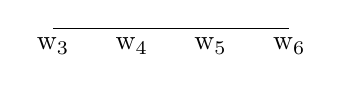
\begin{tikzpicture}
  \node (w3) at (0, 0) {w$_3$};
  \node (w4) at (1, 0) {w$_4$};
  \node (w5) at (2, 0) {w$_5$};
  \node (w6) at (3, 0) {w$_6$};
  \draw (w3.north) -- (w6.north);
\end{tikzpicture}\hfill\strut

\noindent
\parbox{4in}{
Or a span plus a point outside the span: \\
}\hfill\begin{tikzpicture}
  \node (w3) at (0, 0) {w$_3$};
  \node (w4) at (1, 0) {w$_4$};
  \node (w5) at (2, 0) {w$_5$};
  \node (w6) at (3, 0) {w$_6$};
  \node (w7) at (4, 0) {w$_7$};
  \node (w8) at (5, 0) {w$_8$};
  \draw (w3.north) -- (w6.north);
  \node [pointO] at (w8.north) {};
\end{tikzpicture}\hfill\strut

\noindent
\parbox[c]{2in}{
Whether a word in the item has edges, and whether the item can be modified to give it an edge, depends on its location: \\
}\hfill\begin{tabular}{lcrr}
  \hline
   & & Has & Can get \\
  Location & Example & edges? & edges? \\
  \hline
  \hline
  Within a span & w$_4$, w$_5$ & Yes & No \\
  At the ends of the span & w$_3$, w$_6$ & Maybe & Yes \\
  Between the span and & \multirow{2}{*}{w$_7$} & \multirow{2}{*}{No} & \multirow{2}{*}{No} \\
  the exterior point & & & \\
  At the exterior point & w$_8$ & Yes & Yes \\
  \hline \\
\end{tabular}\hfill\strut

\noindent
\parbox{4in}{
We start out with spans going between each pair of words, with no structure: \\
}\hfill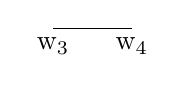
\begin{tikzpicture}
  \node (w3) at (0, 0) {w$_3$};
  \node (w4) at (1, 0) {w$_4$};
  \draw (w3.north) -- (w4.north);
\end{tikzpicture}\hfill\strut

\noindent
\parbox{2.5in}{
Our goal is to form a span that covers the entire sentence: \\
}\hfill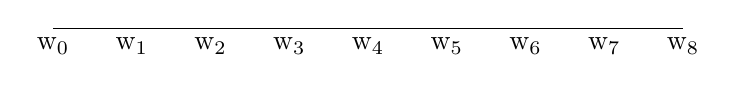
\begin{tikzpicture}
  \node (w0) at (0, 0) {w$_0$};
  \node (w1) at (1, 0) {w$_1$};
  \node (w2) at (2, 0) {w$_2$};
  \node (w3) at (3, 0) {w$_3$};
  \node (w4) at (4, 0) {w$_4$};
  \node (w5) at (5, 0) {w$_5$};
  \node (w6) at (6, 0) {w$_6$};
  \node (w7) at (7, 0) {w$_7$};
  \node (w8) at (8, 0) {w$_8$};
  \draw (w0.north) -- (w8.north);
\end{tikzpicture}

\noindent
\parbox{4in}{
For items that are just a span, we can create an edge between the endpoints.
An edge added like this is not crossed in the final, complete parse for the sentence. \\
}\hfill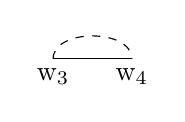
\begin{tikzpicture}
  \node (w3) at (0, 0) {w$_3$};
  \node (w4) at (1, 0) {w$_4$};
  \draw (w3.north) -- (w4.north);
  \draw [out=90,in=90,dashed] (w3.north) to (w4.north);
\end{tikzpicture}\hfill\strut

\noindent
\parbox{4in}{
For items with an exterior point we gain the option to create edges going between the exterior point and either end of the span.
In the top and middle cases, the edge being added will be crossed at some point later on in the derivation.
In the bottom case, the edge being added will cross one or more existing edges. \\
}\hfill\begin{minipage}{1.5in}
\begin{tikzpicture}
  \node (w3) at (0, 0) {w$_3$};
  \node (w4) at (1, 0) {w$_4$};
  \node (w5) at (2, 0) {w$_5$};
  \node (w6) at (3, 0) {w$_6$};
  \node (w7) at (4, 0) {w$_7$};
  \draw (w3.north) -- (w5.north);
  \node [pointO] at (w7.north) {};
  \draw [out=30,in=150,dashed] (w3.north) to (w7.north);
\end{tikzpicture} \\
\begin{tikzpicture}
  \node (w3) at (0, 0) {w$_3$};
  \node (w4) at (1, 0) {w$_4$};
  \node (w5) at (2, 0) {w$_5$};
  \node (w6) at (3, 0) {w$_6$};
  \node (w7) at (4, 0) {w$_7$};
  \draw (w3.north) -- (w5.north);
  \node [pointO] at (w7.north) {};
  \draw [out=50,in=130,dashed] (w5.north) to (w7.north);
\end{tikzpicture} \\
\begin{tikzpicture}
  \node (w3) at (0, 0) {w$_3$};
  \node (w4) at (1, 0) {w$_4$};
  \node (w5) at (2, 0) {w$_5$};
  \node (w6) at (3, 0) {w$_6$};
  \node (w7) at (4, 0) {w$_7$};
  \draw (w3.north) -- (w5.north);
  \node [pointO] at (w7.north) {};
  \draw [out=50,in=130,dashed] (w3.north) to (w5.north);
\end{tikzpicture} \\
\end{minipage}\hfill\strut

\noindent
\parbox{4in}{
The intuition for the deduction rules is that they combine two or three items with adjacent spans to create a new item.
By carefully deciding which combinations are permitted and which are not, we are able to provide guarantees about the final structure. \\
}\hfill\begin{minipage}{2.5in}
\strut\hfill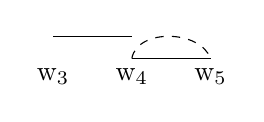
\begin{tikzpicture}
  \node (w3) at (0, 0) {w$_3$};
  \node (w4) at (1, 0) {w$_4$};
  \node (w5) at (2, 0) {w$_5$};
  \draw (0, 0.5) -- (1, 0.5);
  \draw (w4.north) -- (w5.north);
  \draw [out=80,in=110,dashed] (w4.north) to (w5.north);
\end{tikzpicture}\hfill\strut

\strut\hfill$\downarrow$\hfill\strut \\

\strut\hfill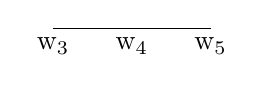
\begin{tikzpicture}
  \node (w3) at (0, 0) {w$_3$};
  \node (w4) at (1, 0) {w$_4$};
  \node (w5) at (2, 0) {w$_5$};
  \draw (w3.north) -- (w5.north);
\end{tikzpicture}\hfill\strut
\end{minipage}\hfill\strut

Crucially, the guarantees for the final structure can be made while only tracking certain properties of the sub-parts of the structure along the way.
That means for each item we can store just the max over sub-structures, rather than every individual sub-structure.
That in turn means that when creating a new item, we only consider how to combine these max-structures, not every structure.
As a result, the time complexity of our algorithm does not depend on the number of possible structures (exponential complexity), but instead on the number of possible items (polynomial complexity).

\subsection{Notation}

We use $p$, $q$, etc to refer to word positions.
To indicate ranges we use $[pq]$, $[pq)$, $(pq]$, or $(pq)$, where the bracket variations indicate inclusion, $[]$, or exclusion, $()$, of the endpoint.
To indicate an edge we use two points without brackets, \myeg $pq$.
To define a class of edges we either use a point and a set connected by a dash, \myeg $o$--$(pq)$, or two sets connected by a dash, \myeg $(ps)$--$(sq)$.

\subsection{Item Types} \label{sec:item-types-sketch}

As shown above and in Figure~\ref{fig:alg-example}, our items start and end on words, fully covering the gaps in between\footnote{
This is the inverse of the
conventional constituency parsing approach where items fully cover words and end in the gaps between words.
The idea can be traced back to \textcite{eisner:1996}.
}.
We use six item types, differing in the type of edge crossing they contain: \\

\strut\hfill\begin{tabular}{ll}
  \begin{tikzpicture}
    \node (p) at (0, 0) {$p$};
    \node (q) at (2, 0) {$q$};
    \draw (p.north) -- (q.north);
  \end{tikzpicture} &
  \parbox{0.70\textwidth}{
    \textbf{$I$, Interval}
    A span in which all points in $(pq)$ have a parent in $[pq]$, and no edges exist that go from outside $[pq]$ to points in $(pq)$. \\
  } \\
\end{tabular}\hfill\strut

\strut\hfill\begin{tabular}{ll}
  \begin{tikzpicture}
    \node (p) at (0, 0) {};
    \node (q) at (2, 0) {};
    \node (o) at (3, 0) {$o$};
    \node [pointO] at (o.north) {};
    \draw (p.north) -- (q.north);
    \draw [out=45,in=135] (p.north) to (o.north);
  \end{tikzpicture} &
  \parbox{0.70\textwidth}{
    \textbf{$X$, Exterval}
    An interval plus a single edge between $o$ and either $p$ or $q$, where $o$ is outside $[pq]$. \\
  } \\
\end{tabular}\hfill\strut

\strut\hfill\begin{tabular}{ll}
  \begin{tikzpicture}
    \node (p) at (0, 0) {};
    \node (m1) at (0.4, 0) {};
    \node (m2) at (0.8, 0) {};
    \node (m3) at (1.2, 0) {};
    \node (m4) at (1.6, 0) {};
    \node (q) at (2, 0) {};
    \node (o) at (3, 0) {};
    \draw (p.center) -- (q.center);
    \node [pointO] at (o.center) {};
    \draw [out=45,in=135] (m1.center) to (o.center);
    \draw [out=45,in=135] (m4.center) to (o.center);
    \draw [out=45,in=135] (p.center) to (m2.center);
    \draw [out=45,in=135] (m3.center) to (q.center);
  \end{tikzpicture} &
  \parbox{0.70\textwidth}{
    \textbf{$B$, Both}
    An interval $[pq]$ and a point $o$.
    $o$--$(pq)$ edge may be crossed by $p$--$(pq)$ or $q$--$(pq)$ edges, and at least one crossing of each type occurs.
    $o$--$(pq)$ edges may not be crossed by $(pq)$--$(pq)$ edges. \\
  } \\
\end{tabular}\hfill\strut

\strut\hfill\begin{tabular}{ll}
  \begin{tikzpicture}
    \node (p) at (0, 0) {};
    \node (m) at (0.6, 0) {};
    \node (m2) at (1.2, 0) {};
    \node (q) at (2, 0) {};
    \node (o) at (3, 0) {};
    \draw (p.center) -- (q.center);
    \node [pointO] at (o.center) {};
    \draw [out=45,in=135] (m.center) to (o.center);
    \draw [out=45,in=135] (p.center) to (m2.center);
  \end{tikzpicture} &
  \parbox{0.70\textwidth}{
    \textbf{$L$, Left}
    Same as $B$, but $o$--$(pq)$ edges may only be crossed by $p$--$(pq)$ edges. \\
  } \\
\end{tabular}\hfill\strut

\strut\hfill\begin{tabular}{ll}
  \begin{tikzpicture}
    \node (p) at (0, 0) {};
    \node (m) at (0.6, 0) {};
    \node (m2) at (1.2, 0) {};
    \node (q) at (2, 0) {};
    \node (o) at (3, 0) {};
    \draw (p.center) -- (q.center);
    \node [pointO] at (o.center) {};
    \draw [out=45,in=135] (m2.center) to (o.center);
    \draw [out=45,in=135] (m.center) to (q.center);
  \end{tikzpicture} &
  \parbox{0.70\textwidth}{
    \textbf{$R$, Right}
    Same as $L$, but with edges crossed by $q$--$(pq)$ edges rather than $p$-$(pq)$ edges. \\
  } \\
\end{tabular}\hfill\strut

\strut\hfill\begin{tabular}{ll}
  \begin{tikzpicture}
    \node (p) at (0, 0) {};
    \node (m) at (1, 0) {};
    \node (q) at (2, 0) {};
    \node (o) at (3, 0) {};
    \draw (p.center) -- (q.center);
    \node [pointO] at (o.center) {};
    \draw [out=45,in=135] (m.center) to (o.center);
  \end{tikzpicture} &
  \parbox{0.70\textwidth}{
    \textbf{$N$, Neither}
    An interval and a point, with a least one $o$--$(pq)$ edge.
    $o$--$(pq)$ edges can only be crossed by $pq$, not other $[pq]$--$[pq]$ edges. \\
  }
\end{tabular}\hfill\strut

\subsection{Example Derivation} \label{sec:example-derivation}

Figure~\ref{fig:alg-example} presents a derivation of a sentence with crossing edges, showing examples of several deduction rules.
We define the deduction rules in the next section from a top-down perspective to easily show how well they cover the space of structures.
To build intuition, here we describe the example bottom-up and with more conventional deductive reasoning notation. \\

\noindent
\parbox{4.5in}{
We initialize with items of width one, placing an item between each pair of words. \\
}\hfill\mbox{
  $\emptyset \; \mapsto \; I_{0,1}$
}

\noindent
\parbox{4.5in}{
Our main loop from Algorithm~\ref{alg:general-cky} considers each width and combines items, then adds structure.
We start with items of width one, which cannot be formed by combination.
We can add edges though, such as the \emph{We}--\emph{like} edge, and the \emph{like}--\emph{ROOT} edge.
Note, in the second case the edge creates an Exterval, and the edge will eventually be crossed. \\
}\hfill\parbox{1.5in}{
  $I_{1,2} \; \land \; pq_{1,2} \; \mapsto \; I_{1,2}$ \\
  $I_{0,1} \; \land \; po_{0,2} \; \mapsto \; X_{0,1}$ 
}

\noindent
\parbox{4.5in}{
In the next step we consider items of width two.
We can form an item of width two by combining items either side of \emph{to}: \\
}\hfill\mbox{
  $I_{2,3} \; \land \; I_{3,4} \; \mapsto \; I_{2,4}$
}

\noindent
\parbox{4.5in}{
From (3) to (4) we are still considering items of width two, but now adding edges, such as \emph{We}--\emph{run}.
This edge would not be part of a tree parse, and will be crossed in our complete parse: \\
}\hfill\mbox{
  $I_{2,4} \; \land \; po_{1,4} \; \mapsto \; X_{2,4}$ 
}

\noindent
\parbox{4.5in}{
Next, a width four item is formed by combining items either side of \emph{run}.
This creates a Neither item, as there is an uncrossed edge from the external point to within the span.
Note that we can determine it is an $N$ with only limited information about the internal structure of the items being combined. \\
}\hfill\mbox{
  $X_{2,4} \; \land \; I_{462} \; \mapsto \; N_{2,6}$
}

\noindent
\parbox{4.5in}{
Going from (5) to (6) we introduce our first crossing of edges.
The new edge, \emph{.}--\emph{like}, crosses the edge added two steps ago. \\
}\hfill\mbox{
  $N_{2,6} \; \land \; po_{2,6} \; \mapsto \; N_{2,4}$ 
}

\noindent
\parbox{4in}{
Finally, we combine three items to form the complete derivation. \\
}\hfill\mbox{
  $X_{0,1} \; \land \; I_{1,2} \land N_{2,6} \; \mapsto \; I_{0,6}$
}

\begin{figure}
\centering
\vspace{-5mm}

\tikzset{% 
  leftChild/.style={%
    ->,
    >=Stealth,
    shorten >=1pt,
    thin
  }
}

\tikzset{% 
  rightChild/.style={%
    <-,
    >=Stealth,
    shorten <=1pt,
    thin
  }
}

\tikzset{% 
  len1/.style={%
    out=30,
    in=150
  }
}

\tikzset{% 
  len2/.style={%
    out=32,
    in=148
  }
}

\tikzset{% 
  len3/.style={%
    out=34,
    in=146
  }
}

\tikzset{% 
  len4/.style={%
    out=34,
    in=146
  }
}
\tikzset{% 
  extPoint/.style={%
    fill=black,regular polygon, regular polygon sides=4,inner sep=0.75pt
  }
}
\tikzset{% 
  myGuide/.style={%
    densely dotted,
    thick,
    color=black!25
  }
}

\begin{tikzpicture}
  \pgfmathsetlength{\vertSmall}{7.5ex}
  \pgfmathsetlength{\vertBig}{9ex}

  \coordinate (offset) at (0.3, 0);
  \coordinate (voffset0) at (0, 0);
  \coordinate (voffset1) at (0, 0.05);

  \node (v0) at (0, 0) {};
  \node (w0) at (0, 0) {};
  \node (w1) at (2, 0) {};
  \node (w2) at (4, 0) {};
  \node (w3) at (6, 0) {};
  \node (w4) at (8, 0) {};
  \node (w5) at (10, 0) {};
  \node (w6) at (12, 0) {};

  \node (vA) [below=\vertBig of v0] {};
  \node (v1) [above=\vertSmall of v0] {};
  \node (v2) [above=\vertSmall of v1] {};
  \node (v3) [above=\vertSmall of v2] {};
  \node (v4) [above=\vertSmall of v3] {};
  \node (v5) [above=\vertSmall of v4] {};
  \node (v6) [above=\vertSmall of v5] {};

  \draw [myGuide] (w0 |- vA) -- (w0 |- v6);
  \draw [myGuide] (w1 |- vA) -- (w1 |- v6);
  \draw [myGuide] (w2 |- vA) -- (w2 |- v6);
  \draw [myGuide] (w3 |- vA) -- (w3 |- v2);
  \draw [myGuide] (w4 |- vA) -- (w4 |- v4);
  \draw [myGuide] (w5 |- vA) -- (w5 |- v2);
  \draw [myGuide] (w6 |- vA) -- (w6 |- v6);

  \node (w0text) [below=\vertBig of w0] {\strut ROOT};
  \node (w1text) [below=\vertBig of w1] {\strut We};
  \node (w2text) [below=\vertBig of w2] {\strut like};
  \node (w3text) [below=\vertBig of w3] {\strut to};
  \node (w4text) [below=\vertBig of w4] {\strut run};
  \node (w5text) [below=\vertBig of w5] {\strut fast};
  \node (w6text) [below=\vertBig of w6] {\strut .};

  \draw [rightChild,len2] ($(w0 |- vA) + (offset)$) to ($(w2 |- vA)$);
  \draw [leftChild,len1] ($(w1 |- vA) + (offset)$) to ($(w2 |- vA) - (offset) + (voffset0)$);
  \draw [leftChild,len1] ($(w3 |- vA) + (offset)$) to ($(w4 |- vA) - (offset) - (offset) + (voffset0)$);
  \draw [leftChild,len3] ($(w1 |- vA)$) to ($(w4 |- vA)$);
  \draw [rightChild,len2] ($(w2 |- vA) + (offset) + (voffset0)$) to ($(w4 |- vA) - (offset)$);
  \draw [rightChild,len1] ($(w4 |- vA) + (offset) + (voffset0)$) to ($(w5 |- vA) - (offset)$);
  \draw [rightChild,len4] ($(w2 |- vA)$) to ($(w6 |- vA) - (offset)$);

  \draw ($(w0) + (offset)$) -- node[at start,below=-2pt] {\small $\;$ I$_{0,1}$} ($(w1) - (offset)$);
  \draw ($(w1) + (offset)$) -- node[at start,below=-2pt] {\small $\;$ I$_{1,2}$} ($(w2) - (offset)$);
  \draw ($(w2) + (offset)$) -- node[at start,below=-2pt] {\small $\;$ I$_{2,3}$} ($(w3) - (offset)$);
  \draw ($(w3) + (offset)$) -- node[at start,below=-2pt] {\small $\;$ I$_{3,4}$} ($(w4) - (offset)$);
  \draw ($(w4) + (offset)$) -- node[at start,below=-2pt] {\small $\;$ I$_{4,5}$} ($(w5) - (offset)$);
  \draw ($(w5) + (offset)$) -- node[at start,below=-2pt] {\small $\;$ I$_{5,6}$} ($(w6) - (offset)$);
  \node [anchor=west] (step0) at (w6 |- v0) {\strut \small (1) Initialize};

  \draw ($(w0 |- v1) + (offset)$) -- node[at start,below=-2pt] {\small $\;$ X$_{0,1}$} ($(w1 |- v1) - (offset)$);
  \node [extPoint] at (w2 |- v1) {};
  \draw ($(w1 |- v1) + (offset)$) -- node[at start,below=-2pt] {\small $\;$ I$_{1,2}$} ($(w2 |- v1) - (offset)$);
  \draw ($(w3 |- v1) + (offset)$) -- node[at start,below=-2pt] {\small $\;$ I$_{3,4}$} ($(w4 |- v1) - (offset)$);
  \draw ($(w4 |- v1) + (offset)$) -- node[at start,below=-2pt] {\small $\;$ I$_{4,5}$} ($(w5 |- v1) - (offset)$);
  \draw [rightChild,len2] ($(w0 |- v1) + (offset)$) to ($(w2 |- v1) + (voffset1)$);
  \draw [leftChild,len1] ($(w1 |- v1) + (offset)$) to ($(w2 |- v1) - (offset) + (voffset0)$);
  \draw [leftChild,len1] ($(w3 |- v1) + (offset)$) to ($(w4 |- v1) - (offset) + (voffset0)$);
  \draw [rightChild,len1] ($(w4 |- v1) + (offset) + (voffset0)$) to ($(w5 |- v1) - (offset)$);
  \node [anchor=west] (step0) at (w6 |- v1) {\strut \small (2) Add edges};

  \draw ($(w2 |- v2) + (offset)$) -- node[at start,below=-2pt] {\small $\;$ I$_{2,4}$} ($(w4 |- v2) - (offset)$);
  \draw ($(w4 |- v2) + (offset)$) -- node[at start,below=-2pt] {\small $\;$ I$_{4,6}$} ($(w6 |- v2) - (offset)$);
  \draw [leftChild,len1] ($(w3 |- v2) + (offset)$) to ($(w4 |- v2) - (offset) + (voffset0)$);
  \draw [rightChild,len1] ($(w4 |- v2) + (offset) + (voffset0)$) to ($(w5 |- v2) - (offset)$);
  \node [anchor=west] (step0) at (w6 |- v2) {\strut \small (3) Combine};

  \draw ($(w2 |- v3) + (offset)$) -- node[at start,below=-2pt] {\small $\;$ X$_{2,4}$} ($(w4 |- v3) - (offset)$);
  \node [extPoint] at (w1 |- v3) {};
  \draw [leftChild,len1] ($(w3 |- v3) + (offset)$) to ($(w4 |- v3) - (offset) - (offset) + (voffset0)$);
  \draw [leftChild,len3] ($(w1 |- v3)$) to ($(w4 |- v3) + (voffset1) + (voffset1) - (offset)$);
  \draw [rightChild,len2] ($(w2 |- v3) + (offset) + (voffset0)$) to ($(w4 |- v3) - (offset)$);
  \node [anchor=west] (step0) at (w6 |- v3) {\strut \small (4) Add edges};

  \draw ($(w2 |- v4) + (offset)$) -- node[at start,below=-2pt] {\small $\;$ N$_{2,6}$} ($(w6 |- v4) - (offset)$);
  \node [extPoint] at (w1 |- v4) {};
  \draw [leftChild,len1] ($(w3 |- v4) + (offset)$) to ($(w4 |- v4) - (offset) - (offset) + (voffset0)$);
  \draw [leftChild,len3] ($(w1 |- v4)$) to ($(w4 |- v4)$);
  \draw [rightChild,len2] ($(w2 |- v4) + (offset) + (voffset0)$) to ($(w4 |- v4) - (offset)$);
  \draw [rightChild,len1] ($(w4 |- v4) + (offset) + (voffset0)$) to ($(w5 |- v4) - (offset)$);
  \node [anchor=west] (step0) at (w6 |- v4) {\strut \small (5) Combine};

  \draw ($(w2 |- v5) + (offset)$) -- node[at start,below=-2pt] {\small $\;$ N$_{2,6}$} ($(w6 |- v5) - (offset)$);
  \node [extPoint] at (w1 |- v5) {};
  \draw [leftChild,len1] ($(w3 |- v5) + (offset)$) to ($(w4 |- v5) - (offset) - (offset) + (voffset0)$);
  \draw [leftChild,len3] ($(w1 |- v5)$) to ($(w4 |- v5)$);
  \draw [rightChild,len2] ($(w2 |- v5) + (offset) + (voffset0)$) to ($(w4 |- v5) - (offset)$);
  \draw [rightChild,len1] ($(w4 |- v5) + (offset) + (voffset0)$) to ($(w5 |- v5) - (offset)$);
  \draw [rightChild,len4] ($(w2 |- v5) + (offset) + (voffset1) + (voffset1)$) to ($(w6 |- v5) - (offset)$);
  \node [anchor=west] (step0) at (w6 |- v5) {\strut \small (6) Add edges};

  \draw ($(w0 |- v6) + (offset)$) -- node[at start,below=-2pt] {\small $\;$ I$_{0,6}$} ($(w6 |- v6) - (offset)$);
  \draw [rightChild,len2] ($(w0 |- v6) + (offset)$) to ($(w2 |- v6) + (voffset1)$);
  \draw [leftChild,len1] ($(w1 |- v6) + (offset)$) to ($(w2 |- v6) - (offset) + (voffset0)$);
  \draw [leftChild,len1] ($(w3 |- v6) + (offset)$) to ($(w4 |- v6) - (offset) - (offset) + (voffset0)$);
  \draw [leftChild,len3] ($(w1 |- v6)$) to ($(w4 |- v6)$);
  \draw [rightChild,len2] ($(w2 |- v6) + (offset) + (voffset0)$) to ($(w4 |- v6) - (offset)$);
  \draw [rightChild,len1] ($(w4 |- v6) + (offset) + (voffset0)$) to ($(w5 |- v6) - (offset)$);
  \draw [rightChild,len4] ($(w2 |- v6)$) to ($(w6 |- v6) - (offset)$);
  \node [anchor=west] (step0) at (w6 |- v6) {\strut \small (7) Combine};
\end{tikzpicture}

\caption{\label{fig:alg-example}
An example derivation using our graph parsing deduction rules.
}
\end{figure}

\begin{landscape}
\begin{figure}
\newlength\spanWidth

\tikzstyle{question} = [rectangle, rounded corners, minimum width=3cm, minimum height=1cm,text centered, draw=black]
\tikzstyle{answer} = [thick,->,>=stealth]

\centering
\begin{tikzpicture}
  [every fit/.style={rectangle,rounded corners,draw,inner sep=2pt}]
  \pgfmathsetlength{\spanWidth}{2cm}

  \node (top) at (10,3) [question] {Item type?};

  \node (endX) at (6,0.2) {None needed};
  \node (endB) at (9,0.2) {Fig.~\ref{fig:rule-both}};
  \node (endN) at (12,0.2) {Fig.~\ref{fig:rule-neither}};
  \node [align=left] (endR) at (19,0.2) {Symmetric\\with L};

  \node (q1p) at (0, 0) {};
  \node (q1q) [right=\spanWidth of q1p] {};
  \node (q1t) at ($(q1p)!0.2!(q1q)$) {};
  \node (q1s) at ($(q1p)!0.5!(q1q)$) {};
  \node (q1a) at ($(q1p)!0.65!(q1q)$) {};
  \node (q1c) at ($(q1p)!0.35!(q1q)$) {};
  \node (q1b) at ($(q1p)!0.8!(q1q)$) {};
  \draw [thick] (q1p.center) -- (q1q.center);
  \draw [thick,out=60,in=120,color=white] (q1p.center) to node (q1pc) [midway] {} (q1c.center);
  \draw [thick,out=60,in=120,color=white] (q1t.center) to node (q1ta) [midway] {} (q1a.center);
  \draw [thick,out=60,in=120,color=white] (q1t.center) to node (q1tb) [midway] {} (q1b.center);
  \draw [very thick,out=60,in=120,color=blue,densely dashed] (q1p.center) to node (q1ps) [midway] {} (q1s.center);
  \node (q1) [fit=(q1p) (q1q) (q1ps) (q1pc) (q1ta) (q1tb)] {};

  \node (endIa) at (0,-1.8) {Fig.~\ref{fig:rule-interval-a}};

  \node (q2p) at (3, -2) {};
  \node (q2q) [right=\spanWidth of q2p] {};
  \node (q2t) at ($(q2p)!0.2!(q2q)$) {};
  \node (q2s) at ($(q2p)!0.5!(q2q)$) {};
  \node (q2a) at ($(q2p)!0.65!(q2q)$) {};
  \node (q2c) at ($(q2p)!0.35!(q2q)$) {};
  \node (q2b) at ($(q2p)!0.8!(q2q)$) {};
  \draw [thick] (q2p.center) -- (q2q.center);
  \draw [thick,out=60,in=120,color=white] (q2p.center) to node (q2pc) [midway] {} (q2c.center);
  \draw [thick,out=60,in=120,color=white] (q2t.center) to node (q2tb) [midway] {} (q2b.center);
  \draw [thick,out=60,in=120,color=black] (q2p.center) to node (q2ps) [midway] {} (q2s.center);
  \draw [very thick,out=60,in=120,color=blue,densely dashed] (q2t.center) to node (q2ta) [midway] {} (q2a.center);
  \node (q2) [fit=(q2p) (q2q) (q2ps) (q2pc) (q2ta) (q2tb)] {};

  \node (endIb) at (2,-3.8) {Fig.~\ref{fig:rule-interval-b}};

  \node (q3p) at (6, -4) {};
  \node (q3q) [right=\spanWidth of q3p] {};
  \node (q3t) at ($(q3p)!0.2!(q3q)$) {};
  \node (q3s) at ($(q3p)!0.5!(q3q)$) {};
  \node (q3a) at ($(q3p)!0.65!(q3q)$) {};
  \node (q3c) at ($(q3p)!0.35!(q3q)$) {};
  \node (q3b) at ($(q3p)!0.8!(q3q)$) {};
  \draw [thick] (q3p.center) -- (q3q.center);
  \draw [thick,out=60,in=120,color=white] (q3p.center) to node (q3pc) [midway] {} (q3c.center);
  \draw [thick,out=60,in=120,color=black] (q3p.center) to node (q3ps) [midway] {} (q3s.center);
  \draw [thick,out=60,in=120,color=black] (q3t.center) to node (q3ta) [midway] {} (q3a.center);
  \draw [very thick,out=60,in=120,color=blue,densely dashed] (q3t.center) to node (q3tb) [midway] {} (q3b.center);
  \node (q3) [fit=(q3p) (q3q) (q3ps) (q3pc) (q3ta) (q3tb)] {};

  \node (q4p) at (3, -6) {};
  \node (q4q) [right=\spanWidth of q4p] {};
  \node (q4t) at ($(q4p)!0.2!(q4q)$) {};
  \node (q4s) at ($(q4p)!0.5!(q4q)$) {};
  \node (q4a) at ($(q4p)!0.65!(q4q)$) {};
  \node (q4c) at ($(q4p)!0.35!(q4q)$) {};
  \node (q4b) at ($(q4p)!0.8!(q4q)$) {};
  \draw [thick] (q4p.center) -- (q4q.center);
  \draw [thick,out=60,in=120,color=white] (q4p.center) to node (q4pc) [midway] {} (q4c.center);
  \draw [thick,out=60,in=120,color=white] (q4t.center) to node (q4tb) [midway] {} (q4b.center);
  \draw [thick,out=60,in=120,color=black] (q4p.center) to node (q4ps) [midway] {} (q4s.center);
  \draw [thick,out=60,in=120,color=black] (q4t.center) to node (q4ta) [midway] {} (q4a.center);
  \draw [very thick,out=60,in=120,color=blue,densely dashed] (q4s.center) to node (q4sc) [midway] {} (q4b.center);
  \node (q4) [fit=(q4p) (q4q) (q4ps) (q4pc) (q4ta) (q4tb)] {};

  \node (endIc) at (2,-7.8) {Fig.~\ref{fig:rule-interval-c}};
  \node (endId) at (6,-7.8) {Fig.~\ref{fig:rule-interval-d}};

  \node (q5p) at (9, -6) {};
  \node (q5q) [right=\spanWidth of q5p] {};
  \node (q5t) at ($(q5p)!0.2!(q5q)$) {};
  \node (q5s) at ($(q5p)!0.5!(q5q)$) {};
  \node (q5a) at ($(q5p)!0.65!(q5q)$) {};
  \node (q5c) at ($(q5p)!0.35!(q5q)$) {};
  \node (q5b) at ($(q5p)!0.8!(q5q)$) {};
  \draw [thick] (q5p.center) -- (q5q.center);
  \draw [thick,out=60,in=120] (q5p.center) to node (q5ps) [midway] {} (q5s.center);
  \draw [thick,out=60,in=120] (q5t.center) to node (q5ta) [midway] {} (q5a.center);
  \draw [thick,out=60,in=120] (q5t.center) to node (q5tb) [midway] {} (q5b.center);
  \draw [very thick,out=60,in=120,color=blue,densely dashed] (q5p.center) to node (q5pc) [midway] {} (q5c.center);
  \node (q5) [fit=(q5p) (q5q) (q5ps) (q5pc) (q5ta) (q5tb)] {};

  \node (endIe) at (9,-7.8) {Fig.~\ref{fig:rule-interval-e}};
  \node (endIf) at (12,-7.8) {Fig.~\ref{fig:rule-interval-f}};

  \node (q6p) at (14, 0) {};
  \node (q6q) [right=0.7\spanWidth of q6p] {};
  \node (q6x) [right=\spanWidth of q6p] {};
  \node [pointO] at (q6x) {};
  \node (q6a) at ($(q6p)!0.2!(q6q)$) {};
  \node (q6b) at ($(q6p)!0.4!(q6q)$) {};
  \node (q6s) at ($(q6p)!0.6!(q6q)$) {};
  \node (q6c) at ($(q6p)!0.8!(q6q)$) {};
  \draw [thick] (q6p.center) -- (q6q.center);
  \draw [thick,out=60,in=120,color=white] (q6b.center) to node (q6bx) [midway] {} (q6x.center);
  \draw [thick,out=60,in=120] (q6p.center) to node (q6ps) [midway] {} (q6s.center);
  \draw [thick,out=60,in=120] (q6a.center) to node (q6ax) [midway] {} (q6x.center);
  \draw [very thick,out=60,in=120,color=blue,densely dashed] (q6c.center) to node (q6cx) [midway] {} (q6x.center);
  \node (q6) [fit=(q6p) (q6q) (q6x) (q6ps) (q6ax) (q6bx) (q6cx)] {};

  \node (endLc) at (17,-1.8) {Fig.~\ref{fig:rule-left-c}};

  \node (q7p) at (12, -2) {};
  \node (q7q) [right=0.7\spanWidth of q7p] {};
  \node (q7x) [right=\spanWidth of q7p] {};
  \node [pointO] at (q7x) {};
  \node (q7a) at ($(q7p)!0.2!(q7q)$) {};
  \node (q7b) at ($(q7p)!0.4!(q7q)$) {};
  \node (q7s) at ($(q7p)!0.6!(q7q)$) {};
  \node (q7c) at ($(q7p)!0.8!(q7q)$) {};
  \draw [thick] (q7p.center) -- (q7q.center);
  \draw [thick,out=60,in=120,color=white] (q7c.center) to node (q7cx) [midway] {} (q7x.center);
  \draw [thick,out=60,in=120] (q7p.center) to node (q7ps) [midway] {} (q7s.center);
  \draw [thick,out=60,in=120] (q7a.center) to node (q7ax) [midway] {} (q7x.center);
  \draw [very thick,out=60,in=120,color=blue,densely dashed] (q7b.center) to node (q7bx) [midway] {} (q7x.center);
  \node (q7) [fit=(q7p) (q7q) (q7x) (q7ps) (q7ax) (q7bx) (q7cx)] {};

  \node (endLa) at (11,-3.8) {Fig.~\ref{fig:rule-left-a}};
  \node (endLb) at (15,-3.8) {Fig.~\ref{fig:rule-left-b}};

  \draw [answer] (q1) -- node [midway,left=4pt] {Yes} (q2);
  \draw [answer] (q1) -- node [midway,left=4pt] {No} (endIa);
  \draw [answer] (q2) -- node [midway,left=4pt] {Yes} (q3);
  \draw [answer] (q2) -- node [midway,left=4pt] {No} (endIb);
  \draw [answer] (q3) -- node [midway,left=4pt] {No} (q4);
  \draw [answer] (q3) -- node [midway,left=4pt] {Yes} (q5);
  \draw [answer] (q4) -- node [midway,left=4pt] {No} (endIc);
  \draw [answer] (q4) -- node [midway,left=4pt] {Yes} (endId);
  \draw [answer] (q5) -- node [midway,left=4pt] {No} (endIe);
  \draw [answer] (q5) -- node [midway,left=4pt] {Yes} (endIf);
  \draw [answer] (top) -- node [midway,left=22pt] {I} (q1);
  \draw [answer] (top) -- node [midway,left=8pt] {X} (endX);
  \draw [answer] (top) -- node [midway,left=4pt] {B} (endB);
  \draw [answer] (top) -- node [midway,right=8pt] {L} (q6);
  \draw [answer] (top) -- node [midway,right=14pt] {R} (endR);
  \draw [answer] (q6) -- node [midway,left=4pt] {No} (q7);
  \draw [answer] (top) -- node [midway,right=4pt] {N} (endN);
  \draw [answer] (q7) -- node [midway,left=4pt] {No} (endLa);
  \draw [answer] (q7) -- node [midway,left=4pt] {Yes} (endLb);
  \draw [answer] (q6) -- node [midway,left=4pt] {Yes} (endLc);

\end{tikzpicture}
\caption[Overall picture of deduction rule definitions.]{\label{fig:deduction-defs}
Our algorithm defines a unique decomposition for any structure.
This chart shows how we define the decompositions that involve multiple items (as opposed to removing a single edge, such as in $X$ cases).
Each rectangle poses a questions, using the black structure to express what is known, and the dashed blue edge to ask the question: is such an edge present or not?
Leaves of the chart are labeled with the section in the text that gives the decomposition for that case.
}
\end{figure}

\end{landscape}

\subsection{Deduction Rules} \label{sec:deduction-rules-sketch}

\newlength{\deductionCaptionLength}
\newlength{\deductionRuleLength}
\setlength{\deductionCaptionLength}{0.35\textwidth}
\setlength{\deductionRuleLength}{0.95\textwidth}

One set of deduction rules is concerned with removing direct edges between the points $p$, $q$, and $o$ in each item.
These are straightforward, so we leave them for the full derivation in Section~\ref{sec:full-algorithm}.
The other type of deduction rules, which we sketch below, involve decomposing an item into parts.

To make the deduction rules manageable, we define some constraints explicitly, and then use code to enumerate all options and enforce additional constraints.
Here we describe the explicit constraints and the reasoning behind them.

When parsing, we simply have a list of valid rules and consider any way of combining items that satisfies a rule.
To define the rules, we need to consider each of our item types and define a unique decomposition into smaller pieces.
Figure~\ref{fig:deduction-defs} gives an overview of how this process works.
For some item types, such as $X$, every possible structure can be broken down into pieces in the same way.
For others, such as $L$, how the item is broken down depends on some properties of its structure.
Below we work through each path in Figure~\ref{fig:deduction-defs}, specifying the questions more precisely and then providing the decomposition.

\subsubsection{Interval}\label{sec:interval}
Is there a $p$--$(pq)$ edge? \\
No, then split at $p+1$: \\

\noindent
\begin{minipage}{\deductionRuleLength}
\centering
\hfill\begin{tikzpicture}
  \pgfmathsetlength{\vertSmall}{2ex}
  \pgfmathsetlength{\labelGap}{1ex}
  \pgfmathsetlength{\coordGap}{-0.5ex}
  \node (hlref) at (0, 0) {};
  \node (hmref) at (1, 0) {};
  \node (hrref) at (4, 0) {};

  \node (p0) at (hlref) {};
  \node (s0a) at (hmref) {};
  \node (v0bref) [below=\vertSmall of p0.center] {};
  \node (s0b) at (v0bref -| hmref) {};
  \node (q0) at (v0bref -| hrref) {};
  \node (label0) [left=\labelGap of p0] {$I$};
  \node (label0) [left=\labelGap of v0bref] {$I$};
  \draw (p0.center) -- (s0a.center);
  \draw (s0b.center) -- (q0.center);

  \node (lb) at (v0bref -| hlref) {};
  \node (sb) at (v0bref -| hmref) {};
  \node (rb) at (v0bref -| hrref) {};
  \node (ltext) [below=\coordGap of lb.center] {\small \strut $p$};
  \node (stext) [below=\coordGap of sb.center] {\small \strut ${p+1}$};
  \node (rtext) [below=\coordGap of rb.center] {\small \strut $q$};
\end{tikzpicture}\hfill
\raisebox{4mm}{\parbox[b]{\deductionCaptionLength}{\captionof{figure}{\label{fig:rule-interval-a} Deduction rule $I_0$}}}
\end{minipage}
\vspace{5mm}

\noindent
Yes, then consider $ps$, the longest $p$--$(pq)$ edge. \\
Do any edges cross $ps$? \\
No, then split at $s$: \\

\noindent
\begin{minipage}{\deductionRuleLength}
\centering
\hfill\begin{tikzpicture}
  \pgfmathsetlength{\vertSmall}{2ex}
  \pgfmathsetlength{\labelGap}{1ex}
  \pgfmathsetlength{\coordGap}{-0.5ex}
  \node (hlref) at (0, 0) {};
  \node (hmref) at (2, 0) {};
  \node (hrref) at (4, 0) {};

  \node (p0) at (hlref) {};
  \node (s0a) at (hmref) {};
  \node (v0bref) [below=\vertSmall of p0.center] {};
  \node (s0b) at (v0bref -| hmref) {};
  \node (q0) at (v0bref -| hrref) {};
  \node (label0) [left=\labelGap of p0] {$I$};
  \node (label0) [left=\labelGap of v0bref] {$I$};
  \draw (p0.center) -- (s0a.center);
  \draw (s0b.center) -- (q0.center);
  \draw [required,out=30,in=150] (p0.center) to (s0a.center);

  \node (lb) at (v0bref -| hlref) {};
  \node (sb) at (v0bref -| hmref) {};
  \node (rb) at (v0bref -| hrref) {};
  \node (ltext) [below=\coordGap of lb.center] {\small \strut $p$};
  \node (stext) [below=\coordGap of sb.center] {\small \strut $s$};
  \node (rtext) [below=\coordGap of rb.center] {\small \strut $q$};
\end{tikzpicture}\hfill
\raisebox{4mm}{\parbox[b]{\deductionCaptionLength}{\captionof{figure}{\label{fig:rule-interval-b} Deduction rule $I_1$}}}
\end{minipage}
\vspace{5mm}

\noindent
Yes, then consider the set of edges $C$, that cross $ps$.
If $|C| > 1$, let $t$ be the common endpoint of all edges in $C$ (they must have a common endpoint to satisfy the \oneEC property for $ps$).
If $|C| = 1$, let $t$ be the endpoint outside $ps$.

\noindent
Is $s < t$ and are there any $s$--$(tq)$ edges? \\
Yes to both: \\

\noindent
\begin{minipage}{\deductionRuleLength}
\centering
\hfill\begin{tikzpicture}
  \pgfmathsetlength{\vertSmall}{2ex}
  \pgfmathsetlength{\labelGap}{1ex}
  \pgfmathsetlength{\coordGap}{-0.5ex}
  \node (l) at (0, 0) {};
  \node (ls) at (0.5, 0) {};
  \node (s) at (1.5, 0) {};
  \node (t) at (2.5, 0) {};
  \node (tr) at (3.5, 0) {};
  \node (r) at (4, 0) {};

  \node (v0) at (l) {};
  \node (p0) at (v0 -| l) {};
  \node (q0) at (v0 -| s) {};
  \node (o0) at (v0 -| t) {};
  \node [pointO] at (o0) {};
  \node (label0) [left=\labelGap of v0] {$R$ or $N$};
  \node (v1) [below=\vertSmall of v0.center] {};
  \node (p1) at (v1 -| s) {};
  \node (q1) at (v1 -| t) {};
  \node (label1) [left=\labelGap of v1] {$I$};
  \node (v2) [below=\vertSmall of v1.center] {};
  \node (p2) at (v2 -| t) {};
  \node (q2) at (v2 -| r) {};
  \node (o2) at (v2 -| s) {};
  \node [pointO] at (o2) {};
  \node (label2) [left=\labelGap of v2] {$L$, $N$ or $X$};
  \draw (p0.center) -- (q0.center);
  \draw (p1.center) -- (q1.center);
  \draw (p2.center) -- (q2.center);
  \draw [required,out=30,in=150] (p0.center) to (q0.center);
  \draw [required,out=150,in=30] (o0.center) to (v0 -| ls);
  \draw [required,out=30,in=150] (o2.center) to (v2 -| tr);

  \node (lb) at (v2 -| l) {};
  \node (tb) at (v2 -| t) {};
  \node (sb) at (v2 -| s) {};
  \node (rb) at (v2 -| r) {};
  \node (ltext) [below=\coordGap of lb.center] {\small \strut $p$};
  \node (ttext) [below=\coordGap of tb.center] {\small \strut $t$};
  \node (stext) [below=\coordGap of sb.center] {\small \strut $s$};
  \node (rtext) [below=\coordGap of rb.center] {\small \strut $q$};
\end{tikzpicture}\hfill
\raisebox{4mm}{\parbox[b]{\deductionCaptionLength}{\captionof{figure}{\label{fig:rule-interval-d} Deduction rule $I_2$}}}
\end{minipage}
\vspace{5mm}

\noindent
Yes $s < t$, no $s$--$(tq)$ edges (in this case it is also possible that $t = q$, in which case there is no $[tq]$ item): \\

\noindent
\begin{minipage}{\deductionRuleLength}
\centering
\hfill\begin{tikzpicture}
  \pgfmathsetlength{\vertSmall}{2ex}
  \pgfmathsetlength{\labelGap}{1ex}
  \pgfmathsetlength{\coordGap}{-0.5ex}
  \node (l) at (0, 0) {};
  \node (ls) at (0.5, 0) {};
  \node (s) at (1.5, 0) {};
  \node (t) at (2.5, 0) {};
  \node (tr) at (3.5, 0) {};
  \node (r) at (4, 0) {};

  \node (v0) at (l) {};
  \node (p0) at (v0 -| l) {};
  \node (q0) at (v0 -| s) {};
  \node (o0) at (v0 -| t) {};
  \node [pointO] at (o0) {};
  \node (label0) [left=\labelGap of v0] {$B$, $L$, $R$ or $N$};
  \node (v1) [below=\vertSmall of v0.center] {};
  \node (p1) at (v1 -| s) {};
  \node (q1) at (v1 -| t) {};
  \node (label1) [left=\labelGap of v1] {$I$};
  \node (v2) [below=\vertSmall of v1.center] {};
  \node (p2) at (v2 -| t) {};
  \node (q2) at (v2 -| r) {};
  \node (label2) [left=\labelGap of v2] {$I$};
  \draw (p0.center) -- (q0.center);
  \draw (p1.center) -- (q1.center);
  \draw (p2.center) -- (q2.center);
  \draw [required,out=30,in=150] (p0.center) to (q0.center);
  \draw [required,out=150,in=30] (o0.center) to (v0 -| ls);

  \node (lb) at (v2 -| l) {};
  \node (tb) at (v2 -| t) {};
  \node (sb) at (v2 -| s) {};
  \node (rb) at (v2 -| r) {};
  \node (ltext) [below=\coordGap of lb.center] {\small \strut $p$};
  \node (ttext) [below=\coordGap of tb.center] {\small \strut $t$};
  \node (stext) [below=\coordGap of sb.center] {\small \strut $s$};
  \node (rtext) [below=\coordGap of rb.center] {\small \strut $q$};
\end{tikzpicture}\hfill
\raisebox{4mm}{\parbox[b]{\deductionCaptionLength}{\captionof{figure}{\label{fig:rule-interval-c} Deduction rule $I_3$}}}
\end{minipage}
\vspace{5mm}

\noindent
Now consider $s > t$.
In this case $C > 1$ by construction.
Are there any $p$--$(ts)$ edges? \\
Yes: \\

\noindent
\begin{minipage}{\deductionRuleLength}
\centering
\hfill\begin{tikzpicture}
  \pgfmathsetlength{\vertSmall}{2ex}
  \pgfmathsetlength{\labelGap}{1ex}
  \pgfmathsetlength{\coordGap}{-0.5ex}
  \node (l) at (0, 0) {};
  \node (t) at (1.5, 0) {};
  \node (ts) at (2, 0) {};
  \node (s) at (2.5, 0) {};
  \node (sr1) at (3, 0) {};
  \node (sr2) at (3.5, 0) {};
  \node (r) at (4, 0) {};

  \node (v0) at (l) {};
  \node (p0) at (v0 -| l) {};
  \node (q0) at (v0 -| t) {};
  \node (label0) [left=\labelGap of v0] {$I$};
  \node (v1) [below=\vertSmall of v0.center] {};
  \node (p1) at (v1 -| t) {};
  \node (q1) at (v1 -| s) {};
  \node (o1) at (v1 -| p) {};
  \node [pointO] at (o1) {};
  \node (label1) [left=\labelGap of v1] {$L$ or $N$};
  \node (v2) [below=\vertSmall of v1.center] {};
  \node (p2) at (v2 -| s) {};
  \node (q2) at (v2 -| r) {};
  \node (o2) at (v2 -| t) {};
  \node [pointO] at (o2) {};
  \node (label2) [left=\labelGap of v2] {$N$};
  \draw (p0.center) -- (q0.center);
  \draw (p1.center) -- (q1.center);
  \draw (p2.center) -- (q2.center);
  \draw [required,out=30,in=150] (o1.center) to (q1.center);
  \draw [required,out=30,in=150] (o1.center) to (v1 -| ts);
  \draw [required,out=30,in=150] (o2.center) to (v2 -| sr1);
  \draw [required,out=30,in=150] (o2.center) to (v2 -| sr2);

  \node (lb) at (v2 -| l) {};
  \node (tb) at (v2 -| t) {};
  \node (sb) at (v2 -| s) {};
  \node (rb) at (v2 -| r) {};
  \node (ltext) [below=\coordGap of lb.center] {\small \strut $p$};
  \node (ttext) [below=\coordGap of tb.center] {\small \strut $t$};
  \node (stext) [below=\coordGap of sb.center] {\small \strut $s$};
  \node (rtext) [below=\coordGap of rb.center] {\small \strut $q$};
\end{tikzpicture}\hfill
\raisebox{4mm}{\parbox[b]{\deductionCaptionLength}{\captionof{figure}{\label{fig:rule-interval-f} Deduction rule $I_4$}}}
\end{minipage}
\vspace{5mm}

\noindent
No: \\

\noindent
\begin{minipage}{\deductionRuleLength}
\centering
\hfill\begin{tikzpicture}
  \pgfmathsetlength{\vertSmall}{2ex}
  \pgfmathsetlength{\labelGap}{1ex}
  \pgfmathsetlength{\coordGap}{-0.5ex}
  \node (l) at (0, 0) {};
  \node (t) at (1.5, 0) {};
  \node (ts) at (2, 0) {};
  \node (s) at (2.5, 0) {};
  \node (sr1) at (3, 0) {};
  \node (sr2) at (3.5, 0) {};
  \node (r) at (4, 0) {};

  \node (v0) at (l) {};
  \node (p0) at (v0 -| l) {};
  \node (q0) at (v0 -| t) {};
  \node (o0) at (v0 -| s) {};
  \node [pointO] at (o0) {};
  \node (label0) [left=\labelGap of v0] {$R$, $N$ or $X$};
  \node (v1) [below=\vertSmall of v0.center] {};
  \node (p1) at (v1 -| t) {};
  \node (q1) at (v1 -| s) {};
  \node (label1) [left=\labelGap of v1] {$I$};
  \node (v2) [below=\vertSmall of v1.center] {};
  \node (p2) at (v2 -| s) {};
  \node (q2) at (v2 -| r) {};
  \node (o2) at (v2 -| t) {};
  \node [pointO] at (o2) {};
  \node (label2) [left=\labelGap of v2] {$N$};
  \draw (p0.center) -- (q0.center);
  \draw (p1.center) -- (q1.center);
  \draw (p2.center) -- (q2.center);
  \draw [required,out=30,in=150] (p0.center) to (o0.center);
  \draw [required,out=30,in=150] (o2.center) to (v2 -| sr1);
  \draw [required,out=30,in=150] (o2.center) to (v2 -| sr2);

  \node (lb) at (v2 -| l) {};
  \node (tb) at (v2 -| t) {};
  \node (sb) at (v2 -| s) {};
  \node (rb) at (v2 -| r) {};
  \node (ltext) [below=\coordGap of lb.center] {\small \strut $p$};
  \node (ttext) [below=\coordGap of tb.center] {\small \strut $t$};
  \node (stext) [below=\coordGap of sb.center] {\small \strut $s$};
  \node (rtext) [below=\coordGap of rb.center] {\small \strut $q$};
\end{tikzpicture}\hfill
\raisebox{4mm}{\parbox[b]{\deductionCaptionLength}{\captionof{figure}{\label{fig:rule-interval-e} Deduction rule $I_5$}}}
\end{minipage}
\vspace{5mm}

\subsubsection{Exterval} \label{sec:alg:exterval}
No decomposition rules are needed, as the removal of the $op$ or $oq$ edge leaves behind an Interval.

\subsubsection{Both} \label{sec:alg:both}
Consider the case when $o$ is to the right (the case when $o$ is to the left is symmetrical).
Consider $ps_p$, the longest $p$--$(pq)$ edge. \\
Does $ps_p$ cross any $q$--$(pq)$ edges? \\
Yes: \\

\noindent
\begin{minipage}{\deductionRuleLength}
\centering
\hfill\begin{tikzpicture}
  \pgfmathsetlength{\vertSmall}{2ex}
  \pgfmathsetlength{\labelGap}{1ex}
  \pgfmathsetlength{\coordGap}{-0.5ex}
  \node (l) at (0, 0) {};
  \node (t) at (1.5, 0) {};
  \node (ts) at (2, 0) {};
  \node (s) at (2.5, 0) {};
  \node (sr1) at (3, 0) {};
  \node (sr2) at (3.5, 0) {};
  \node (r) at (4, 0) {};
  \node (o) at (5, 0) {};

  \node (v0) at (l) {};
  \node (p0) at (v0 -| l) {};
  \node (q0) at (v0 -| t) {};
  \node (o0) at (v0 -| s) {};
  \node [pointO] at (o0) {};
  \node (label0) [left=\labelGap of v0] {$R$, $N$ or $X$};
  \node (v1) [below=\vertSmall of v0.center] {};
  \node (p1) at (v1 -| t) {};
  \node (q1) at (v1 -| s) {};
  \node (o1) at (v1 -| o) {};
  \node [pointO] at (o1) {};
  \node (label1) [left=\labelGap of v1] {$X'$};
  \node (v2) [below=\vertSmall of v1.center] {};
  \node (p2) at (v2 -| s) {};
  \node (q2) at (v2 -| r) {};
  \node (o2) at (v2 -| t) {};
  \node [pointO] at (o2) {};
  \node (label2) [left=\labelGap of v2] {$L$, $N$ or $X$};
  \draw (p0.center) -- (q0.center);
  \draw (p1.center) -- (q1.center);
  \draw (p2.center) -- (q2.center);
  \draw [required,out=30,in=150] (p0.center) to (o0.center);
  \draw [required,out=30,in=150] (o2.center) to (q2.center);
  \draw [required,out=20,in=160] (p1.center) to (o1.center);
  \draw [required,out=20,in=160] (q1.center) to (o1.center);

  \node (lb) at (v2 -| l) {};
  \node (tb) at (v2 -| t) {};
  \node (sb) at (v2 -| s) {};
  \node (rb) at (v2 -| r) {};
  \node (ob) at (v2 -| o) {};
  \node (ltext) [below=\coordGap of lb.center] {\small \strut $p$};
  \node (ttext) [below=\coordGap of tb.center] {\small \strut $s_p$};
  \node (stext) [below=\coordGap of sb.center] {\small \strut $s_q$};
  \node (rtext) [below=\coordGap of rb.center] {\small \strut $q$};
  \node (otext) [below=\coordGap of ob.center] {\small \strut $o$};
\end{tikzpicture}\hfill
\raisebox{4mm}{\parbox[b]{\deductionCaptionLength}{\captionof{figure}{\label{fig:rule-both-fail-a} Excluded $B$ deduction rule}}}
\end{minipage}
\vspace{5mm}

The extra edges shown must be present because of the definition of $B$ items and the \oneEC property.
The $X'$ is a slight variation on our $X$, since it has both $s_qo$ and $s_po$.
We do not include this rule because it would be $O(n^5)$, and this specific structure is almost never observed in the treebank.

\noindent
Now consider the alternative, when $ps_p$ does not cross any $q$--$(pq)$ edges.
In this case the possibilities follow a pattern: \\

\noindent
\begin{minipage}{\deductionRuleLength}
\centering
\hfill\parbox{3in}{
\begin{tikzpicture}
  \node (p) at (1, 0) {};
  \node (m0) at (1.5, 0) {};
  \node (sp) at (2, 0) {};
  \node (sq) at (4, 0) {};
  \node (m1) at (4.5, 0) {};
  \node (q) at (5, 0) {};
  \node (o) at (6, 0) {};
  \node [pointO] at (o.north) {};
  \draw (p.north) -- (q.north);
  \draw [out=45,in=135] (p.north) to (sp.north);
  \draw [out=45,in=135] (sq.north) to (q.north);
  \draw [out=20,in=160] (m0.north) to (o.north);
  \draw [out=20,in=160] (m1.north) to (o.north);
\end{tikzpicture} \\
\begin{tikzpicture}
  \node (p) at (1, 0) {};
  \node (m0) at (1.5, 0) {};
  \node (sp) at (2, 0) {};
  \node (m2) at (2.5, 0) {};
  \node (sq) at (4, 0) {};
  \node (m1) at (4.5, 0) {};
  \node (q) at (5, 0) {};
  \node (o) at (6, 0) {};
  \node [pointO] at (o.north) {};
  \draw (p.north) -- (q.north);
  \draw [out=45,in=135] (p.north) to (sp.north);
  \draw [out=45,in=135] (sq.north) to (q.north);
  \draw [out=25,in=155] (m0.north) to (m2.north);
  \draw [out=20,in=160] (m0.north) to (o.north);
  \draw [out=20,in=160] (m1.north) to (o.north);
\end{tikzpicture} \\
\begin{tikzpicture}
  \node (p) at (1, 0) {};
  \node (m0) at (1.5, 0) {};
  \node (s) at (2, 0) {};
  \node (m2) at (2.5, 0) {};
  \node (m3) at (3, 0) {};
  \node (sq) at (4, 0) {};
  \node (m1) at (4.5, 0) {};
  \node (q) at (5, 0) {};
  \node (o) at (6, 0) {};
  \node [pointO] at (o.north) {};
  \draw (p.north) -- (q.north);
  \draw [out=45,in=135] (p.north) to (s.north);
  \draw [out=45,in=135] (sq.north) to (q.north);
  \draw [out=25,in=155] (m0.north) to (m2.north);
  \draw [out=20,in=160] (m0.north) to (o.north);
  \draw [out=20,in=160] (m1.north) to (o.north);
  \draw [out=25,in=155] (s.north) to (m3.north);
\end{tikzpicture} \\
\begin{tikzpicture}
  \node (p) at (1, 0) {};
  \node (m0) at (1.5, 0) {};
  \node (s) at (2, 0) {};
  \node (m2) at (2.5, 0) {};
  \node (m3) at (3, 0) {};
  \node (m4) at (3.5, 0) {};
  \node (sq) at (4, 0) {};
  \node (m1) at (4.5, 0) {};
  \node (q) at (5, 0) {};
  \node (o) at (6, 0) {};
  \node [pointO] at (o.north) {};
  \draw (p.north) -- (q.north);
  \draw [out=45,in=135] (p.north) to (s.north);
  \draw [out=45,in=135] (sq.north) to (q.north);
  \draw [out=25,in=155] (m0.north) to (m2.north);
  \draw [out=20,in=160] (m0.north) to (o.north);
  \draw [out=20,in=160] (m1.north) to (o.north);
  \draw [out=25,in=155] (s.north) to (m3.north);
  \draw [out=25,in=155] (m2.north) to (m4.north);
\end{tikzpicture} \\
\begin{tikzpicture}
  \node (p) at (1, 0) {};
  \node (m0) at (1.5, 0) {};
  \node (s) at (2, 0) {};
  \node (m2) at (2.5, 0) {};
  \node (m3) at (3, 0) {};
  \node (m4) at (3.5, 0) {};
  \node (sq) at (4, 0) {};
  \node (m1) at (4.5, 0) {};
  \node (q) at (5, 0) {};
  \node (o) at (6, 0) {};
  \node [pointO] at (o.north) {};
  \draw [out=45,in=135] (p.north) to (s.north);
  \draw [out=45,in=135] (sq.north) to (q.north);
  \draw [out=25,in=155] (m0.north) to (m2.north);
  \draw [out=20,in=160] (m0.north) to (o.north);
  \draw [out=20,in=160] (m1.north) to (o.north);
  \draw [out=25,in=155] (s.north) to (m3.north);
  \draw [out=25,in=155] (m2.north) to (m4.north);
  \draw [out=25,in=155] (m4.north) to (m1.north);
  \draw [out=25,in=155] (m3.north) to (sq.north);
  \node [fill=white] (dots) at (3,0.25) {\small . . .};
  \draw (p.north) -- (q.north);
\end{tikzpicture}
}\hfill
\raisebox{4mm}{\parbox[b]{\deductionCaptionLength}{\captionof{figure}{\label{fig:rule-both-fail-b} $B$ structural pattern}}}
\end{minipage}
\vspace{5mm}

Does the pattern go all the way to the right, as shown in the last case? \\
Yes:

\begin{center}
\parbox{0.65\textwidth}{
We cannot define a simple decomposition of the structure using our item types.
By eliminating this case we restrict ourselves to a subset of one-endpoint-crossing graphs.
This does not decrease treebank coverage. \\
}
\end{center}

\noindent
No, then use the end of the edge crossing pattern as $s$ and decompose the item as: \\

\noindent
\begin{minipage}{\deductionRuleLength}
\centering
\hfill\begin{tikzpicture}
  \pgfmathsetlength{\vertSmall}{2ex}
  \pgfmathsetlength{\labelGap}{1ex}
  \pgfmathsetlength{\coordGap}{-0.5ex}
  \node (l) at (0, 0) {};
  \node (ls) at (1, 0) {};
  \node (s) at (2, 0) {};
  \node (sr) at (3, 0) {};
  \node (r) at (4, 0) {};
  \node (o) at (5, 0) {};

  \node (v0) at (l) {};
  \node (p0) at (v0 -| l) {};
  \node (q0) at (v0 -| s) {};
  \node (o0) at (v0 -| o) {};
  \node [pointO] at (o0) {};
  \node (label0) [left=\labelGap of v0] {$L$ or $N$};
  \node (v1) [below=\vertSmall of v0.center] {};
  \node (p1) at (v1 -| s) {};
  \node (q1) at (v1 -| r) {};
  \node (o1) at (v1 -| o) {};
  \node [pointO] at (o1) {};
  \node (label1) [left=\labelGap of v1] {$R$ or $N$};
  \draw (p0.center) -- (q0.center);
  \draw (p1.center) -- (q1.center);
  \draw [optional,out=30,in=150] (p0.center) to (q0.center);
  \draw [optional,out=30,in=150] (p1.center) to (q1.center);
  \draw [required,out=20,in=160] (v0 -| ls) to (o0.center);
  \draw [required,out=30,in=150] (v1 -| sr) to (o1.center);

  \node (lb) at (v1 -| l) {};
  \node (sb) at (v1 -| s) {};
  \node (rb) at (v1 -| r) {};
  \node (ob) at (v1 -| o) {};
  \node (ltext) [below=\coordGap of lb.center] {\small \strut $p$};
  \node (stext) [below=\coordGap of sb.center] {\small \strut $s$};
  \node (rtext) [below=\coordGap of rb.center] {\small \strut $q$};
  \node (otext) [below=\coordGap of ob.center] {\small \strut $o$};
\end{tikzpicture}\hfill
\raisebox{4mm}{\parbox[b]{\deductionCaptionLength}{\captionof{figure}{\label{fig:rule-both} Deduction rule $B$}}}
\end{minipage}
\vspace{5mm}

The dashed edges are required for the $N$ items, but not the $L$ items.
Below we describe how to check that the chaining pattern is present in an $L$, but in practice we avoid it entirely by requiring the $L$ to have the edge $ps$, with no loss in coverage.

\subsubsection{Left and Right}
These are defined symmetrically.
Consider the $o$--$(pq)$ edges in an $L$.
Use the edge $os$ with $s$ furthest from $p$ to define the split point.

\noindent
Is $os$ crossed by any $p$--$(pq)$ edges? \\
No: \\

\noindent
\begin{minipage}{\deductionRuleLength}
\centering
\hfill\begin{tikzpicture}
  \pgfmathsetlength{\vertSmall}{2ex}
  \pgfmathsetlength{\labelGap}{1ex}
  \pgfmathsetlength{\coordGap}{-0.5ex}
  \node (l) at (0, 0) {};
  \node (ls) at (1, 0) {};
  \node (s) at (2, 0) {};
  \node (sr) at (3, 0) {};
  \node (r) at (4, 0) {};
  \node (o) at (5, 0) {};

  \node (v0) at (l) {};
  \node (p0) at (v0 -| l) {};
  \node (q0) at (v0 -| s) {};
  \node (o0) at (v0 -| o) {};
  \node [pointO] at (o0) {};
  \node (label0) [left=\labelGap of v0] {$L$ or $N$};
  \node (v1) [below=\vertSmall of v0.center] {};
  \node (p1) at (v1 -| s) {};
  \node (q1) at (v1 -| r) {};
  \node (label1) [left=\labelGap of v1] {$I$};
  \draw (p0.center) -- (q0.center);
  \draw (p1.center) -- (q1.center);
  \draw [required,out=20,in=160] (q0.center) to (o0.center);
  \draw [required,out=160,in=20] (o0.center) to (v0 -| ls);

  \node (lb) at (v1 -| l) {};
  \node (sb) at (v1 -| s) {};
  \node (rb) at (v1 -| r) {};
  \node (ob) at (v1 -| o) {};
  \node (ltext) [below=\coordGap of lb.center] {\small \strut $p$};
  \node (stext) [below=\coordGap of sb.center] {\small \strut $s$};
  \node (rtext) [below=\coordGap of rb.center] {\small \strut $q$};
  \node (otext) [below=\coordGap of ob.center] {\small \strut $o$};
\end{tikzpicture}\hfill
\raisebox{4mm}{\parbox[c]{\deductionCaptionLength}{\captionof{figure}{\label{fig:rule-left-c} Deduction rule $L_0$}}}
\end{minipage}
\vspace{5mm}

\noindent
Yes, then is $os$ the only $o$--$(pq)$ edge? \\
No: \\

\noindent
\begin{minipage}{\deductionRuleLength}
\centering
\hfill\begin{tikzpicture}
  \pgfmathsetlength{\vertSmall}{2ex}
  \pgfmathsetlength{\labelGap}{1ex}
  \pgfmathsetlength{\coordGap}{-0.5ex}
  \node (l) at (0, 0) {};
  \node (ls) at (1, 0) {};
  \node (s) at (2, 0) {};
  \node (sr) at (3, 0) {};
  \node (r) at (4, 0) {};
  \node (o) at (5, 0) {};

  \node (v0) at (l) {};
  \node (p0) at (v0 -| l) {};
  \node (q0) at (v0 -| s) {};
  \node (o0) at (v0 -| o) {};
  \node [pointO] at (o0) {};
  \node (label0) [left=\labelGap of v0] {$L$ or $N$};
  \node (v1) [below=\vertSmall of v0.center] {};
  \node (p1) at (v1 -| s) {};
  \node (q1) at (v1 -| r) {};
  \node (o1) at (v1 -| l) {};
  \node [pointO] at (o1) {};
  \node (label1) [left=\labelGap of v1] {$N$};
  \draw (p0.center) -- (q0.center);
  \draw (p1.center) -- (q1.center);
  \draw [required,out=20,in=160] (q0.center) to (o0.center);
  \draw [required,out=20,in=160] (v0 -| ls) to (o0.center);
  \draw [required,out=20,in=160] (o1.center) to (v1 -| sr);

  \node (lb) at (v1 -| l) {};
  \node (sb) at (v1 -| s) {};
  \node (rb) at (v1 -| r) {};
  \node (ob) at (v1 -| o) {};
  \node (ltext) [below=\coordGap of lb.center] {\small \strut $p$};
  \node (stext) [below=\coordGap of sb.center] {\small \strut $s$};
  \node (rtext) [below=\coordGap of rb.center] {\small \strut $q$};
  \node (otext) [below=\coordGap of ob.center] {\small \strut $o$};
\end{tikzpicture}\hfill
\raisebox{4mm}{\parbox[b]{\deductionCaptionLength}{\captionof{figure}{\label{fig:rule-left-a} Deduction rule $L_1$}}}
\end{minipage}
\vspace{5mm}

\noindent
Yes: \\

\noindent
\begin{minipage}{\deductionRuleLength}
\centering
\hfill\begin{tikzpicture}
  \pgfmathsetlength{\vertSmall}{2ex}
  \pgfmathsetlength{\labelGap}{1ex}
  \pgfmathsetlength{\coordGap}{-0.5ex}
  \node (l) at (0, 0) {};
  \node (ls) at (1, 0) {};
  \node (s) at (2, 0) {};
  \node (sr) at (3, 0) {};
  \node (r) at (4, 0) {};
  \node (o) at (5, 0) {};

  \node (v0) at (l) {};
  \node (p0) at (v0 -| l) {};
  \node (q0) at (v0 -| s) {};
  \node (o0) at (v0 -| o) {};
  \node [pointO] at (o0) {};
  \node (label0) [left=\labelGap of v0] {$X$};
  \node (v1) [below=\vertSmall of v0.center] {};
  \node (p1) at (v1 -| s) {};
  \node (q1) at (v1 -| r) {};
  \node (o1) at (v1 -| l) {};
  \node [pointO] at (o1) {};
  \node (label1) [left=\labelGap of v1] {$L$ or $N$};
  \draw (p0.center) -- (q0.center);
  \draw (p1.center) -- (q1.center);
  \draw [required,out=20,in=160] (q0.center) to (o0.center);
  \draw [required,out=20,in=160] (o1.center) to (v1 -| sr);

  \node (lb) at (v1 -| l) {};
  \node (sb) at (v1 -| s) {};
  \node (rb) at (v1 -| r) {};
  \node (ob) at (v1 -| o) {};
  \node (ltext) [below=\coordGap of lb.center] {\small \strut $p$};
  \node (stext) [below=\coordGap of sb.center] {\small \strut $s$};
  \node (rtext) [below=\coordGap of rb.center] {\small \strut $q$};
  \node (otext) [below=\coordGap of ob.center] {\small \strut $o$};
\end{tikzpicture}\hfill
\raisebox{4mm}{\parbox[b]{\deductionCaptionLength}{\captionof{figure}{\label{fig:rule-left-b} Deduction rule $L_2$}}}
\end{minipage}
\vspace{5mm}

We also have to track whether there are multiple edges or only a single $o$--$(pq)$ edge, to avoid derivational ambiguity in the $I$ decomposition.
The top and bottom cases lead to multiple such edges, while the middle case will only have one.

We could also track the chaining property discussed in the previous section.
The property is only true in the following cases: when the edge $pq$ is present, when an $X$ is combined with an $L$ that has the property, and when an $X$ is combined with an $N$ that has the $pq$ edge.

\subsubsection{Neither}
Consider the $o$--$(pq)$ edges.
Use the edge $os$ with $s$ furthest from $o$ to define the split point.
The case with $o$ to the left is symmetrical to the case with $o$ on the right, which is: \\

\noindent
\begin{minipage}{\deductionRuleLength}
\centering
\hfill\begin{tikzpicture}
  \pgfmathsetlength{\vertSmall}{2ex}
  \pgfmathsetlength{\labelGap}{1ex}
  \pgfmathsetlength{\coordGap}{-0.5ex}
  \node (l) at (0, 0) {};
  \node (ls) at (1, 0) {};
  \node (s) at (2, 0) {};
  \node (sr) at (3, 0) {};
  \node (r) at (4, 0) {};
  \node (o) at (5, 0) {};

  \node (v0) at (l) {};
  \node (p0) at (v0 -| l) {};
  \node (q0) at (v0 -| s) {};
  \node (label0) [left=\labelGap of v0] {$I$};
  \node (v1) [below=\vertSmall of v0.center] {};
  \node (p1) at (v1 -| s) {};
  \node (q1) at (v1 -| r) {};
  \node (o1) at (v1 -| o) {};
  \node [pointO] at (o1) {};
  \node (label1) [left=\labelGap of v1] {$N$ or $X$};
  \draw (p0.center) -- (q0.center);
  \draw (p1.center) -- (q1.center);
  \draw [required,out=20,in=160] (p1.center) to (o1.center);

  \node (lb) at (v1 -| l) {};
  \node (sb) at (v1 -| s) {};
  \node (rb) at (v1 -| r) {};
  \node (ob) at (v1 -| o) {};
  \node (ltext) [below=\coordGap of lb.center] {\small \strut $p$};
  \node (stext) [below=\coordGap of sb.center] {\small \strut $s$};
  \node (rtext) [below=\coordGap of rb.center] {\small \strut $q$};
  \node (otext) [below=\coordGap of ob.center] {\small \strut $o$};
\end{tikzpicture}\hfill
\raisebox{4mm}{\parbox[b]{\deductionCaptionLength}{\captionof{figure}{\label{fig:rule-neither} Deduction rule $N$}}}
\end{minipage}
\vspace{5mm}

Again, we need to track whether there are multiple $o$--$pq$ edges.
When a sub-item is an $X$ there is only one $o$--$(pq)$ edge, and when it is an $N$ there is more than one.

\section{Comparison with \textcite{ec}} \label{sec:ec-comparison}

Our algorithm is based on \textcite{ec}, which had the crucial ideas of one-endpoint crossing, isolated crossing regions, and the decomposition that we modify.
Our changes give several overall benefits:

\begin{itemize}
  \item Extending to graph structures, which introduces particular challenges for the $B$ item type.
  \item Avoiding derivational ambiguity, where a single parse can be decomposed in multiple ways.
  \item Changes that give new intuition about how the algorithm works, by being able to give guarantees about whether edges will be crossed at the time they are created.
  \item A somewhat more concise overall algorithm definition, mainly due to our use of a combination of templates and code to generate the final rules.
\end{itemize}

Below we provide some specific notes on where changes occurred and why.

\paragraph{Intuition}
The clean division of cases between edges that will be crossed and those that will not be is partially due to choices we made in the definition of the deduction rules; it does not hold for \textcite{ec}'s algorithm.

\paragraph{Items}
We have one entirely new item type, the Exterval, and we have added requirements for the later items.
Specifically, while the allowed crossings are the same, we add the requirment that at least one crossing of the specified type exists (this is also reflected in the renaming of their $LR$ item to $B$).
These changes are necessary to avoid derivational ambiguity when a structure falls into multiple classes.
Enforcing these difference involves changes throughout the deduction rules.

\paragraph{Interval}
One source of ambiguity in their algorithm arises when an edge is crossed by only one other edge.
The ambiguity is in the choice of the second split point, $t$, which could be either end of the crossing edge in their derivation.
In that circumstance we require it to be the endpoint further from $p$ (see the discussion after Figure~\ref{fig:rule-interval-b}).

\paragraph{Both}
The difficult cases we discuss do not come up in their algorithm.
This is due to a combination of the tree constraints they apply, the need to form a complete structure, and use of directed edges.
For the normal $B$ case, the choice of split point is a source of derivational ambiguity in their algorithm.

\paragraph{Left and Right}
Our decomposition of this item differs from their's in several ways because of our decision to separate edge creation and item combination, and because we need to track if there are multiple edges to the external point.

\paragraph{Neither}
As for $L$ and $R$, our decomposition differs because of our altered definition of $N$, and the need to track if there are multiple edges to the external point.

\section{Deduction Rule Definitions and Completeness Proof} \label{sec:full-algorithm}

Above we provided only a sketch of the algorithm, here we explain the full derivation.
For completeness, some of the content is repeated.
When showing the possible deduction rules for each item type we show figures that indicate the required characteristics in each case.
In the figures black solid curves indicate edges that must exist, and red dotted curves are edges that are not allowed, either by construction or due to constraints.

\subsection{Notation}

To indicate a range we use $[pq]$, $[pq)$, $(pq]$, or $(pq)$, where the bracket variations indicate inclusion, $[]$, or exclusion, $()$, of the endpoint.
We also used $[pq]$ to indicate a span without an external point, and $[pq.o]$ to indicate a span with external point $o$.
To indicate edges we either use two points without brackets, \myeg $pq$, or a point and a set connected by a hyphen, \myeg $o$--$(pq)$, or two sets connected by a hyphen, \myeg $(ps)$--$(sq)$.

\subsection{Item Types}

We use six item types, differing in the type of edge crossing they contain.
Each consists of a span, $[pq]$ and an optional point outside the span, $o$, either to the left or right:

\begin{description}
  \item[$I$ - Interval]
  A span in which all points in $(pq)$ have a parent in $[pq]$, and no edges exist that go from outside $[pq]$ to points in $(pq)$.
  \item[$X$ - Exterval (an external point + an Interval)]
  An interval plus exactly one of the edges $op$ or $oq$, where $o$ is outside $[pq]$.
  \item[$N$ - Neither]
  An interval $[pq]$ and a point $o$, with a least one $o$--$(pq)$ edge.
  $o$--$(pq)$ edges can be crossed by the edge $pq$, but not by any other $[pq]$--$[pq]$ edge.
  \item[$L$ - Left]
  Same as $N$, but $o$--$(pq)$ edges may be crossed by $p$--$(pq)$ edges. Also, such a crossing occurs at least once. 
  \item[$R$ - Right]
  Same as $L$, but with $o$--$(pq)$ edges crossed by $q$--$(pq)$ edges rather than $p$-$(pq)$ edges.
  \item[$B$ - Both]
  Same as $L$, but $o$--$(pq)$ edges may also be crossed by $q$--$(ps)$ edges, and at least one crossing of each type occurs.
\end{description}

\subsection{Complete Dynamic Program}

\begin{algorithm}
\vspace{-2mm}
\input{rules-all}
\vspace{-10mm}
\caption{
  \label{fig:complete-dp}
  Complete graph parsing dynamic program.
}
\end{algorithm}

Figure~\ref{fig:complete-dp} shows the templates for the complete dynamic program.
The notation used is as follows:

The notation for edges is $A[p \; c]$, where $p$ and $c$ are the parent and child positions.

%   Available:      cde gh jk m opq stuvw yz
% proposal: (p, q) for final span edges, (s, t) for split points, (o) for external point
The notation for items is: $T[lrx \; pl \; pr \; px]$

\begin{itemize}
  \item $T$ is the type of item, with multiple letters indicating any one of those types are allowed.
  \item A $\cdotp$ is used to indicate where the external point is relative to the item's span (to the left or the right).
  \item A $\dotuline{\hspace{2mm}}$ indicates that an item has only one edge from the external point into the span, while $\uwave{\hspace{2mm}}$ indicates that there is more than one such edge.
  \item $l$, $r$, and $x$ are labels that indicate the position of the left end of the span, the right end, and the external point, respectively.
  \item $pl$, $pr$, and $px$ are expressions that indicate the parents of the left end of the span, the right end, and the external point.
  \item The parent expressions can be an explicit need for a link, either direct, indirect, or none, \myeg $I$, $i$, and $F$.
  They can also be the complement of such an expression, \myeg $\overline{I}$, or if they can be any value a $.$ is used.
\end{itemize}

Note, since we are considering graphs, two points could be linked both directly and indirectly.
We track parent information to know about parents of items, and existence of specific edges.
As a result, if both an indirect link and a direct link are present, the state records a direct link being present.

\subsection{\textcite{eisner:1996}'s algorithm}

This work and \textcite{ec}'s algorithm both extend upon the ideas first described by \textcite{eisner:1996}.
Eisner's algorithm is an $O(n^3)$ dynamic program for projective dependency tree parsing.
If the reader is familiar with Eisner's algorithm, then this definition of it using our notation may help build intuition for our algorithm:

\begin{figure}[H]
\zerodisplayskips
\begin{subfigure}[t]{0.41\linewidth}
  \subcaption*{\normalsize Arc creation rules:}
  \scalebox{0.8}{
    \begin{minipage}[c]{0.15\linewidth}
      \begin{align*}
      & \begin{array}{l}
        I[pq \; F \; P] \leftarrow \max \\
        \;\;\; A[p \; q] \quad I[pq \; F \; \onlygraphs{F}] \\
      \end{array}
      \end{align*}
    \end{minipage}
  }
  \begin{minipage}[c]{0.25\linewidth}
    \begin{tikzpicture}
      \node (p) at (0, 0) {\footnotesize \strut $p$};
      \node (q) at (1.5, 0) {\footnotesize \strut $q$};
      \draw (0,0.2) -- (1.5,0.2);
      \draw [out=45,in=135,->,thin,>=Stealth] (p.north) to (q.north);
    \end{tikzpicture}
  \end{minipage}

  \vspace{5mm}
  \scalebox{0.8}{
    \begin{minipage}[c]{0.15\linewidth}
      \begin{align*}
      & \begin{array}{l}
        I[pq \; Q \; F] \leftarrow \max \\
        \;\;\; A[q \; p] \quad I[pq \; \onlygraphs{F} \; F] \\
      \end{array}
      \end{align*}
    \end{minipage}
  }
  \begin{minipage}[c]{0.25\linewidth}
    \begin{tikzpicture}
      \node (p) at (0, 0) {\footnotesize \strut $p$};
      \node (q) at (1.5, 0) {\footnotesize \strut $q$};
      \draw (0,0.2) -- (1.5,0.2);
      \draw [out=45,in=135,<-,thin,>=Stealth] (p.north) to (q.north);
    \end{tikzpicture}
  \end{minipage}
\end{subfigure}
\begin{subfigure}[t]{0.55\linewidth}
  \subcaption*{\normalsize Binary composition rules:}
  \scalebox{0.8}{
    \begin{minipage}[t]{0.2\linewidth}
      \begin{align*}
      & \begin{array}{l}
        I[pq \; F \; F] \leftarrow \max
      \end{array} \\
      & \left\{
        \begin{array}{l}
          \begin{array}{l}
            I[p \; p{+}1 \; F \; F] \quad I[p{+}1 \; q \; \overline{F} \; F] \\
          \end{array} \\
          \\
          \\
          \max_{s \in (p, q)} \\
          \left\{
            \begin{array}{l}
              I[ps \; F \; P] \quad I[sq \; \onlygraphs{F} \; F] \\
            \end{array}
          \right. \\
        \end{array}
      \right.
      \end{align*}
    \end{minipage}
  }
  \begin{minipage}[t]{0.34\linewidth}
    \vspace{5mm}
    \begin{tikzpicture}
      \node (hlref) at (0, 0) {};
      \node (hmref) at (1, 0) {};
      \node (hrref) at (3, 0) {};

      \node (p0) at (hlref) {};
      \node (s0a) at (hmref) {};
      \node (v0bref) [below=1ex of p0.center] {};
      \node (s0b) at (v0bref -| hmref) {};
      \node (q0) at (v0bref -| hrref) {};
      \draw (p0.center) -- (s0a.center);
      \draw (s0b.center) -- (q0.center);

      \node (lb) at (v0bref -| hlref) {};
      \node (sb) at (v0bref -| hmref) {};
      \node (rb) at (v0bref -| hrref) {};
      \node (ltext) [below=-0.5ex of lb.center] {\small \strut $p$};
      \node (stext) [below=-0.5ex of sb.center] {\small \strut ${p+1}$};
      \node (rtext) [below=-0.5ex of rb.center] {\small \strut $q$};
      \node (halfa) at ($(s0b)!0.5!(q0)$) {};
      \node (half) [above=3pt of halfa.center] {};
      \draw [dashed,out=180,in=45,->,thin,>=Stealth] (half) to (s0b.center);

      \node (hlrefL) at (0, -1.8) {};
      \node (hmrefL) at (1.5, -1.8) {};
      \node (hrrefL) at (3, -1.8) {};

      \node (p0L) at (hlrefL) {};
      \node (s0aL) at (hmrefL) {};
      \node (v0brefL) [below=1ex of p0L.center] {};
      \node (s0bL) at (v0brefL -| hmrefL) {};
      \node (q0L) at (v0brefL -| hrrefL) {};
      \draw (p0L.center) -- (s0aL.center);
      \draw (s0bL.center) -- (q0L.center);

      \node (lbL) at (v0brefL -| hlrefL) {};
      \node (sbL) at (v0brefL -| hmrefL) {};
      \node (rbL) at (v0brefL -| hrrefL) {};
      \node (ltextL) [below=-0.5ex of lbL.center] {\small \strut $p$};
      \node (stextL) [below=-0.5ex of sbL.center] {\small \strut ${s}$};
      \node (rtextL) [below=-0.5ex of rbL.center] {\small \strut $q$};
      \draw [out=45,in=135,->,thin,>=Stealth] (p0L.center) to (s0aL.center);
    \end{tikzpicture}
  \end{minipage}

  \scalebox{0.8}{
    \begin{minipage}[b]{0.2\linewidth}
      \begin{align*}
      & \begin{array}{l}
        I[pq \; F \; p] \leftarrow \max_{s \in (p, q)} \\
        \;\;\; I[ps \; F \; P] \quad I[sq \; F \; \overline{F}] \\
      \end{array}
      \end{align*}
    \end{minipage}
  }
  \begin{minipage}[c]{0.4\linewidth}
    \vspace{2mm}
    \begin{tikzpicture}
      \node (hlref) at (0, 0) {};
      \node (hmref) at (1.5, 0) {};
      \node (hrref) at (3, 0) {};

      \node (p0) at (hlref) {};
      \node (s0a) at (hmref) {};
      \node (v0bref) [below=1ex of p0.center] {};
      \node (s0b) at (v0bref -| hmref) {};
      \node (q0) at (v0bref -| hrref) {};
      \draw (p0.center) -- (s0a.center);
      \draw (s0b.center) -- (q0.center);

      \node (lb) at (v0bref -| hlref) {};
      \node (sb) at (v0bref -| hmref) {};
      \node (rb) at (v0bref -| hrref) {};
      \node (ltext) [below=-0.5ex of lb.center] {\small \strut $p$};
      \node (stext) [below=-0.5ex of sb.center] {\small \strut ${s}$};
      \node (rtext) [below=-0.5ex of rb.center] {\small \strut $q$};
      \draw [out=45,in=135,->,thin,>=Stealth] (p0.center) to (s0a.center);
      \node (halfa) at ($(s0b)!0.5!(q0)$) {};
      \node (half) [above=3pt of halfa.center] {};
      \draw [dashed,out=0,in=135,->,thin,>=Stealth] (half) to (q0.center);
    \end{tikzpicture}
  \end{minipage}

  \scalebox{0.8}{
    \begin{minipage}[b]{0.2\linewidth}
      \begin{align*}
      & \begin{array}{l}
        I[pq \; q \; F] \leftarrow \max_{s \in (p, q)} \\
        \;\;\; I[ps \; \overline{F} \; F] \quad I[sq \; Q \; F] \\
      \end{array}
      \end{align*}
    \end{minipage}
  }
  \begin{minipage}[c]{0.4\linewidth}
    \vspace{2mm}
    \begin{tikzpicture}
      \node (hlref) at (0, 0) {};
      \node (hmref) at (1.5, 0) {};
      \node (hrref) at (3, 0) {};

      \node (p0) at (hlref) {};
      \node (s0a) at (hmref) {};
      \node (v0bref) [below=1ex of p0.center] {};
      \node (s0b) at (v0bref -| hmref) {};
      \node (q0) at (v0bref -| hrref) {};
      \draw (p0.center) -- (s0a.center);
      \draw (s0b.center) -- (q0.center);

      \node (lb) at (v0bref -| hlref) {};
      \node (sb) at (v0bref -| hmref) {};
      \node (rb) at (v0bref -| hrref) {};
      \node (ltext) [below=-0.5ex of lb.center] {\small \strut $p$};
      \node (stext) [below=-0.5ex of sb.center] {\small \strut ${s}$};
      \node (rtext) [below=-0.5ex of rb.center] {\small \strut $q$};
      \node (halfa) at ($(p0)!0.5!(s0a)$) {};
      \node (half) [above=3pt of halfa.center] {};
      \draw [dashed,out=45,in=180,<-,thin,>=Stealth] (p0.center) to (half);
      \draw [out=45,in=135,<-,thin,>=Stealth] (s0b.center) to (q0.center);
    \end{tikzpicture}
  \end{minipage}
\end{subfigure}
\end{figure}

To be specific, this is a version of the algorithm in which the structure is built from the outside in\footnote{
Alternatives are from the inside out, always left to right, or always right to left.
}, and where arc creation is separated out into an independent step\footnote{
Arc creation could be combined into the binary step, though for a first-order model there should be an independent search for the best arc over each span, so that complexity is $O(n^3 + an^2)$ rather than $O(an^3)$, where $a$ is the number of arc types.
}.
A projective graph parsing algorithm can be formed by changing the boxed blue parts to be $\textcolor{blue}{\overline{P}}$ (upper left), $\textcolor{blue}{\overline{Q}}$ (lower left), and \scalebox{2.0}{$\textcolor{blue}{.}$} (right).
These rules are all present in our algorithm as well, they correspond to the rules that only use intervals.

Eisner's algorithm has been formulated in several different ways that share the same core idea, but structure the deduction rules slightly differently.
One well-known formulation of was presented by \textcite{eisner-smith-2005}.
Their items are slightly different, with their triangle items going from on one word to between two words (whereas ours are always from on one word to on another word).
However, we can roughly relate the inference rules as follows, where some of our rules take place in two steps in their rules:

\begin{center}
\begin{tabular}{ll}
  \raisebox{-3pt}{
  
\begin{tikzpicture}
    \draw (0,0) -- (0,0.6) -- (0.4,0.4) -- (0.4,0) -- cycle;
  \end{tikzpicture}
  }
  $+$
  \raisebox{-3pt}{
  
\begin{tikzpicture}
    \draw (0,0) -- (0,0.4) -- (0.4,0) -- cycle;
  \end{tikzpicture}
  }
  & \parbox{0.5\linewidth}{corresponds to the third binary rule, or one step of the second binary rule.}
  \\[10pt]
  \raisebox{-3pt}{
  
\begin{tikzpicture}
    \draw (0,0) -- (0.4,0) -- (0.4,0.4) -- cycle;
  \end{tikzpicture}
  }
  $+$
  \raisebox{-3pt}{
  
\begin{tikzpicture}
    \draw (0,0) -- (0,0.4) -- (0.4,0.6) -- (0.4,0) -- cycle;
  \end{tikzpicture}
  }
  & \parbox{0.5\linewidth}{corresponds to the fourth binary rule, or one step of the first binary rule.}
  \\[10pt]
  \raisebox{-3pt}{
  
\begin{tikzpicture}
    \draw (0,0) -- (0,0.4) -- (0.4,0) -- cycle;
  \end{tikzpicture}
  }
  $+$
  \raisebox{-3pt}{
  
\begin{tikzpicture}
    \draw (0,0) -- (0.4,0) -- (0.4,0.4) -- cycle;
  \end{tikzpicture}
  }
  & \parbox{0.5\linewidth}{corresponds to the second step of the first two binary rules, plus either of the arc creation rules.}
  \\
\end{tabular}
\end{center}

Another connection to make at this point is with the CFG version of Eisner's algorithm, presented by \textcite{P07-1022}.
It is probably not possible to perform a similar transofmration on the algorithm we propose, though in Section~\ref{sec:impl} we discuss similar challenges in terms of correctly computing inside and outside scores as are raised in Section 4 of \textcite{P07-1022}.

\subsection{Initialization}

To start, an item is added for every position $p$ in the sentence, except the last one. The items are:

\finalequation{
  $I[p \; p{+}1 \; F \; F]$
}

If any type of word label is being used, an item must be inserted for every pair of possible labels.

\subsection{Interval}
The first way we subdivide into cases is based on whether there is a direct edge linking the two ends of the item.

\subsubsection{Direct Edges Present}

\begin{center}
\begin{tikzpicture}
  \node (p) at (1, 0) {\strut $p$};
  \node (q) at (4, 0) {\strut $q$};
  \draw (p.north) -- (q.north);
  \draw [out=45,in=135] (p.north) to (q.north);
\end{tikzpicture}
\end{center}

This covers two possible structures, one with the edge going from $p$ to $q$ and one with the edge going from $q$ to $p$.
In both cases, the other end must have a parent state of $F$, as otherwise we would have a directed cycle.
We can break these cases down into the edge, plus the item beneath it:

\finalequation{
  $I[pq \; F \; P] \leftarrow \max A[p \; q] \quad I[pq \; F \; \overline{P}]$ \\
  $I[pq \; Q \; F] \leftarrow \max A[q \; p] \quad I[pq \; \overline{Q} \; F]$
}

If we were only considering trees then we would constrain the sub-item to be $I[pq \; F \; F]$.

\subsubsection{No Direct Edges Present}

First consider the case when $p$ does not have a parent in this item (the case when it does is symmetrical to the case when $q$ has a parent, which is covered by this case).

If there are no $p$--$(pq)$ edges, then this can be broken into two intervals, splitting at $p+1$.
The second item has an $\overline{F}$ because $p+1$ must get a parent from somewhere.

\finalequation{
  $I[p \; p{+}1 \; F \; F] \quad I[p{+}1 \; q \; \overline{F} \; F]$
}

If $p$--$(pq)$ edges do exist, consider the longest such edge, $ps$.
Consider the set $C$, of edges that cross $ps$.
Depending on the size of the set $C$ we get different decompositions.

\begin{center}
\begin{tikzpicture}
  \node (case) at (-0.5, 0.4) {$|C| = 0$};
  \node (p) at (1, 0) {\strut $p$};
  \node (ps) at (2, 0) {\strut};
  \node (s) at (3, 0) {\strut $s$};
  \node (sq) at (4, 0) {\strut};
  \node (q) at (5, 0) {\strut $q$};
  \draw (p.north) -- (q.north);
  \draw [out=45,in=135,required directed] (p.north) to (s.north);
  \draw [out=45,in=135,not allowed] (ps.north) to (sq.north);
\end{tikzpicture}
\end{center}

In this case there are no $p$--$(sq]$ edges, because of how $s$ was chosen.
There are no $(ps)$--$(sq]$ edges, because in this case $|C| = 0$.
Therefore we can break this case down into two intervals.
The left interval contains a direct edge from the left end to the right end.
The right interval can have a range of options for parent sets, which we leave undefined in the template, to be constrained later using the general rules.

\finalequation{
  $I[ps \; F \; P] \quad I[sq \; . \; .]$
}

\begin{center}
\begin{tikzpicture}
  \node (case) at (-0.5, 0.4) {$|C| = 1$};
  \node (p) at (1, 0) {\strut $p$};
  \node (ps) at (2, 0) {\strut};
  \node (s) at (3, 0) {\strut $s$};
  \node (t) at (4, 0) {\strut $t$};
  \node (q) at (5, 0) {\strut $q$};
  \draw (p.north) -- (q.north);
  \draw [out=45,in=135,required directed] (p.north) to (s.north);
  \draw [out=45,in=135,required undirected] (ps.north) to (t.north);
\end{tikzpicture}
\end{center}

Here we have made a choice, placing $t$ outside of $ps$.
Placing it inside would also lead to a valid set of deduction rules, but allowing both creates an ambiguity.

In this case there are no $(ps)$--$(st)$ edges by construction, and there are no $(st)$--$(tq]$ edges, as they would violate the \oneEC property for the edge ending at $t$.
We subdivide this into two cases, depending on whether there is an $s$--$(tq)$ edge.

\begin{center}
\begin{tikzpicture}
  \node [text width=3cm] (case) at (-0.5, 0.4) {$|C| = 1$ \\ Edge present};
  \node (p) at (1, 0) {\strut $p$};
  \node (ps) at (2, 0) {\strut};
  \node (s) at (3, 0) {\strut $s$};
  \node (t) at (4, 0) {\strut $t$};
  \node (tq) at (4.5, 0) {\strut};
  \node (q) at (5, 0) {\strut $q$};
  \draw (p.north) -- (q.north);
  \draw [out=45,in=135,required directed] (p.north) to (s.north);
  \draw [out=45,in=135,required undirected] (ps.north) to (t.north);
  \draw [out=45,in=135,required undirected] (s.north) to (tq.north);
\end{tikzpicture}
\end{center}

In this case we have an item $[ps.t]$, because $|C| = 1$ means there are no further $[ps)$--$(sq)$ edges.
The edge with an endpoint at $t$ could be crossed by an $s$--$(ps)$ edge, but not by a $p$--$(ps)$ edge, as that would violate the \oneEC property.
This means $[ps.t]$ is either an $N$ or and $R$, and in either case will have the edge $ps$.

We also have an interval, $[st]$, because any $(st)$--$(tq)$ edges would violate the \oneEC property for the edge with an endpoint at $t$, and there are no $(st)$--$(ps)$ edges by construction.

The third item is $[tq.s]$, for reasons already given (in terms of what edges are allowed).
This cannot be an $R$ or $B$ because that would violate the \oneEC property for the $s$--$(tq)$ edge.
If there is only one $s$--$(tq]$ edge, and it is $sq$, then this item is an $X$.
Otherwise it will be either an $L$ or $N$, depending on whether the $s$--$(tq)$ edge is crossed by a $t$--$(tq)$ edge.
If $st$ or $ts$ exists, we attribute it to the middle sub-item (it could come from any of them, so this avoids a spurious ambiguity).

\finalequation{
  $RN\cdotp [pst \; F \; P\overline{T} \; \overline{PS}] \quad I[st \; . \; .] \quad \cdotp LNX[tqs \; .\overline{S} \; . \; \overline{T}.]$
}

\begin{center}
\begin{tikzpicture}
  \node [text width=3cm] (case) at (-0.5, 0.4) {$|C| = 1$ \\ No edge};
  \node (p) at (1, 0) {\strut $p$};
  \node (ps) at (2, 0) {\strut};
  \node (s) at (3, 0) {\strut $s$};
  \node (t) at (4, 0) {\strut $t$};
  \node (tq) at (4.5, 0) {\strut};
  \node (q) at (5, 0) {\strut $q$};
  \draw (p.north) -- (q.north);
  \draw [out=45,in=135,required directed] (p.north) to (s.north);
  \draw [out=45,in=135,required undirected] (ps.north) to (t.north);
  \draw [out=45,in=135,not allowed] (s.north) to (tq.north);
\end{tikzpicture}
\end{center}

By the same argument as above, we have an item $[ps.t]$, and no $(st)$--$(tq)$ edges.
Since we don't have any $s$--$(tq)$ edges, the third item is now an interval, $[tq]$.
$[st]$ is still an interval, by the same argument as above.
The first item is less restricted than before, it could be am $L$, $R$, or $N$.
It cannot be a $B$ because there is only one $(ps)$--$t$ edge.
In this case it's also possible that $t = q$, in which case there is no third item (it would have width 0).

\finalequation{
  $LRN\cdotp [pst \; F \; P\overline{T} \; \overline{PS}] \quad I[st \; . \; .] \quad I[tq \; . \; .]$ \\
  $LRN\cdotp [psq \; F \; P\overline{Q} \; \overline{PS}] \quad I[sq \; . \; .]$ \\
}

\begin{center}
\begin{tikzpicture}
  \node [text width=3cm] (case) at (-0.5, 0.4) {$|C| > 1$ \\ Outside};
  \node (p) at (1, 0) {\strut $p$};
  \node (ps) at (2, 0) {\strut};
  \node (ps2) at (2.5, 0) {\strut};
  \node (s) at (3, 0) {\strut $s$};
  \node (t) at (4, 0) {\strut $t$};
  \node (q) at (5, 0) {\strut $q$};
  \draw (p.north) -- (q.north);
  \draw [out=45,in=135,required directed] (p.north) to (s.north);
  \draw [out=45,in=135,required undirected] (ps.north) to (t.north);
  \draw [out=45,in=135,required undirected] (ps2.north) to (t.north);
\end{tikzpicture}
\end{center}

This is the first of two cases where $|C| > 1$, distinguished by the position of $t$, either inside or outside of $ps$.
The same arguments given above apply here, giving the same derivation, the only differences is that $[ps.t]$ must contain at least two $t$--$(ps)$ edges, and as a result the left item could be a $B$ now.

\finalequation{
  $RN\cdotp [pst \; F \; P\overline{T} \; \overline{PS}] \quad I[st \; . \; .] \quad \cdotp LNX[tqs \; .\overline{S} \; . \; \overline{T}.]$ \\
  $BLRN\cdotp [pst \; F \; P\overline{T} \; \overline{PS}] \quad I[st \; . \; .] \quad I[tq \; . \; .]$ \\
  $BLRN\cdotp [psq \; F \; P\overline{Q} \; \overline{PS}] \quad I[sq \; . \; .]$ \\
}

\begin{center}
\begin{tikzpicture}
  \node [text width=3cm] (case) at (-0.5, 0.4) {$|C| > 1$ \\ Inside};
  \node (p) at (1, 0) {\strut $p$};
  \node (t) at (2, 0) {\strut $t$};
  \node (s) at (3, 0) {\strut $s$};
  \node (sq) at (3.5, 0) {\strut};
  \node (sq2) at (4, 0) {\strut};
  \node (q) at (5, 0) {\strut $q$};
  \draw (p.north) -- (q.north);
  \draw [out=45,in=135,required directed] (p.north) to (s.north);
  \draw [out=45,in=135,required undirected] (t.north) to (sq.north);
  \draw [out=45,in=135,required undirected] (t.north) to (sq2.north);
\end{tikzpicture}
\end{center}

In this case there are no $(pt)$--$(ts)$ edges, as they would violate the \oneEC property for the edges in $C$.
There are also no $(pt)$--$(sq)$ edges, as they would violate the \oneEC property for $ps$.
As in the previous case there are two decomposition options, this time depending on whether there is a $p$--$(ts)$ edge.

\begin{center}
\begin{tikzpicture}
  \node [text width=3cm] (case) at (-0.5, 0.4) {$|C| > 1$ \\ Inside \\ Edge present};
  \node (p) at (1, 0) {\strut $p$};
  \node (t) at (2, 0) {\strut $t$};
  \node (ts) at (2.5, 0) {\strut};
  \node (s) at (3, 0) {\strut $s$};
  \node (sq) at (3.5, 0) {\strut};
  \node (sq2) at (4, 0) {\strut};
  \node (q) at (5, 0) {\strut $q$};
  \draw (p.north) -- (q.north);
  \draw [out=45,in=135,required directed] (p.north) to (s.north);
  \draw [out=45,in=135,required directed] (p.north) to (ts.north);
  \draw [out=45,in=135,required undirected] (t.north) to (sq.north);
  \draw [out=45,in=135,required undirected] (t.north) to (sq2.north);
\end{tikzpicture}
\end{center}

In this case there are no $(pt)$--$(ts]$ edges, or between $(ts)$ and $(sq]$, because they would violate the \oneEC property for the edges in $C$.
There are also no $(pt)$--$[sq]$ edges, because they would violate the \oneEC property for the $p$--$(ts)$ edges.
There are no $p$--$(sq]$ edges by construction.
This means the left item is $[pt]$, the middle item is $[ts.p]$, and the right item is $[sq.t]$.
The left item is an $I$.
The middle item can be an $L$ or $N$, but an $R$ would violate the \oneEC property for the $p$--$(ts)$ edge.
The right item must be an $N$ with multiple edges from the external point to the interior of the span.
Any other option would violate the \oneEC property for edges in $C$.

Additional constraints are added to ensure direct $st$ and $pt$ edges can only occur in one of the items.
Also, $sq$ cannot occur, as it would violate the \oneEC property for edges in $C$.

\finalequation{
  $I[pt \; F \; .] \quad \cdotp LN[tsp \; .\overline{P} \; .P \; F] \quad \cdotp \uwave{N}[sqt \; \overline{QT} \; \overline{S}. \; \overline{S}.]$
}

\begin{center}
\begin{tikzpicture}
  \node [text width=3cm] (case) at (-0.5, 0.4) {$|C| > 1$ \\ Inside \\ No edge};
  \node (p) at (1, 0) {\strut $p$};
  \node (t) at (2, 0) {\strut $t$};
  \node (ts) at (2.5, 0) {\strut};
  \node (s) at (3, 0) {\strut $s$};
  \node (sq) at (3.5, 0) {\strut};
  \node (sq2) at (4, 0) {\strut};
  \node (q) at (5, 0) {\strut $q$};
  \draw (p.north) -- (q.north);
  \draw [out=45,in=135,required directed] (p.north) to (s.north);
  \draw [out=45,in=135,not allowed] (p.north) to (ts.north);
  \draw [out=45,in=135,required undirected] (t.north) to (sq.north);
  \draw [out=45,in=135,required undirected] (t.north) to (sq2.north);
\end{tikzpicture}
\end{center}

This case is similar to the case above, with most of the argument still holding.
The difference is that with the constraint of no edges as shown, $[ts]$ is an $I$.
Meanwhile, there can be $s$--$(pt)$ edges.
Again, we add extra constraints to ensure the direct $ts$ edge can only occur in one item.

\finalequation{
  $RNX\cdotp [pts \; F \; .\overline{S} \; P\overline{T}] \quad I[ts \; . \; .] \quad \cdotp \uwave{LN}[sqt \; .\overline{T} \; . \; \overline{S}.]$
}

\subsection{Exterval}
In this case we simply need to remove the edge from $o$ to the span and we will have an interval.
Let the external point be to the right of the span (having it on the left is symmetrical).
The two general structures are as follows, with the dashed lines indicating that a $pq$ edge may or may not be present, and the small square indicating the external point:

\begin{center}
\begin{tikzpicture}
  \node (p) at (1, 0) {\strut $p$};
  \node (q) at (3, 0) {\strut $q$};
  \node (o) at (5, 0) {\strut $o$};
  \node [fill=black,regular polygon, regular polygon sides=4,inner sep=1pt] at (o.north) {};
  \draw (p.north) -- (q.north);
  \draw [out=45,in=135,dashed] (p.north) to (q.north);
  \draw [out=45,in=135] (p.north) to (o.north);
\end{tikzpicture}
\\
\begin{tikzpicture}
  \node (p) at (1, 0) {\strut $p$};
  \node (q) at (3, 0) {\strut $q$};
  \node (o) at (5, 0) {\strut $o$};
  \node [fill=black,regular polygon, regular polygon sides=4,inner sep=1pt] at (o.north) {};
  \draw (p.north) -- (q.north);
  \draw [out=45,in=135,dashed] (p.north) to (q.north);
  \draw [out=45,in=135] (q.north) to (o.north);
\end{tikzpicture}
\end{center}

The way the other deduction rules are structured, we never encounter the case where both of the solid edges are present.
We always remove the solid edges first, leaving the dashed edge (if present) for the interval decomposition.
Since this is the only edge with an endpoint at $O$ we also know there are no indirect connections between $o$ and $p$ or $q$.
There are four possibilities in total, depending on which direction the edge goes in:

\finalequation{
  $X[pqo \; .O \; .\overline{O} \; F] \leftarrow \max A[o \; p] \quad I[pq \; . \; .]$ \\
  $X[pqo \; .\overline{O} \; .\overline{O} \; P\overline{Q}] \leftarrow \max  A[p \; o] \quad I[pq \; . \; .]$ \\
  $X[pqo \; .\overline{O} \; .O \; F] \leftarrow \max A[o \; q] \quad I[pq \; . \; .]$ \\
  $X[pqo \; .\overline{O} \; .\overline{O} \; \overline{P}Q] \leftarrow \max A[q \; o] \quad I[pq \; . \; .]$ \\
}

\subsection{Both}
The way we decomposed the Interval case has implications for the range of possible Both structures.
Specifically, it can only come up in two ways:

\finalequation{
  $B\cdotp [psq \; F \; P\overline{Q} \; \overline{PS}]$ \\
  $\cdotp B[pqo \; Q\overline{O} \; F \; \overline{PQ}]$
}

The $B$ item is not involved in any further decompositions, so these are the only cases we need to consider.
As in the Interval case, we start by separating out cases with direct edges and those without.

\subsubsection{Direct Edges Present}
In this case we have these two structures, with all the edges shown required because of the definition of a $B$ item:

\begin{center}
\begin{tikzpicture}
  \node (p) at (1, 0) {\strut $p$};
  \node (p2) at (2, 0) {\strut};
  \node (sp) at (2.5, 0) {\strut};
  \node (sq) at (3.5, 0) {\strut};
  \node (q2) at (4, 0) {\strut};
  \node (q) at (5, 0) {\strut $q$};
  \node (o) at (6, 0) {\strut $o$};
  \node [fill=black,regular polygon, regular polygon sides=4,inner sep=1pt] at (o.north) {};
  \draw (p.north) -- (q.north);
  \draw [out=135,in=45,required directed] (q.north) to (p.north);
  \draw [out=25,in=155] (p.north) to (sp.north);
  \draw [out=25,in=155] (sq.north) to (q.north);
  \draw [out=25,in=155] (p2.north) to (o.north);
  \draw [out=25,in=155] (q2.north) to (o.north);
\end{tikzpicture}
\\
\begin{tikzpicture}
  \node (o) at (1, 0) {\strut $o$};
  \node (p) at (2, 0) {\strut $p$};
  \node (p2) at (3, 0) {\strut};
  \node (sp) at (3.5, 0) {\strut};
  \node (sq) at (4.5, 0) {\strut};
  \node (q2) at (5, 0) {\strut};
  \node (q) at (6, 0) {\strut $q$};
  \node [fill=black,regular polygon, regular polygon sides=4,inner sep=1pt] at (o.north) {};
  \draw (p.north) -- (q.north);
  \draw [out=35,in=145,required directed] (p.north) to (q.north);
  \draw [out=25,in=155] (p.north) to (sp.north);
  \draw [out=25,in=155] (sq.north) to (q.north);
  \draw [out=155,in=25] (q2.north) to (o.north);
  \draw [out=155,in=25] (p2.north) to (o.north);
\end{tikzpicture}
\end{center}

In each case we remove the $p$--$q$ edge.

\finalequation{
  $B\cdotp [pqo \; F \; P\overline{O} \; \overline{PQ}] \leftarrow \max A[p \; q] \quad B\cdotp [pqo \; F \; \overline{PO} \; \overline{PQ}]$ \\
  $\cdotp B[pqo \; Q\overline{O} \; F \; \overline{PQ}] \leftarrow \max A[q \; p] \quad \cdotp B[pqo \; \overline{QO} \; F \; \overline{PQ}]$
}

\subsubsection{No Direct Edges Present}
Consider the case when $o$ is to the right of the span (the case when $o$ is to the left of the span is symmetrical).
Consider the longest $p$--$(pq)$ edge.
There are two general cases, depending on whether this edge crosses any $q$--$(pq)$ edges.

\begin{center}
\begin{tikzpicture}
  \node (relation) at (0,0.5) {Crossing};
  \node (p) at (1, 0) {\strut $p$};
  \node (sq) at (2.5, 0) {\strut $s_q$};
  \node (sp) at (3.5, 0) {\strut $s_p$};
  \node (q) at (5, 0) {\strut $q$};
  \node (o) at (6, 0) {\strut $o$};
  \node [fill=black,regular polygon, regular polygon sides=4,inner sep=1pt] at (o.north) {};
  \draw (p.north) -- (q.north);
  \draw [out=25,in=155] (p.north) to (sp.north);
  \draw [out=25,in=155] (sq.north) to (q.north);
  \draw [out=25,in=155,dashed] (sq.north) to (o.north);
  \draw [out=25,in=155,dashed] (sp.north) to (o.north);
\end{tikzpicture}
\end{center}

The dashed edges must be present because this is a $B$.
They must end at $s_p$ and $s_q$ because otherwise they would violate the \oneEC property for either $ps_p$ or $qs_q$.
Once those edges are set, the \oneEC property blocks the following edge types:
$o$-$(pq)$,
$q$-$(ps_q)$,
$p$-$(s_pq)$,
$(ps_q)$-$(s_pq)$,
$[ps_q)$-$(s_qs_p)$,
$(s_qs_p)$-$(s_pq]$.
This means it can be decomposed into three items, $[ps_q.s_p]$, $[s_qs_p.o]$, $[s_pq.s_q]$.
The left of these cannot be an $L$, as that would violate \oneEC for $s_p$--$(ps_q)$ edges, but it can be an $R$ or $N$.
Similarly, the right item cannot be an $R$, but can be an $L$ or $N$.
The middle item would be an $X$, but with a modification to our definition to allow edges from both $s_p$ and $s_q$ to $o$.

\begin{center}
\begin{tikzpicture}
  \node (relation) at (-0.2,0.5) {No Crossing};
  \node (p) at (1, 0) {\strut $p$};
  \node (m0) at (1.5, 0) {\strut};
  \node (sp) at (2, 0) {\strut $s$};
  \node (sq) at (4, 0) {\strut};
  \node (m1) at (4.5, 0) {\strut};
  \node (q) at (5, 0) {\strut $q$};
  \node (o) at (6, 0) {\strut $o$};
  \node [fill=black,regular polygon, regular polygon sides=4,inner sep=1pt] at (o.north) {};
  \draw (p.north) -- (q.north);
  \draw [out=45,in=135] (p.north) to (sp.north);
  \draw [out=45,in=135] (sq.north) to (q.north);
  \draw [out=25,in=155] (m0.north) to (o.north);
  \draw [out=25,in=155] (m1.north) to (o.north);
\end{tikzpicture}
\end{center}

The way we choose the split point in this case will mean we need to track an extra bit of information for $L$ items.
If no $(ps)$--$(sq)$ edge exists, then $s$ is the split point.
If an edge does exist, the \oneEC property will mean there is only one $o$--$(ps)$ edge and these two edges share an endpoint:

\begin{center}
\begin{tikzpicture}
  \node (relation) at (0,0.5) {};
  \node (p) at (1, 0) {\strut $p$};
  \node (m0) at (1.5, 0) {\strut};
  \node (sp) at (2, 0) {\strut};
  \node (m2) at (2.5, 0) {\strut $t$};
  \node (sq) at (4, 0) {\strut};
  \node (m1) at (4.5, 0) {\strut};
  \node (q) at (5, 0) {\strut $q$};
  \node (o) at (6, 0) {\strut $o$};
  \node [fill=black,regular polygon, regular polygon sides=4,inner sep=1pt] at (o.north) {};
  \draw (p.north) -- (q.north);
  \draw [out=55,in=125] (p.north) to (sp.north);
  \draw [out=55,in=125] (sq.north) to (q.north);
  \draw [out=35,in=145] (m0.north) to (o.north);
  \draw [out=35,in=145] (m0.north) to (m2.north);
  \draw [out=35,in=145] (m1.north) to (o.north);
\end{tikzpicture}
\end{center}

Again, there will be two possibilities, either there are no $(pt)$--$(tq)$ edges, in which case we use $t$ as the split point, or there are such edges, in which case the pattern continues:

\begin{center}
\begin{tikzpicture}
  \node (relation) at (0,0.5) {};
  \node (p) at (1, 0) {\strut $p$};
  \node (m0) at (1.5, 0) {\strut};
  \node (s) at (2, 0) {\strut};
  \node (m2) at (2.5, 0) {\strut};
  \node (m3) at (3, 0) {\strut $u$};
  \node (sq) at (4, 0) {\strut};
  \node (m1) at (4.5, 0) {\strut};
  \node (q) at (5, 0) {\strut $q$};
  \node (o) at (6, 0) {\strut $o$};
  \node [fill=black,regular polygon, regular polygon sides=4,inner sep=1pt] at (o.north) {};
  \draw (p.north) -- (q.north);
  \draw [out=55,in=125] (p.north) to (s.north);
  \draw [out=55,in=125] (sq.north) to (q.north);
  \draw [out=35,in=145] (m0.north) to (o.north);
  \draw [out=35,in=145] (m0.north) to (m2.north);
  \draw [out=35,in=145] (m1.north) to (o.north);
  \draw [out=35,in=145] (s.north) to (m3.north);
\end{tikzpicture}
\\
\begin{tikzpicture}
  \node (relation) at (0,0.5) {};
  \node (p) at (1, 0) {\strut $p$};
  \node (m0) at (1.5, 0) {\strut};
  \node (s) at (2, 0) {\strut};
  \node (m2) at (2.5, 0) {\strut};
  \node (m3) at (3, 0) {\strut};
  \node (m4) at (3.5, 0) {\strut $v$};
  \node (sq) at (4, 0) {\strut};
  \node (m1) at (4.5, 0) {\strut};
  \node (q) at (5, 0) {\strut $q$};
  \node (o) at (6, 0) {\strut $o$};
  \node [fill=black,regular polygon, regular polygon sides=4,inner sep=1pt] at (o.north) {};
  \draw (p.north) -- (q.north);
  \draw [out=55,in=125] (p.north) to (s.north);
  \draw [out=55,in=125] (sq.north) to (q.north);
  \draw [out=35,in=145] (m0.north) to (o.north);
  \draw [out=35,in=145] (m0.north) to (m2.north);
  \draw [out=35,in=145] (m1.north) to (o.north);
  \draw [out=35,in=145] (s.north) to (m3.north);
  \draw [out=35,in=145] (m2.north) to (m4.north);
\end{tikzpicture}
\end{center}

Eventually this chain of crossing edges will either stop in the middle, or cross the edge shown between $q$ and $(pq)$.
In the second case it must have the following structure, or otherwise it would have a \oneEC violation for reasons symmetrical to the constraints that started the chain:

\begin{center}
\begin{tikzpicture}
  \node (relation) at (0,0.5) {};
  \node (p) at (1, 0) {\strut $p$};
  \node (m0) at (1.5, 0) {\strut};
  \node (s) at (2, 0) {\strut};
  \node (m2) at (2.5, 0) {\strut};
  \node (m3) at (3, 0) {\strut};
  \node (m4) at (3.5, 0) {\strut};
  \node (sq) at (4, 0) {\strut};
  \node (m1) at (4.5, 0) {\strut};
  \node (q) at (5, 0) {\strut $q$};
  \node (o) at (6, 0) {\strut $o$};
  \node [fill=black,regular polygon, regular polygon sides=4,inner sep=1pt] at (o.north) {};
  \draw [out=55,in=125] (p.north) to (s.north);
  \draw [out=55,in=125] (sq.north) to (q.north);
  \draw [out=35,in=145] (m0.north) to (o.north);
  \draw [out=35,in=145] (m0.north) to (m2.north);
  \draw [out=35,in=145] (m1.north) to (o.north);
  \draw [out=35,in=145] (s.north) to (m3.north);
  \draw [out=35,in=145] (m4.north) to (m1.north);
  \draw [out=35,in=145] (m3.north) to (sq.north);
  \node [fill=white] (dots) at (3,0.5) {\small . . .};
  \draw (p.north) -- (q.north);
\end{tikzpicture}
\end{center}

In this final case, we cannot define a simple decomposition of the structure using the item types we consider.
By not covering this case we lose completeness for the space of one-endpoint-crossing graphs.
However, as in the problematic $O(n^5)$ case, this is rarely observed in the treebank.

Returning to the case where the chain of crossing edges ends earlier, we use that as the split point and have two items, $[ps.o]$ and $[sq.o]$.
The left item must have at least one crossing of an edge $o$-$(ps)$ and an edge $p$-$(ps)$, but there cannot be a crossing between $o$-$(ps)$ and any edge $(ps)$-$(ps)$ as that would violate the definition of a $B$.
Therefore the left item is either an $L$ or an $N$ with an edge $ps$.
Similarly, the right item is either an $N$ with an edge $sq$, or an $R$.
In order to avoid a spurious ambiguity, we also need to ensure that the left item has the chaining property discussed above.
If the left item is an $N$, it does, as the edge $ps$ provides a suitable split point.
For an $L$ we need to track whether the property is true or not.
In practice we avoid the chaining pattern entirely, using the constraint that $L$ must also contain the edge $ps$, with no loss in coverage.
How to track the chaining property is discussed below for completeness.

\finalequation{
  $B\cdotp [pqo \; F \; \overline{PO} \; \overline{PQ}] \leftarrow \max_{s \in (p, q)}$\mbox{\hspace{2.5cm}} \\
  $LN\cdotp [pso \; F \; P\overline{O} \; \overline{PS}] \quad R\cdotp [sqo \; . \; .\overline{O} \; .\overline{Q}]$ \\
  $LN\cdotp [pso \; F \; P\overline{O} \; \overline{PS}] \quad N\cdotp [sqo \; \overline{Q}. \; S\overline{O} \; .\overline{Q}]$ \\
  $LN\cdotp [pso \; F \; P\overline{O} \; \overline{PS}] \quad N\cdotp [sqo \; Q. \; \overline{SO} \; .\overline{Q}]$ \\[4pt]

  $\cdotp B[pqo \; \overline{QO} \; F \; \overline{PQ}] \leftarrow \max_{s \in (p, q)}$\mbox{\hspace{2.5cm}} \\
  $\cdotp L[pso \; .\overline{O} \; . \; \overline{P}.] \quad \cdotp RN[sqo \; Q\overline{O} \; F \; \overline{SQ}]$ \\
  $\cdotp N[pso \; S\overline{O} \; \overline{P}. \; \overline{P}.] \quad \cdotp RN[sqo \; Q\overline{O} \; F \; \overline{SQ}]$ \\
  $\cdotp N[pso \; \overline{SO} \; P. \; \overline{P}.] \quad \cdotp RN[sqo \; Q\overline{O} \; F \; \overline{SQ}]$
}

\subsection{Left}
The other decompositions, and the way we will structure this one, enable us to constrain the possible direct edges for $L$ items.
Specifically, there is never a $po$ edge.
To make this the case there will be instances later in this section where the decomposition provides a choice where an edge could come from one of two sub-items.
We will make that choice to ensure this property (no $po$ edges) remains true.

\begin{center}
\begin{tikzpicture}
  \node (p) at (1, 0) {\strut $p$};
  \node (m) at (2, 0) {\strut};
  \node (s) at (3, 0) {\strut};
  \node (q) at (4, 0) {\strut $q$};
  \node (o) at (5, 0) {\strut $o$};
  \node [fill=black,regular polygon, regular polygon sides=4,inner sep=1pt] at (o.north) {};
  \draw (p.north) -- (q.north);
  \draw [out=45,in=135,dashed] (p.north) to (q.north);
  \draw [out=45,in=135] (q.north) to (o.north);
  \draw [out=45,in=135] (p.north) to (s.north);
  \draw [out=45,in=135] (m.north) to (o.north);
\end{tikzpicture}
\end{center}

First we have a rule to remove the $qo$ edge.
For $L$ items we also have to track whether there are multiple $o$--$(pq)$ edges.
Adding this edge guarantees that there are multiple such edges.

\finalequation{
  $\uwave{L}[pqo \; .\overline{O} \; .O \; \overline{PQ}] \leftarrow \max A[o \; q] \quad L[pqo \; .\overline{O} \; .\overline{O} \; \overline{PQ}]$ \\
  $\uwave{L}[pqo \; .\overline{O} \; .\overline{O} \; \overline{P}Q] \leftarrow \max A[q \; o] \quad L[pqo \; .\overline{O} \; .\overline{O} \; \overline{PQ}]$
}

Once that edge is removed we are either left with an $L$ that has no direct edges, or one with the dashed edge above.
Next are rules to remove that edge:

\finalequation{
  $L[pqo \; Q\overline{O} \; \overline{PO} \; \overline{PQ}] \leftarrow \max A[q \; p] \quad L[pqo \; \overline{QO} \; \overline{PO} \; \overline{PQ}]$ \\
  $L[pqo \; \overline{QO} \; P\overline{O} \; \overline{PQ}] \leftarrow \max A[p \; q] \quad L[pqo \; \overline{QO} \; \overline{PO} \; \overline{PQ}]$
}

Now we are considering an $L$ with no direct edges (as indicated by the red dotted lines):

\begin{center}
\begin{tikzpicture}
  \node (p) at (1, 0) {\strut $p$};
  \node (m) at (2, 0) {\strut};
  \node (s) at (3, 0) {\strut};
  \node (q) at (4, 0) {\strut $q$};
  \node (o) at (5, 0) {\strut $o$};
  \node [fill=black,regular polygon, regular polygon sides=4,inner sep=1pt] at (o.north) {};
  \draw (p.north) -- (q.north);
  \draw [out=45,in=135,not allowed] (p.north) to (q.north);
  \draw [out=45,in=135,not allowed] (p.north) to (o.north);
  \draw [out=45,in=135,not allowed] (q.north) to (o.north);
  \draw [out=45,in=135,not allowed] (q.north) to (o.north);
  \draw [out=45,in=135] (p.north) to (s.north);
  \draw [out=45,in=135] (m.north) to (o.north);
\end{tikzpicture}
\end{center}

We will be dividing it into two pieces.
To determine the split point, consider the $o$--$(pq)$ edges.
For these edges, let $s$ be the endpoint furthest from $p$.
Using this definition we have that there are no edges $o$--$(sq]$, 
There are also no edges $(ps)$--$(sq)$ by the definition of $L$.
Therefore we can divide the item into $[ps.o]$ and $[sq.p]$.
To determine the type of these two regions, consider whether or not $os$ is crossed.

\begin{center}
\begin{tikzpicture}
  \node [text width=2cm] (relation) at (0,0.5) {Not \\ Crossed};
  \node (p) at (1, 0) {\strut $p$};
  \node (m) at (2, 0) {\strut};
  \node (s) at (3, 0) {\strut};
  \node (m2) at (3.5, 0) {\strut $s$};
  \node (q) at (4, 0) {\strut $q$};
  \node (o) at (5, 0) {\strut $o$};
  \node [fill=black,regular polygon, regular polygon sides=4,inner sep=1pt] at (o.north) {};
  \draw (p.north) -- (q.north);
  \draw [out=45,in=135] (p.north) to (s.north);
  \draw [out=45,in=135] (m.north) to (o.north);
  \draw [out=45,in=135] (m2.north) to (o.north);
\end{tikzpicture}
\end{center}

By construction, there are no $[ps)$--$(sq]$ edges, and so $[sq.p]$ is actually the interval $[sq]$.
For the left part of the item, consider whether there is a crossing between $p$--$(ps)$ edges and $o$--$(ps)$ edges.
If such a crossing exists, $[ps.o]$ is an $L$.
Otherwise, it is an $N$.
The $N$ case occurs when the only edge crossing the $o$--$(pq)$ edges is an edge $ps$, which ends inside $(pq)$, making the complete item an $L$, but does not once we split at $s$.

\finalequation{
  $L[pso \; .\overline{O} \; .O \; \overline{PS}] \quad I[sq \; . \; .]$ \\
  $L[pso \; .\overline{O} \; .\overline{O} \; \overline{P}S] \quad I[sq \; . \; .]$ \\
  $N[pso \; \overline{SO} \; PO \; \overline{PS}] \quad I[sq \; . \; .]$ \\
  $N[pso \; \overline{SO} \; P\overline{O} \; \overline{P}S] \quad I[sq \; . \; .]$ \\
  $N[pso \; S\overline{O} \; \overline{P}O \; \overline{PS}] \quad I[sq \; . \; .]$ \\
  $N[pso \; S\overline{O} \; \overline{PO} \; \overline{P}S] \quad I[sq \; . \; .]$
}

\begin{center}
\begin{tikzpicture}
  \node [text width=2cm] (relation) at (0,0.5) {Single \\ Crossing};
  \node (p) at (1, 0) {\strut $p$};
  \node (m) at (2, 0) {\strut $s$};
  \node (s) at (3, 0) {\strut};
  \node (q) at (4, 0) {\strut $q$};
  \node (o) at (5, 0) {\strut $o$};
  \node [fill=black,regular polygon, regular polygon sides=4,inner sep=1pt] at (o.north) {};
  \draw (p.north) -- (q.north);
  \draw [out=45,in=135] (p.north) to (s.north);
  \draw [out=45,in=135] (m.north) to (o.north);
\end{tikzpicture}
\end{center}

Consider the case when $os$ is the only $o$--$(pq)$ edge.
Here, the first sub-item is an $X$, $[ps.o]$.
For the second sub-item, all $p$--$(s, q]$ edges will be crossed by $os$ and so cannot be crossed by $q$--$(sq)$ edges.
If there is an $s$--$(sq)$ edge that crosses an $p$--$(sq)$ edge then this sub-item is an $L$, otherwise it is an $N$.
Also, the item being split in this case can be marked as containing only one edge from the external point into the span.

\finalequation{
  $X[pso \; .\overline{O} \; .O \; F] \quad \cdotp LN[sqp \; .\overline{P} \; .\overline{P} \; \overline{SQ}]$ \\
  $X[pso \; .\overline{O} \; .\overline{O} \; \overline{P}S] \quad \cdotp LN[sqp \; .\overline{P} \; .\overline{P} \; \overline{SQ}] $\\
}

\begin{center}
\begin{tikzpicture}
  \node (relation) at (0,0.5) {Multiple};
  \node (p) at (1, 0) {\strut $p$};
  \node (m2) at (1.5, 0) {\strut};
  \node (m) at (2, 0) {\strut $s$};
  \node (s) at (3, 0) {\strut};
  \node (q) at (4, 0) {\strut $q$};
  \node (o) at (5, 0) {\strut $o$};
  \node [fill=black,regular polygon, regular polygon sides=4,inner sep=1pt] at (o.north) {};
  \draw (p.north) -- (q.north);
  \draw [out=45,in=135] (p.north) to (s.north);
  \draw [out=45,in=135] (m.north) to (o.north);
  \draw [out=45,in=135] (m2.north) to (o.north);
\end{tikzpicture}
\end{center}

Consider the case when $os$ is not the only $o$--$(pq)$ edge.
If there is an $o$--$(ps)$ edge that is crossed by a $p$--$(ps)$ edge then $ps.o$ is an $L$.
Otherwise, $[ps.o]$ is an $N$.
For the second half, all $p$--$(sq)$ edges are going to cross two or more $o$--$(ps]$ edges, and so the \oneEC property means they cannot be crossed by any $[sq]$--$[sq]$ edges.
Therefore, $[sq.p]$ is an $N$.

\finalequation{
  $LN[pso \; .\overline{O} \; .O \; \overline{PS}] \quad \cdotp N[sqp \; \overline{QP} \; \overline{SP} \; \overline{SQ}]$ \\
  $LN[pso \; .\overline{O} \; .\overline{O} \; \overline{P}S] \quad \cdotp N[sqp \; \overline{QP} \; \overline{SP} \; \overline{SQ}]$ \\
}

\subsection{Right}
Defined symmetrically to $L$.

\subsection{Neither}
Here we have the most flexibility in direct edges, though the structure of the decompositions means that we never have the case of both $op$ and $oq$ at the same time.

\begin{center}
\begin{tikzpicture}
  \node (p) at (1, 0) {\strut $p$};
  \node (m) at (3, 0) {\strut};
  \node (q) at (5, 0) {\strut $q$};
  \node (o) at (6, 0) {\strut $o$};
  \node [fill=black,regular polygon, regular polygon sides=4,inner sep=1pt] at (o.north) {};
  \draw (p.north) -- (q.north);
  \draw [out=45,in=135,dashed] (p.north) to (q.north);
  \draw [out=45,in=135] (q.north) to (o.north);
  \draw [out=45,in=135] (m.north) to (o.north);
\end{tikzpicture}
\\
\begin{tikzpicture}
  \node (p) at (1, 0) {\strut $p$};
  \node (m) at (3, 0) {\strut};
  \node (q) at (5, 0) {\strut $q$};
  \node (o) at (6, 0) {\strut $o$};
  \node [fill=black,regular polygon, regular polygon sides=4,inner sep=1pt] at (o.north) {};
  \draw (p.north) -- (q.north);
  \draw [out=45,in=135,dashed] (p.north) to (q.north);
  \draw [out=45,in=135] (p.north) to (o.north);
  \draw [out=45,in=135] (m.north) to (o.north);
\end{tikzpicture}
\end{center}

As in the $L$ case, we remove the $op$ or $oq$ edge first, then the $pq$ edge.
The definition of an $N$ item also means that any $N$ that has an $op$ or $oq$ edge also meets the criteria of having two $o$--$[pq]$ edges.

\finalequation{
  $\uwave{N}[pqo \; .O \; .\overline{O} \; \overline{PQ}] \leftarrow \max A[x \; i] \; \; N[pqo \; .\overline{O} \; .\overline{O} \; \overline{PQ}]$ \\
  $\uwave{N}[pqo \; .\overline{O} \; .\overline{O} \; P\overline{Q}] \leftarrow \max A[i \; x] \; \; N[pqo \; .\overline{O} \; .\overline{O} \; \overline{PQ}]$ \\
  $\uwave{N}[pqo \; .\overline{O} \; .O \; \overline{PQ}] \leftarrow \max A[x \; j] \; \; N[pqo \; .\overline{O} \; .\overline{O} \; \overline{PQ}]$ \\
  $\uwave{N}[pqo \; .\overline{O} \; .\overline{O} \; \overline{P}Q] \leftarrow \max A[j \; x] \; \; N[pqo \; .\overline{O} \; .\overline{O} \; \overline{PQ}]$ \\
  $N[pqo \; Q\overline{O} \; \overline{PO} \; \overline{PQ}] \leftarrow \max A[j \; i] \; \; N[pqo \; \overline{QO} \; \overline{PO} \; \overline{PQ}]$ \\
  $N[pqo \; \overline{QO} \; P\overline{O} \; \overline{PQ}] \leftarrow \max A[i \; j] \; \; N[pqo \; \overline{QO} \; \overline{PO} \; \overline{PQ}]$ \\
}

\begin{center}
\begin{tikzpicture}
  \node (p) at (1, 0) {\strut $p$};
  \node (m) at (3, 0) {\strut};
  \node (q) at (5, 0) {\strut $q$};
  \node (o) at (6, 0) {\strut $o$};
  \node [fill=black,regular polygon, regular polygon sides=4,inner sep=1pt] at (o.north) {};
  \draw (p.north) -- (q.north);
  \draw [out=45,in=135,not allowed] (p.north) to (q.north);
  \draw [out=45,in=135,not allowed] (p.north) to (o.north);
  \draw [out=45,in=135,not allowed] (q.north) to (o.north);
  \draw [out=45,in=135] (m.north) to (o.north);
\end{tikzpicture}
\end{center}

Now we can consider the case with no direct edges.
As for $L$, we will define the split point based on the $o$--$(pq)$ edges.
The split point will be the endpoint furthest from $o$ (\myie leftmost or rightmost in $(pq)$, depending on which side $o$ is on).
The two sides are symmetrical, so we will only show the case with $o$ to the right here.
There are two cases, depending on how many edges are in the $o$--$(pq)$ set.

\begin{center}
\begin{tikzpicture}
  \node (label) at (-0.5, 0.5) {$|o$--$(pq)| > 1$ };
  \node (p) at (1, 0) {\strut $p$};
  \node (s) at (3, 0) {\strut $s$};
  \node (m) at (4, 0) {\strut};
  \node (q) at (5, 0) {\strut $q$};
  \node (o) at (6, 0) {\strut $o$};
  \node [fill=black,regular polygon, regular polygon sides=4,inner sep=1pt] at (o.north) {};
  \draw (p.north) -- (q.north);
  \draw [out=45,in=135] (s.north) to (o.north);
  \draw [out=45,in=135] (m.north) to (o.north);
\end{tikzpicture}
\end{center}

There are no $(ps)$--$(sq)$ edges by definition, and no $o$--$[ps)$ edges by construction.
Therefore $[ps]$ is an $I$.
There are two $o$--$[sq)$ edges, and neither is crossed by a $(pq)$--$(pq)$ edge by definition, therefore $[sq.o]$ is an $N$.

\finalequation{
  $I[ps \; . \; .] \quad N\cdotp [sqo \; \overline{Q}O \; \overline{SO} \; \overline{SQ}]$ \\
  $I[ps \; . \; .] \quad N\cdotp [sqo \; \overline{QO} \; \overline{SO} \; S\overline{Q}]$
}

\begin{center}
\begin{tikzpicture}
  \node (label) at (-0.5, 0.5) {$|o$--$(pq)| = 1$ };
  \node (p) at (1, 0) {\strut $p$};
  \node (s) at (3, 0) {\strut $s$};
  \node (m) at (4, 0) {\strut};
  \node (q) at (5, 0) {\strut $q$};
  \node (o) at (6, 0) {\strut $o$};
  \node [fill=black,regular polygon, regular polygon sides=4,inner sep=1pt] at (o.north) {};
  \draw (p.north) -- (q.north);
  \draw [out=45,in=135] (s.north) to (o.north);
  \draw [out=45,in=135,not allowed] (m.north) to (o.north);
\end{tikzpicture}
\end{center}

The reasoning for $[ps]$ is the same as above.
For $[sq.o]$ we only have one $o$--$[sq]$ edge, namely $os$, and so this is an $X$.

\finalequation{
  $I[ps \; . \; .] \quad X\cdotp [sqo \; .O \; .\overline{O} \; \overline{SQ}]$ \\
  $I[ps \; . \; .] \quad X\cdotp [sqo \; .\overline{O} \; .\overline{O} \; S\overline{Q}]$
}

\subsection{Additional constraints}
The description above gives the complete decomposition, additional general rules are used to determine the specific rule set.
They are enforced by the code that converts the templates into all valid deduction rules:

\begin{itemize}
  \item Items cannot contain cycles.
  This also implies that every item must have at least one point without a parent.
  \item When combining two items, any points that will end up in the middle of the new span must have a parent in one of the items being combined.
\end{itemize}

Both of these can be enforced in the rule creation because we have the complete set of parent connections present in the definition of what combinations are allowed.

\section{Algorithm Properties}

\subsection{Derivational ambiguity}

One key difference between our algorithm and the original one-endpoint-crossing algorithm presented by \textcite{ec} is that we avoid spurious ambiguity in the ways a parse can be decomposed.
Most of the cases in which this ambiguity arises in \textcite{ec}'s algorithm are due to symmetry that is not explicitly broken.
For example, the choice of $t$ in the description of Intervals.
We resolved these issues by breaking such cases of symmetry, and altering the definitions of the items to ensure they cannot represent equivalent structures.
By avoiding derivational ambiguity we reduce the search space, and enable efficient summing over the space.

\subsection{Complexity}

Without any labels, our algorithm is $O(n^4)$, where $n$ is the length of the sentence.
This comes from all of the ternary deduction rules, which require two endpoints and two split points, and many of the binary deduction rules, which have two endpoints, a split point, and an external point.

Adding edge labels changes the complexity to $O(n^4 + e n^2)$, where $e$ is the number of edge types, and the second term comes from having to score every possible edge.
Adding spines, changes the complexity to $O(s^4 n^4 + e s^2 n^2)$, where $s$ is the number of spine types, though depending on features the second term could be simplified to either $e n^2$ or $s^2 n^2$.
In constituency parsing $e$ and $s$ are both around a thousand, making full enumeration of the dynamic program too slow in practice.
We resolve this issue through several types of pruning, described in the next section.

Finally, there is an important constant in the complexity, relating to the number of rules.
For any set of split points there are multiple items that could be combined.
Once our templates are expanded to show the possible state combinations there are 49,292 rules.


\section{Parse Representation}

\begin{figure}
\hfill
\begin{subfigure}[b]{0.39\textwidth}
  \centering
  \scalebox{0.8}{\begin{tikzpicture}
[ every node/.style={
    node distance=2ex,
    inner sep=0pt
  },
  structural/.style={
    ->,
    shorten >=2pt,
    >=stealth',
    thin
  },
  trace/.style={
    ->,
    shorten >=2pt,
    >=stealth',
    thin,
    dashed
  },
]

% Standard form
  \node (w0) at (0, 0) {\strut cakes};
  \node (w1) [right=3ex of w0.east] {\strut};
  \node (w2) [right=3ex of w1.east] {\strut Charlie};
  \node (w3) [right=3ex of w2.east] {\strut baked};
  \node (w4) [right=3ex of w3.east] {\strut *T*\textsubscript{1}};

  \node (nt00) [above=of w0.north] {\strut};
  \node (nt10) [above=of w1.north] {\strut};
  \node (nt20) [above=of w2.north] {\strut};
  \node (nt30) [above=of w3.north] {\strut};
  \node (nt40) [above=of w4.north] {\strut NP};
  \draw (w4.north) -- (nt40.south);

  \node (nt01) [above=of nt00.north] {\strut};
  \node (nt11) [above=of nt10.north] {\strut 0};
  \node (nt21) [above=of nt20.north] {\strut NP\textsubscript{SBJ}};
  \draw (w2.north) -- (nt21.south);
  \path (nt30.north) -- node[above=2ex] (nt31-41) {\strut VP} (nt40.north);
  \draw (w3.north) -- (nt30.north) -- (nt31-41.south) -- (nt40.north);

  \node (nt02) [above=of nt01.north] {\strut};
  \node (nt12) [above=of nt11.north] {\strut WHNP\textsubscript{1}};
  \draw (nt11.north) -- (nt12.south);
  \path (nt21.north) -- node[above=2ex] (nt22-42) {\strut S} (nt31-41.north);
  \draw (nt21.north) -- (nt22-42.south) -- (nt31-41.north);

  \node (nt03) [above=of nt02.north] {\strut NP};
  \draw (w0.north) -- (nt03.south);
  \path (nt12.north) -- node[above=2ex] (nt13-43) {\strut SBAR} (nt22-42.north);
  \draw (nt12.north) -- (nt13-43.south) -- (nt22-42.north);

  \path (nt03.north) -- node[above=2ex] (nt04-44) {\strut NP} (nt13-43.north);
  \draw (nt03.north) -- (nt04-44.south) -- (nt13-43.north);

% Split head form
  \node (snt00) at (-0.5, -2) {\strut NP};
  \node (snt01) [right=1ex of snt00.east] {\strut NP};
  \node (sw0a) at ($(snt00.east)!0.5!(snt01.west)$) {\strut};
  \node (sw0) [below=-0.3ex of sw0a] {\strut cakes};
%%%  \draw (sw0.north) -- (sw0a.south);
  \draw (snt00.east) -- (snt01.west);
  \node (snt10) [right=1em of snt01.east] {\strut NP\textsubscript{SBJ}};
  \node (sw1) [below=-0.3ex of snt10] {\strut Charlie};
%%%  \draw (sw1.north) -- (snt10.south);
  \node (snt20) [right=1em of snt10.east] {\strut SBAR};
  \node (snt21) [right=1ex of snt20.east] {\strut (WHNP 0)};
  \node (snt22) [right=1ex of snt21.east] {\strut S};
  \node (snt23) [right=1ex of snt22.east] {\strut VP};
  \node (sw2a) at ($(snt20.east)!0.5!(snt23.west)$) {\strut};
  \node (sw2) [below=-0.3ex of sw2a] {\strut baked};
%%%  \draw (sw2.north) -- (sw2a.south);
  \draw (snt20.east) -- (snt21.west);
  \draw (snt21.east) -- (snt22.west);
  \draw (snt22.east) -- (snt23.west);

  \draw [trace,out=135,in=45] (snt23.north) to node[midway,above=2pt] {\small NP} (snt21.north);
  \draw [structural,out=135,in=45,color=black!30] (snt20.north) to (snt01.north);
  \draw [structural,out=45,in=135,color=black!30] (snt10.north) to (snt22.north);
\end{tikzpicture}
}
  \caption{\label{fig:null-null}
    Null to null
  }
\end{subfigure}
\hfill
\begin{subfigure}[b]{0.5\textwidth}
  \centering
  \scalebox{0.8}{\begin{tikzpicture}
[ every node/.style={
    node distance=2ex,
    inner sep=0pt
  },
  structural/.style={
    ->,
    shorten >=2pt,
    >=stealth',
    thin
  },
  trace/.style={
    ->,
    shorten >=2pt,
    >=stealth',
    thin,
    dashed
  },
]

% Standard form
  \node (w0) at (0, 0) {\strut Page};
  \node (w1) [right=3ex of w0.east] {\strut was};
  \node (w2) [right=3ex of w1.east] {\strut named};
  \node (w3) [right=3ex of w2.east] {\strut *\textsubscript{1}};
  \node (w4) [right=3ex of w3.east] {\strut CEO of Google};
  \node (w5) [right=3ex of w4.east] {\strut today};

  \node (nt01) [above=of w0.north] {\strut};
  \node (nt11) [above=of w1.north] {\strut};
  \node (nt21) [above=of w2.north] {\strut};
  \node (nt31) [above=of w3.north] {\strut NP};
  \node (nt41) [above=of w4.north] {\strut NP};
  \node (nt51) [above=of w5.north] {\strut};

  \node (nt02) [above=of nt01.north] {\strut};
  \node (nt12) [above=of nt11.north] {\strut};
  \node (nt22) [above=of nt21.north] {\strut};
  \path (nt31.north) -- node[above=2ex] (nt32-42) {\strut S} (nt41.north);
  \node (nt52) [above=of nt51.north] {\strut ADJP};

  \node (nt03) [above=of nt02.north] {\strut};
  \node (nt13) [above=of nt12.north] {\strut};
  \path (nt22.north) -- node[above=2ex] (nt23-53) {\strut VP} (nt52.north);

  \node (nt04) [above=of nt03.north] {\strut NP\textsubscript{1}};
  \path (nt13.north) -- node[above=2ex] (nt14-54) {\strut VP} (nt23-53.north);

  \path (nt04.north) -- node[above=2ex] (nt05-55) {\strut S} (nt14-54.north);

  \draw (w0.north) -- (nt04.south);
  \draw (nt04.north) -- (nt05-55.south) -- (nt14-54.north);
  \draw (w1.north) -- (nt13.north) -- (nt14-54.south) -- (nt23-53.north);
  \draw (w2.north) -- (nt22.north) -- (nt23-53.south) -- (nt52.north);
  \draw (nt32-42.north) -- (nt23-53.south);
  \draw (nt31.north) -- (nt32-42.south) -- (nt41.north);
  \draw (w3.north) -- (nt31.south);
  \draw (w4.north) -- (nt41.south);
  \draw (w5.north) -- (nt52.south);

% Split head form

  \node (sntR0) at (0, -2) {\strut ROOT};
  \node (snt00) [right=0.5em of sntR0.east] {\strut NP};
  \node (snt10) [right=1em of snt00.east] {\strut S};
  \node (snt11) [right=1ex of snt10.east] {\strut VP};
  \node (snt20) [right=2.5em of snt10.east] {\strut VP};
  \node (snt30) [right=4em of snt20.east] {\strut S};
  \node (snt31) [right=1ex of snt30.east] {\strut NP};
  \node (snt40) [right=2.5em of snt31.east] {\strut ADJP};
  \node (sw0) [below=-0.3ex of snt00.south] {\strut Page};
  \node (sw1a) at ($(snt10.east)!0.5!(snt11.west)$) {\strut};
  \draw (snt10.east) -- (snt11.west);
  \node (sw1) [below=-0.3ex of sw1a.south] {\strut was};
  \node (sw2) [below=-0.3ex of snt20.south] {\strut named};
  \node (sw3a) at ($(snt30.east)!0.5!(snt31.west)$) {\strut};
  \draw (snt30.east) -- (snt31.west);
  \node (sw3) [below=-0.3ex of sw3a.south] {\strut CEO of Google};
  \node (sw4) [below=-0.3ex of snt40.south] {\strut today};
%%%  \draw (sw0.north) -- (snt00.south);
%%%  \draw (sw1.north) -- (sw1a.south);
%%%  \draw (sw2.north) -- (snt20.south);
%%%  \draw (sw3.north) -- (sw3a.south);
%%%  \draw (sw4.north) -- (snt40.south);

  \draw [structural] (snt10.north) to [out=135,in=45] (sntR0.north);
  \draw [structural,color=black!30] (snt00.north east) to [out=45,in=135] (snt11.north);
  \draw [structural,color=black!30] (snt20.north) to [out=135,in=45] (snt11.north);
  \draw [structural,color=black!30] (snt30.north) to [out=135,in=45] (snt20.north east);
  \draw [structural] (snt40.north) to [out=135,in=45] (snt20.north);
  \draw [trace] (snt00.north) to [out=45,in=135] node[midway,above=1pt] {\small NP} (snt31.north);

\end{tikzpicture}
}
  \caption{\label{fig:not-1ec}
    Not One-Endpoint Crossing
  }
\end{subfigure}
\hfill
\strut

\vspace{5mm}
\hfill
\begin{subfigure}[b]{0.33\textwidth}
  \centering
  \scalebox{0.8}{\begin{tikzpicture}
[ every node/.style={
    node distance=2ex,
    inner sep=0pt
  },
  structural/.style={
    ->,
    shorten >=2pt,
    >=Stealth,
    thin
  },
  trace/.style={
    ->,
    shorten >=2pt,
    >=Stealth,
    thin,
    dashed
  },
]

% Standard form
  \node (w0) at (0, 0) {\strut companies};
  \node (w1) [right=3ex of w0.east] {\strut linked};
  \node (w2) [right=3ex of w1.east] {\strut *\textsubscript{1}};
  \node (w3) [right=3ex of w2.east] {\strut to};
  \node (w4) [right=3ex of w3.east] {\strut ...};

  \node (nt01) [above=of w0.north] {\strut};
  \node (nt11) [above=of w1.north] {\strut};
  \node (nt21) [above=of w2.north] {\strut NP};
  \draw (w2.north) -- (nt21.south);
  \path (w3.north) -- node[above=2ex] (nt31-41) {\strut VP} (w4.north);
  \draw (w3.north) -- (nt31-41.south) -- (w4.north) -- (w4.north);

  \node (nt02) [above=of nt01.north] {\strut NP\textsubscript{1}};
  \draw (w0.north) -- (nt02.south);
  \path (nt11.north) -- node[above=2ex] (nt12-42) {\strut VP} (nt31-41.north);
  \draw (nt21.north) -- (nt12-42.south);
  \draw (w1.north) -- (nt11.north) -- (nt12-42.south) -- (nt31-41.north);

  \path (nt02.north) -- node[above=2ex] (nt03-43) {\strut NP} (nt12-42.north);
  \draw (nt02.north) -- (nt03-43.south) -- (nt12-42.north);

% Split head form
  \node (snt00) at (0, -2) {\strut NP};
  \node (snt01) [right=1ex of snt00.east] {\strut NP};
  \node (sw0a) at ($(snt00)!0.5!(snt01)$) {\strut};
  \node (sw0) [below=-0.3ex of sw0a.south] {\strut companies};
%%%  \draw (sw0.north) -- (sw0a.south);
  \node (snt10) [right=2em of snt01.east] {\strut VP};
  \node (sw1) [below=-0.3ex of snt10.south] {\strut linked};
%%%  \draw (sw1.north) -- (snt10.south);
  \node (snt20) [right=2em of snt10.east] {\strut -};
  \node (sw2) [below=-0.3ex of snt20.south] {\strut to};
%%%  \draw (sw2.north) -- (snt20.south);
  \node (snt30) [right=2em of snt20.east] {\strut VP};
  \node (sw3) [below=-0.3ex of snt30.south] {\strut ...};
%%%  \draw (sw3.north) -- (snt30.south);

  \draw [trace,out=20,in=160] (snt01.north) to node[midway,above=1pt] {\small NP} (snt10.north);
  \draw [structural] (snt10.north) to [out=100,in=80] (snt00.north);
  \draw [structural,color=black!30] (snt20.north) to [out=30,in=150] (snt30.north west);
  \draw [structural,color=black!30] (snt30.north) to [out=100,in=80] (snt10.north);
\end{tikzpicture}
}
  \caption{\label{fig:cycle}
    Cycle
  }
\end{subfigure}
\hfill
\begin{subfigure}[b]{0.46\textwidth}
  \centering
  \scalebox{0.8}{\begin{tikzpicture}
[ every node/.style={
    node distance=2ex,
    inner sep=0pt
  },
  structural/.style={
    ->,
    shorten >=2pt,
    >=Stealth,
    thin
  },
  trace/.style={
    ->,
    shorten >=2pt,
    >=Stealth,
    thin,
    dashed
  },
]

% Standard form
  \node (w0) at (0, 0) {\strut cooked};
  \node (w1) [right=3ex of w0.east] {\strut soup};
  \node (w2) [right=3ex of w1.east] {\strut today};
  \node (w3) [right=3ex of w2.east] {\strut and};
  \node (w4) [right=3ex of w3.east] {\strut curry};
  \node (w5) [right=3ex of w4.east] {\strut yesterday};

  \node (nt00) [above=of w0.north] {\strut};
  \node (nt10) [above=of w1.north] {\strut NP\textsubscript{1}};
  \node (nt20) [above=of w2.north] {\strut NP\textsubscript{TMP,2}};
  \node (nt30) [above=of w3.north] {\strut};
  \node (nt40) [above=of w4.north] {\strut NP\textsubscript{=1}};
  \node (nt50) [above=of w5.north] {\strut NP\textsubscript{TMP,=2}};

  \path (nt00.north) -- node[above=2ex] (nt01-21) {\strut VP} (nt20.north);
  \node (nt31) [above=of nt30.north] {\strut};
  \path (nt40.north) -- node[above=2ex] (nt41-51) {\strut VP} (nt50.north);

  \path (nt01-21.north) -- node[above=2ex] (nt02-52) {\strut VP} (nt41-51.north);

  \draw (w0.north) -- (nt00.north) -- (nt01-21.south) -- (nt20.north);
  \draw (w1.north) -- (nt10.south);
  \draw (nt10.north) -- (nt01-21.south);
  \draw (w2.north) -- (nt20.south);
  \draw (w3.north) -- (nt31.north) -- (nt02-52.south);
  \draw (w4.north) -- (nt40.south);
  \draw (w5.north) -- (nt50.south);
  \draw (nt01-21.north) -- (nt02-52.south) -- (nt41-51.north);
  \draw (nt40.north) -- (nt41-51.south) -- (nt50.north);

% Split head form
  \node (snt00) at (0.0, -2) {\strut VP};
  \node (snt01) [right=2ex of snt00.east] {\strut VP};
  \draw (snt00.east) -- (snt01.west);
  \node (snt10) [right=1em of snt01.east] {\strut NP};
  \node (snt20) [right=1em of snt10.east] {\strut NP\textsubscript{TMP}};
  \node (snt30) [right=1em of snt20.east] {\strut -};
  \node (snt40) [right=1em of snt30.east] {\strut VP};
  \node (snt41) [right=2ex of snt40.east] {\strut NP};
  \draw (snt40.east) -- (snt41.west);
  \node (snt50) [right=1em of snt41.east] {\strut NP\textsubscript{TMP}};
  \node (sw0a) at ($(snt00.west)!0.5!(snt01.east)$) {\strut};
  \node (sw0) [below=-0.3ex of sw0a.south] {\strut cooked};
%%%  \draw (sw0.north) -- (sw0a.south);
  \node (sw1) [below=-0.3ex of snt10.south] {\strut soup};
%%%  \draw (sw1.north) -- (snt10.south);
  \node (sw2) [below=-0.3ex of snt20.south] {\strut today};
%%%  \draw (sw2.north) -- (snt20.south);
  \node (sw3) [below=-0.3ex of snt30.south] {\strut and};
%%%  \draw (sw3.north) -- (snt30.south);
  \node (sw4a) at ($(snt40.west)!0.5!(snt41.east)$) {\strut};
  \node (sw4) [below=-0.3ex of sw4a.south] {\strut curry};
%%%  \draw (sw4.north) -- (sw4a.south);
  \node (sw5) [below=-0.3ex of snt50.south] {\strut yesterday};
%%%  \draw (sw5.north) -- (snt50.south);

  \draw [name path=s0,structural,color=black!30] (snt10.north) to [out=135,in=45] (snt01.north east);
  \draw [name path=s1,structural,color=black!30] (snt20.north) to [out=135,in=45] (snt01.north);
  \draw [name path=s2,structural,semithick] (snt30.north) to [out=135,in=45] (snt00.north east);
  \draw [name path=s3,structural,color=black!30] (snt40.north) to [out=135,in=45] (snt00.north);
  \draw [name path=s4,structural,color=black!30] (snt50.north) to [out=135,in=45] (snt40.north east);
  \draw [name path=t0,trace,semithick] (snt41.north) to [out=135,in=45] node[midway,above=1pt] {\small =} (snt10.north);
  \draw [name path=t1,trace,semithick] (snt50.north) to [out=135,in=45] node[midway,above=1pt] {\small =} (snt20.north);

%%%  \fill [red, opacity=0.5, name intersections={of=t0 and s1}]
%%%    (intersection-1) circle (2pt) node {};
%%%  \fill [red, opacity=0.5, name intersections={of=t0 and s2}]
%%%    (intersection-1) circle (2pt) node {};
%%%  \fill [red, opacity=0.5, name intersections={of=t1 and s2}]
%%%    (intersection-1) circle (2pt) node {};
%%%  \fill [red, opacity=0.5, name intersections={of=t1 and s3}]
%%%    (intersection-1) circle (2pt) node {};
%%%  \fill [red, opacity=0.5, name intersections={of=t1 and t0}]
%%%    (intersection-1) circle (2pt) node {};

\end{tikzpicture}
}
  \caption{\label{fig:gapping}
    Gapping
  }
\end{subfigure}
\hfill
\strut
\caption[Examples of graph structured syntactic phenomena.]{
Examples of syntactic phenomena.
Dashed edges are traces, solid edges are structural.
Some edges are fainter to more clearly show the key edges for each case.
}
\end{figure}

Our algorithm relies on the assumption that we can process the dependents to the left and right of a word independently, then combine the two halves.
This means we need lexicalized structures, which the \ptb does not provide.
To address this issue, we define a new representation in which each non-terminal symbol is associated with a specific word (the head).
Unlike dependency parsing, we retain all the information required to reconstruct the constituency parse.

Our representation is based on \textcite{cck}'s tree representation, with three key differences:
(1) we encode all non-terminals explicitly, rather than implicitly through adjunction operations, which can cause ambiguity in the structure,
(2) we add representations of null elements and co-indexation,
(3) we modify the head rules to avoid problematic structures.

\subsection{Core Structure} \label{sec:rep-core}

We represent parses with two components.
Every word is assigned a spine, and every word is the child of one non-trace edge.
Together, these form the base tree structure of the parse.

\begin{figure}
  \centering
  \scalebox{1.0}{
    \begin{tikzpicture}
[ every node/.style={
    node distance=2ex,
    inner sep=0pt
  },
  structural/.style={
    ->,
    >=Stealth,
    thin,
  },
  trace/.style={
    ->,
    >=Stealth,
    thin,
    dashed
  },
]

% Split head form
  \node (sntR0) at (0, 1.8) {\strut ROOT};

  \node (snt00) [right=1em of sntR0.east] {\strut NP\textsubscript{SBJ}};
  \node (sw0) [below=-0.3ex of snt00] {\strut Sam};
%%%  \draw (sw0.north) -- (snt00.south);

  \node (snt10) [right=1em of snt00.east] {\strut S};
  \node (snt11) [right=1ex of snt10.east] {\strut VP};
  \draw (snt10.east) -- (snt11.west);
  \node (sw1a) at ($(snt10.west)!0.5!(snt11.east)$) {\strut};
  \node (sw1) [below=-0.3ex of sw1a] {\strut told};
%%%  \draw (sw1.north) -- (sw1a.south);

  \node (snt20) [right=1em of snt11.east] {\strut NP};
  \node (sw2) [below=-0.3ex of snt20] {\strut Alex};
%%%  \draw (sw2.north) -- (snt20.south);

  \node (snt30) [right=1.5em of snt20.east] {\strut -};
  \node (sw3) [below=-0.3ex of snt30] {\strut to};
%%%  \draw (sw3.north) -- (snt30.south);

  \node (snt50) [right=1em of snt30.east] {\strut S};
  \node (snt51) [right=1ex of snt50.east] {\strut VP};
  \draw (snt50.east) -- (snt51.west);
  \node (snt52) [right=1ex of snt51.east] {\strut VP};
  \draw (snt51.east) -- (snt52.west);
  \node (sw5a) at ($(snt50.west)!0.5!(snt52.east)$) {\strut};
  \node (sw5) [below=-0.3ex of sw5a] {\strut run};
%%%  \draw (sw5.north) -- (sw5a.south);

  \draw [structural,out=60,in=120] (snt00.north) to (snt10.north west);
  \draw [structural,out=120,in=60] (snt10.north) to (sntR0.north);
  \draw [structural,out=120,in=60] (snt20.north) to (snt11.north east);
  \draw [trace,out=30,in=150] (snt20.north) to node[midway,above=1pt] {\scriptsize NP\textsubscript{SBJ}} (snt50.north west);
  \draw [structural,out=120,in=60] (snt50.north) to (snt11.north);
  \draw [structural,out=60,in=120] (snt30.north) to (snt51.north);

% Standard form
  \node (w0) [above=8ex of sw0] {\strut Sam};
  \node (w1) [right=3ex of w0.east] {\strut told};
  \node (w2) [right=3ex of w1.east] {\strut Alex};
  \node (w3) [right=3ex of w2.east] {\strut};
  \node (w4) [right=3ex of w3.east] {\strut to};
  \node (w5) [right=3ex of w4.east] {\strut run};

  \node (nt00) [above=of w0.north] {\strut};
  \node (nt10) [above=of w1.north] {\strut};
  \node (nt20) [above=of w2.north] {\strut};
  \node (nt30) [above=of w3.north] {\strut *\textsubscript{1}};
  \node (nt40) [above=of w4.north] {\strut};
  \node (nt50) [above=of w5.north] {\strut VP};

  \node (nt01) [above=of nt00.north] {\strut};
  \node (nt11) [above=of nt10.north] {\strut};
  \node (nt21) [above=of nt20.north] {\strut};
  \node (nt31) [above=of nt30.north] {\strut NP\textsubscript{SBJ}};
  \path (nt40.north) -- node[above=2ex] (nt41-51) {\strut VP} (nt50.north);

  \node (nt02) [above=of nt01.north] {\strut};
  \node (nt12) [above=of nt11.north] {\strut};
  \node (nt22) [above=of nt21.north] {\strut NP\textsubscript{1}};
  \path (nt31.north) -- node[above=2ex] (nt32-52) {\strut S} (nt41-51.north);

  \node (nt03) [above=of nt02.north] {\strut NP\textsubscript{SBJ}};
  \path (nt12.north) -- node[above=2ex] (nt13-53) {\strut VP} (nt32-52.north);

  \path (nt03.north) -- node[above=2ex] (nt04-54) {\strut S} (nt13-53.north);

  \draw (w0.north) -- (nt03.south);
  \draw (w1.north) -- (nt12.north) -- (nt13-53.south) -- (nt32-52.north);
  \draw (w2.north) -- (nt22.south);
  \draw (w4.north) -- (nt40.north) -- (nt41-51.south) -- (nt50.north);
  \draw (w5.north) -- (nt50.south);

  \draw (nt03.north) -- (nt04-54.south) -- (nt13-53.north);
  \draw (nt22.north) -- (nt13-53.south);
  \draw (nt30.north) -- (nt31.south);
  \draw (nt31.north) -- (nt32-52.south) -- (nt41-51.north);

  \node (figB) [left=4ex of sntR0] {\strut \large (b)};
  \node (figA) at (figB |- nt31) {\strut \large (a)};
\end{tikzpicture}

  }
  \caption[Parse representations for graph structures.]{ \label{fig:repr2}
    Parse representations for graph structures: (a) constituency (b) ours.
  }
\end{figure}

\paragraph{Spines}
Shown in black immediately above each word, a spine is the ordered set of non-terminals that the word is the head for, \myeg S-NP for \emph{told}.
If a symbol occurs more than once in a spine, we use indices to distinguish between instances.

\paragraph{Edges}
A link between two words, with a label indicating: (1) the top of the child's spine, and (2) the symbol that it connects to in the parent's spine.
In our figures the arcs show their label by starting and ending at the appropriate symbols.

\subsubsection{Avoiding Adjunction Ambiguity}

\textcite{cck} use r-adjunction to add additional non-terminals to spines.
This introduces ambiguity, because edges modifying the same spine from different sides may not have a unique order of application.
We resolve this issue by using more articulated spines that have the complete set of non-terminals.
The potential drawback of our approach is that coverage of spines is more limited by the training set than their approach.
In practice, coverage is high, with $99.93\%$ of spines in the development set observed in the training set.

\subsection{Additional Structure} \label{sec:rep-other}

The base tree representation described above does not cover null elements or co-indexation, and so only fully represents $26.6\%$ of sentences.

\paragraph{Null Elements}
The Penn Treebank contains a range of null elements, indicating structures such as the trace of movement, PRO, and null complementizers.
These elements do not span any words, so do not have a head word.
For example, in Figure~\ref{fig:repr2} there is a null element that represents the missing subject of the infinitive.

We represent null elements in our structure in two ways.
If the null element has a reference index, shown as a subscript in our figures, we represent the null element as part of an edge, as described below.
Otherwise, we insert it into a spine, as shown for the null element and its parent WHNP in Figure~\ref{fig:null-null}.

\paragraph{Co-indexation}
The treebank represents movement with index pairs on null elements and non-terminals, \myeg *\textsubscript{1} and NP\textsubscript{1} in Figure~\ref{fig:cycle}.
To represent co-indexation we create extra edges, one for each index, going from the null element to the non-terminal.
The edge is labeled to indicate the type of trace and null element.
There are three special cases of co-indexation:

\textbf{(1)}
The treebank uses a chain of indexes to represent the case of a non-terminal that links to multiple null elements.
We represent this case with multiple edges, all starting at the non-terminal and ending at each of the different null positions.

\textbf{(2)}
It is possible for a trace edge to have the same start and end points as a non-trace edge.
We restrict this situation to allow at most one base edge, one trace edge, and one chain edge at the same time.
This decreases edge coverage in the training set by 0.012\%.

\textbf{(3)}
In some cases the non-terminal does not span any words, but instead contains another null element, \myeg the WHNP in Figure~\ref{fig:null-null}.
For these we generate an edge, but reverse the direction.
This reversal is necessary to avoid creating a loop in the structure.
In Figure~\ref{fig:null-null} we show a special case where the trace edge links two positions in the same spine.
We represent this as part of the spine, rather than as an edge.

\paragraph{Gapping}
For parallel constructions the treebank co-indexes arguments that are fulfilling the same roles, as shown in Figure~\ref{fig:gapping}.
These are distinct from the previous cases because neither index is on a null element.
We considered two approaches for these cases: (1) add edges from the repetition to the first occurrence (shown in Figure~\ref{fig:gapping}), (2) add edges from the repetition to the parent of the first occurrence, \myeg the left VP in Figure~\ref{fig:gapping}.
The second approach produces more structures that fall within the graph space we consider and explicitly represents all predicates, but only implicitly captures the original treebank structure.

\subsection{Head Rules} \label{sec:rep-head}

To construct the spines we use head rules that consider the type of a non-terminal and its children.
In many cases different head word options represent more syntactic or semantic aspects of the span.
When parsing trees, any set of head rules will generate a valid structure.
For graphs, the head rules can have a major impact on properties of the final structure.
Two particular properties that are relevant to our algorithm are whether cycles are present, and whether the edges obey the one-endpoint crossing property.

\paragraph{Cycles}
One example of cycles was mentioned in the previous section, but they can occur whenever a trace edge is added, \myeg between \emph{companies} and \emph{linked} in Figure~\ref{fig:cycle}.
Starting from \textcite{cck}'s head rules, we made modifications to avoid most cycles.
For example, in a subordinate clause consisting of a Wh-noun phrase (WHNP) and a declarative clause (S), we switched the head to be the S.
Often the WHNP has a trace to within the S, so making it the head would create a cycle.

\paragraph{One-Endpoint Crossing}
The dark edges in Figure~\ref{fig:not-1ec} show an example of how head rules can impact this property.
The trace edge from \emph{Page} to \emph{CEO of Google} does not satisfy the 1ec property because it is crossed by two edges with no endpoints in common.
By switching the head rule for VPs to use a child VP rather than an auxiliary, we can resolve this case.

%%%\begin{figure}
%%%\centering
%%%\begin{tabular}{ccc}
%%%%\scalebox{0.7}{
%%%%\synttree
%%%%[
%%%%  [A]
%%%%  [,]
%%%%  [B]
%%%%  [,]
%%%%  [C]
%%%%  [and]
%%%%  [D]]
%%%%}
%%%%&
%%%\scalebox{0.7}{
%%%\synttree
%%%[
%%%  [A]
%%%  [temp [,]
%%%    [B]
%%%    [temp [,]
%%%      [C]
%%%      [temp [and]
%%%        [D]]]]]
%%%}
%%%&
%%%\scalebox{0.7}{
%%%\synttree
%%%[
%%%  [A]
%%%  [,]
%%%  [temp [B]
%%%    [,]
%%%    [temp [C]
%%%      [and]
%%%      [D]]]]
%%%}
%%%&
%%%\scalebox{0.7}{
%%%\synttree
%%%[
%%%  [A]
%%%  [temp [,]
%%%    [B] ]
%%%  [temp [,]
%%%    [C] ]
%%%  [temp [and]
%%%    [D]]]
%%%} \\[6pt]
%%%(1) & (2) & (3) \\[10pt]
%%%\scalebox{0.7}{
%%%\synttree
%%%[
%%%  [temp [temp [temp
%%%        [A]
%%%        [,] ]
%%%      [B]
%%%      [,] ]
%%%    [C]
%%%    [and] ]
%%%  [D]]
%%%}
%%%&
%%%\scalebox{0.7}{
%%%\synttree
%%%[
%%%  [temp [temp
%%%      [A]
%%%      [,]
%%%      [B] ]
%%%    [,]
%%%    [C] ]
%%%  [and]
%%%  [D]]
%%%}
%%%&
%%%\scalebox{0.7}{
%%%\synttree
%%%[
%%%  [temp
%%%    [A]
%%%    [,]]
%%%  [temp
%%%    [B]
%%%    [,]]
%%%  [temp
%%%    [C]
%%%    [and]]
%%%  [D]]
%%%} \\[6pt]
%%%(4) & (5) & (6) \\
%%%\end{tabular}
%%%\caption[Binarization options considered for coordination.]{\label{fig:coord-options}
%%%Options considered for adding nodes (temp) to alter the structure of coordination.
%%%We also have an option (0), corresponding to the addition of no extra nodes.
%%%}
%%%\end{figure}

%%%\subsection{Modification of Coordination}

%%%As part of their representation, \textcite{cck} changed the tree structure within coordination, placing each conjunction and its neighbor under a new node. For example:

%%%\begin{center}
%%%\strut\hfill
%%%\begin{minipage}[c]{0.4\textwidth}
%%%\synttree
%%%[UCP
%%%  [smaller]
%%%  [and]
%%%  [ADVP [therefore]]
%%%  [ADJP [.t more affected]]]
%%%\end{minipage}\hfill
%%%$\Rightarrow$\hfill
%%%\begin{minipage}[c]{0.4\textwidth}
%%%\synttree
%%%[UCP
%%%  [smaller]
%%%  [UCP-CC
%%%    [and]
%%%    [ADVP [therefore]]]
%%%  [ADJP [.t more affected]]]
%%%\end{minipage}
%%%\hfill\strut
%%%\end{center}

%%%We considered this approach, as well as several others shown in Figure~\ref{fig:coord-options}.
%%%However, for our options we extended the scope of the new node to cover everything up to the next conjunct.
%%%In the example above that means \emph{more affected} would be included in the UCP-CC.
%%%To avoid cases not conjoining two spans, we follow \textcite{cck} and do not apply any changes when the conjunction is the first word of the sentence and there is only one conjunct, \myeg \emph{But the ballplayers disagree}.
%%%In the most common case of conjunction, just \emph{A and B}, several sets of options are the same: 0, 2 and 5 are completely flat, 1 and 3 add a new node over \emph{and B}, while 4 and 6 place a new node over \emph{A and}.

%%%The choice of this method also interacts with the choice of head rules in conjunctions.
%%%\textcite{cck} make the head the first child that is not punctuation.
%%%We considered that, plus five other options:

%%%\begin{itemize}
%%%  \item First non-punctuation \parencite{cck}
%%%  \item First conjunction
%%%  \item First non-punctuation non-conjunction
%%%  \item Last non-punctuation
%%%  \item Last conjunction
%%%  \item Last non-punctuation non-conjunction
%%%\end{itemize}

%%%Some combinations of head rules and node addition will lead to the same structure, particularly in the common \emph{A and B} case.
%%%However, the variations do have an impact on properties of the structures produced, and therefore on the coverage of our algorithm.
%%%Section~\ref{sec:results-coverage} shows an exhaustive comparison of the options.
%%%Based on that analysis, we chose to use a flat structure, with the head as the first non-punctuation non-conjunction.

\section{Algorithm Extensions}
To handle our representation, we extend the core algorithm described above to support labels on edges and labels on words (spines).
Additionally, we can constrain the search space to structures containing a projective tree of non-trace edges.

\subsection{Edge Labels and Spines}\label{sec:labels}
Edge labels can be added by calculating either the sum or max over edge types when adding each edge, and recording the chosen edge in the back reference for the state.
Spines must be added to the state definition, specifying a label for each visible word ($p$, $q$ and $o$).
This state expansion is necessary to ensure agreement when combining items.
\textcite{cck}'s projective tree parser uses a similar approach, while \textcite{ec}'s algorithm is for dependency parsing and so does not consider spines.

\subsection{Ensuring the graph contains a structural tree}
The algorithm above constrains the space of graph structures, but does not say anything about the edge types being combined.
In practice, we are only interested in parses that are composed of trace edges plus a projective tree of structural edges.
Since prior work focused on trees, not graphs, support for this constraint has not previously been explored.

To ensure every point gets one and only one structural parent, we add booleans to the state, indicating whether $p$, $q$ and $o$ have structural parents.
When adding edges, a structural edge can not be added if a point already has a structural parent.
When combining items, no point can receive more than one structural parent, and points in the middle of the span must have at least one.
Together, these constrains ensure we have a tree.

To ensure the tree is projective we need to prevent structural edges from crossing.
Crossing edges are introduced in two ways, and in both we can avoid structural edges crossing by tracking whether there are structural $o$--$[pq]$ edges.

\subsubsection{When creating edges}
Every time we add a $pq$ edge in the $N$, $L$, $R$ and $B$ items we create a crossing with all $o$--$(pq)$ edges.
We do not create a crossing with edges $oq$ or $op$, but our ordering of edge creation means these are definitely not present when we add a $pq$ edge, so tracking structural $o$--$[pq]$ edges gives us the information we need.

We set the boolean for structural $o$--$[pq]$ edges to true if it is currently true or we are creating a structural $op$ or $oq$ edge, and false otherwise.

\subsubsection{When combining items}
In these cases we never introduce a crossing when making a $B$, or in any rule that combines a set of items with only one non-$I$.
That leaves the following cases, where the top half and bottom half are symmetrical:

\scalebox{0.9}{
\parbox{\linewidth}{
\begin{flalign*}
  RN\cdotp [ikl \; F \; I\overline{L} \; \overline{IK}] \;\; I[kl \; . \; .] \;\; \cdotp LNX[ljk \; .\overline{K} \; . \; \overline{L}.] \\
  I[il \; F \; .] \;\; \cdotp LN[lki \; .\overline{I} \; .I \; F] \;\; \cdotp \uwave{N}[kjl \; \overline{JL} \; \overline{K}. \; \overline{K}.] \\
  RNX\cdotp [ilk \; F \; .\overline{K} \; I\overline{L}] \;\; I[lk \; . \; .] \;\; \cdotp \uwave{LN}[kjl \; .\overline{L} \; . \; \overline{K}.] \\
  LN[ikx \; .\overline{X} \; .X \; \overline{IK}] \;\; \cdotp N[kji \; \overline{JI} \; \overline{KI} \; \overline{KJ}] \\
  LN[ikx \; .\overline{X} \; .\overline{X} \; \overline{I}K] \;\; \cdotp N[kji \; \overline{JI} \; \overline{KI} \; \overline{KJ}] \\
  X[ikx \; .\overline{X} \; .X \; F] \;\; \cdotp LN[kji \; .\overline{I} \; .\overline{I} \; \overline{KJ}] \\
  X[ikx \; .\overline{X} \; .\overline{X} \; \overline{I}K] \;\; \cdotp LN[kji \; .\overline{I} \; .\overline{I} \; \overline{KJ}] \\[14pt]
  RNX\cdotp [ilk \; \overline{F} \; .\overline{K} \; .\overline{L}] \;\; I[lk \; . \; .] \;\; \cdotp LN[kjl \; J\overline{L} \; F \; \overline{KJ}] \\
  \uwave{N}\cdotp [ikl \; \overline{KF} \; \overline{IL} \; .\overline{K}] \;\; RN\cdotp [klj \; .J \; .\overline{J} \; F] \;\; I[lj \; . \; F] \\
  \uwave{RN}\cdotp [ikl \; \overline{F} \; .\overline{L} \; .\overline{K}] \;\; I[kl \; . \; .] \;\; \cdotp LNX[ljk \; .\overline{K} \; F \; \overline{L}J] \\
  N\cdotp [ikj \; \overline{KJ} \; \overline{IJ} \; \overline{IK}] \;\; RN[kjx \; .X \; .\overline{X} \; \overline{KJ}] \\
  N\cdotp [ikj \; \overline{KJ} \; \overline{IJ} \; \overline{IK}] \;\; RN[kjx \; .\overline{X} \; .\overline{X} \; K\overline{J}] \\
  RN\cdotp [ikj \; .\overline{J} \; .\overline{J} \; \overline{IK}] \;\; X[kjx \; .X \; .\overline{X} \; F] \\
  RN\cdotp [ikj \; .\overline{J} \; .\overline{J} \; \overline{IK}] \;\; X[kjx \; .\overline{X} \; .\overline{X} \; K\overline{J}] \\
\end{flalign*}
}}

While in general there is the potential that an $o$--$[pq]$ boolean might be true because of an $op$ or $oq$ edge that doesn't actually participate in a crossing, the way we have set the parent constraints above means this is not the case.
Instead, all $o$--$[pq]$ edges in each pair of items will cross, and so knowing whether any $o$--$[pq]$ edge is structural is sufficient to determine whether a structural crossing is occurring.

\chapter{Implementation}

All the pruning, tricks, etc

\chapter{Conclusion}

This dissertation has explored new algorithms for manipulating syntactic structure.
These have extended our understanding and expanded the capacity of our tools.
First, we looked at improving our understanding of the mistakes parsers make.
Our error analysis method gives a summary of the types of errors in system output, with categories that are easily interpretable.
We applied the technique to a range of systems, writing styles, and languages, confirming previously anecdotal claims such as the prevlance of prepositional phrase attachment errors.
Next, we considered the connections between syntactic representations.
Our method of converting from \ccg into \ptb-style trees improved significantly over prior work.
Finally, we explored parsing with aspects of syntax that are typically ignored.
Our algorithm is the first to incorporate virtually all aspects of structure in the \ptb into a single inference method.

There are a range of possible extensions for each component of this work.
Both the error analysis and conversion systems are designed around trees, and could be extended to cover graph structures.
Doing so would require breaking assumptions built-in to the algorithms, but would be particularly illuminating regarding the challenge of long-distance dependencies.
As for the graph parsing algorithm, there are a several interesting possibilities.
In the structure of this dissertation, the parsing algorithm is kept separate from the definition of the syntactic representation we use.
That choice was intentional, as the algorithm is a general parsing approach that could also be applied to exciting new resources like the Abstract Meaning Representation.
Having non-local structure available also opens new opportunities for downstream applications.
Finally, in the implementation of the algorithm we found that the vast majority of the deduction rules are not needed to cover the structures seen in language.
More tightly characterizing the space of structures remains a fasinating open question.


% \appendix
% \chapter{More Monticello Candidates}

\printbibliography

\end{document}
